\subsection{Validation Results}
	Using the parameters set out in Table~\ref{tb:inputs_val} and the model we adapted, we were able to compare the temperature of our simulation against the temperature profile measured inside the CBHE during the TRT process. 
\subsection{Measurements and results from TRT}
	We were able to determine the corresponding thermal conductivity through the conventional TRT results. The undisturbed ground temperature 
	\begin{figure}[h!]
	\centering
	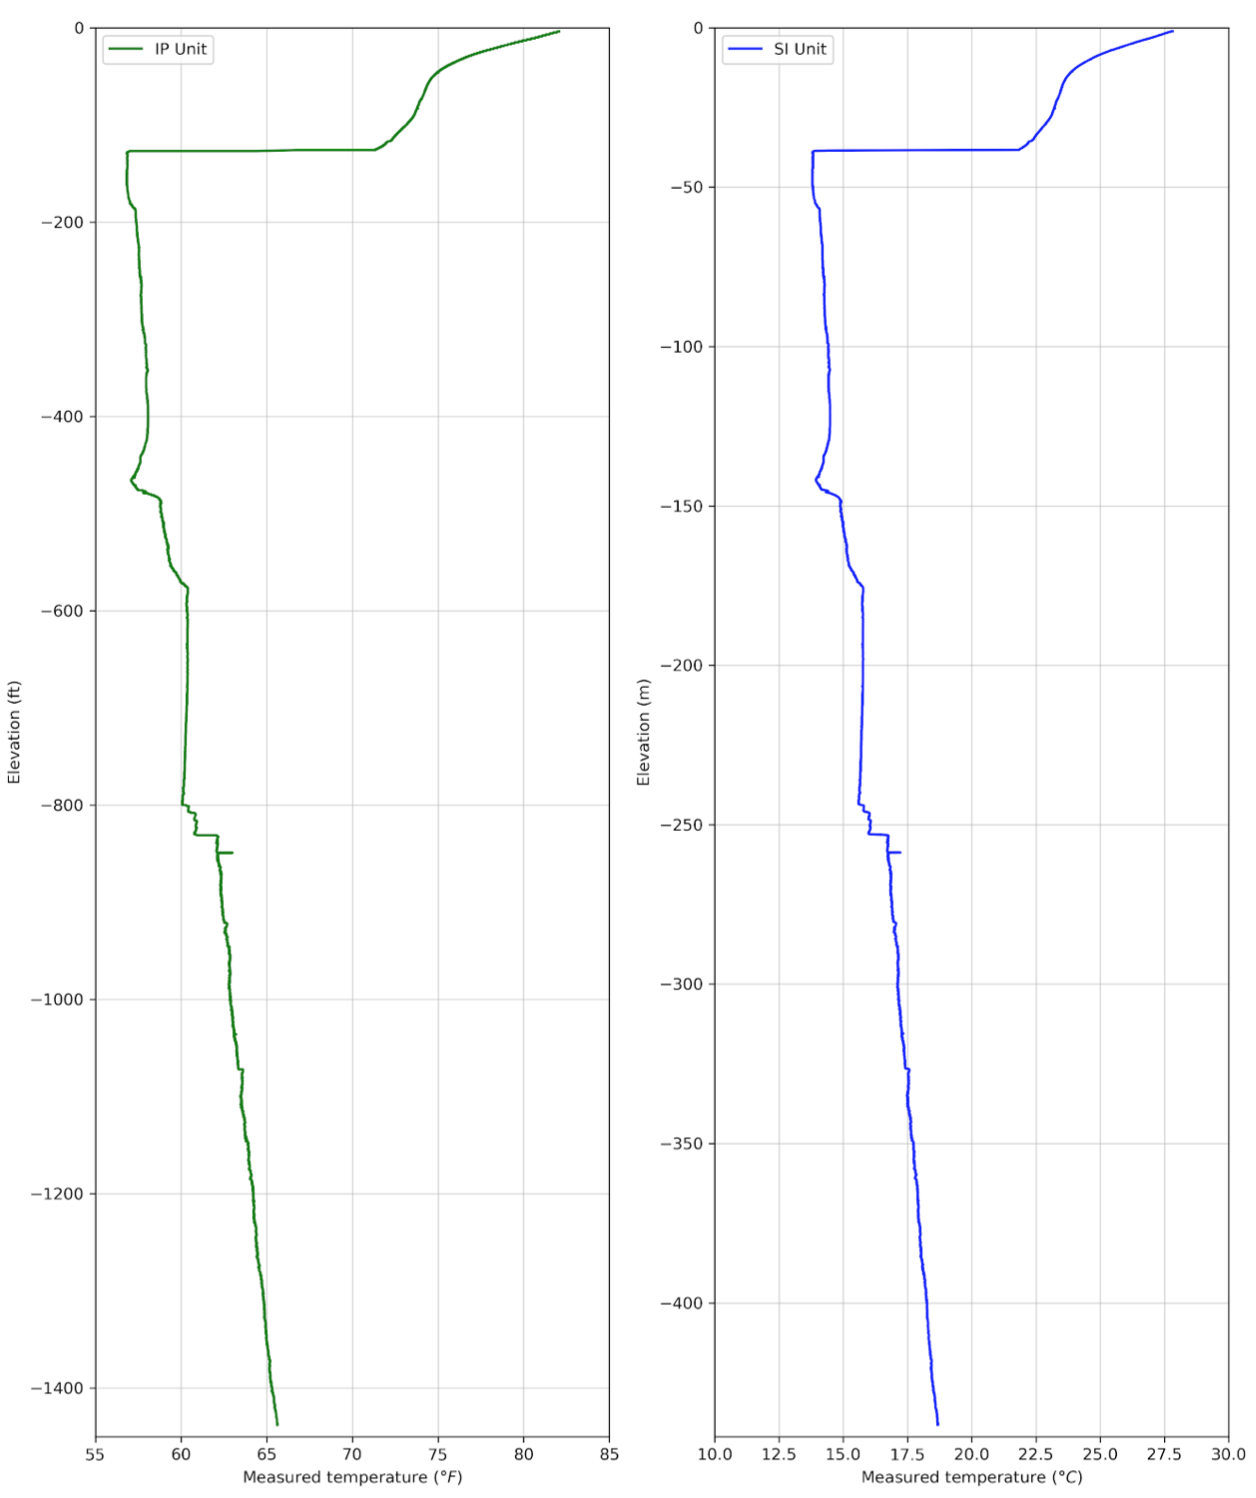
\includegraphics[height=0.5\textwidth]{data/groudref}
	\caption{Temperature measurement from fiber optic cable attached to the outside of CBHE at test site prior to the commencement of TRT.}	
	\end{figure}


\subsection{Parametric Study of other CBHE configuration}
	We're interested in improving the thermal performance of the borehole heat exchanger, particularly with respect to the designed and site-specific variables. 
	\subsubsection{Depth}
	    The largest motivation of this study was to investigate the influence of geothermal gradient on CBHE performance, and what that might mean when considering a CBHE design. The total length of the BHEs are conventionally determined through the guidelines set by ASHRAE Handbook \cite{american_society_of_heating_refrigerating_and_air-conditioning_engineers_2013_2013}, which was originally proposed by Ingersoll and Zobel \cite{ingersoll_heat_1955} and further adjusted by Kavanaugh \cite{kavanaugh_simulation_1985}. This method requires the thermal conductivity, diffusivity of the soil as well as the borehole thermal resistance per unit length, establishing a clear link between the depth of the CBHE with the resulting heat extraction rate variation along the borehole, but with no geothermal gradient assigned to the model, added depths only increases heat exchange area and not the reference ground temperature.
            
        Geothermal gradients are commonly known to be within 25 to 30 Kelvins per kilometer for shallower layers of ground \cite{holmberg_thermal_2016}. We therefore assume a geothermal gradient of  30 K per kilometer for this analysis where different depths could be used in designing a CBHE\cite{shrestha_assessment_2018}. This is to be expected to be representative of an average condition for deeper geothermal boreholes. For the undisturbed ground temperature profile, we used the measured data from Beier's research for the first 178 meters, and extrapolated the rest of the borehole length with the geothermal gradient we selected. We also held the rest of the borehole configuration constant, following the Beier study from 2013, changing only the depth of a borehole to achieve different vertical temperature profiles. To avoid the more transient first few hours, only the vertical temperature profiles at the 100th hour will be compared against one another. To better illustrate how this may affect the heat extraction rate, we will also be using a second set of legend to show the heat extracted averaged by length in $W/m$ from the borehole via Equation~\ref{eq:qout}. The results we will be showing in the vertical temperature profiles will be the 100th hour condition, and will remain so unless otherwise specified in the legend and caption. 
            
                \begin{equation}
                    q_{out}=c_w\dot m \frac{T_{out}-T_{in}}{L}\label{eq:qout}
                \end{equation}
                     
        We picked five borehole lengths at 50 m, 150 m, towards the deeper ones at 500 m , 1000 m, 1500m and 2000 m as an extreme to examine the temperature distribution vertically with the original horizontal borehole configuration as shown in Beier's research \cite{beier2013}. We examined both the comparison plot with the actual and dimensionless depth as the y-axis to determine the more legible option. It is expected that the base case will have much of the thermal energy available at the bottom of borehole taken away due to a smaller shunt resistance. Increasing the shunt resistance could theoretically improve the thermal performance of the boreholes.
            
        Intuitively, a good design intervention to increase the thermal performance of CBHE is to insulate the inner pipe. To demonstrate how insulation alone could change the thermal performance of a CBHE, we also examined an ideal case where we assume the insulation material that we calculate $R_{ins}$ from is vacuum. We do so by assuming CBHE has vacuumed space as the insulating material, resulting in a thermal conductivity of $k_{pp}=0.007 W/(m\cdot K)$ across the shunt and thus, giving a best case scenario of the temperature profile and heat extraction rate. It is important to point out the vacuum case is merely an ideal and hypothetical scenario instead of a realistic one. Even with a somehow vacuumed insulating inner paper, it is highly unlikely that the vacuum can be maintained during prolonged CBHE operation, i.e. can be used for actual implementation for a CBHE. The vacuum scenario is, at its best, an ideal condition that illustrates the best operating scenario with a super-insulated central pipe, or how helpful insulation could be in when designing CBHE operating with a larger bottom of borehole temperature. It should be noted that this is highly unlikely to be achievable by actual CBHEs, since not only will there be additional engineering challenges in addressing the decreased average density of the shunt, there will also need to be separate analysis on how to properly insulate a CBHE to maintain its long-term insulated performance, all assuming that the added cost of insulating the inner pipe can be justified. 

        		We obtained the vertical temperature distribution as shown in Figure ~\ref{fig:Depths}.        \begin{figure}[h!]
            \centering
            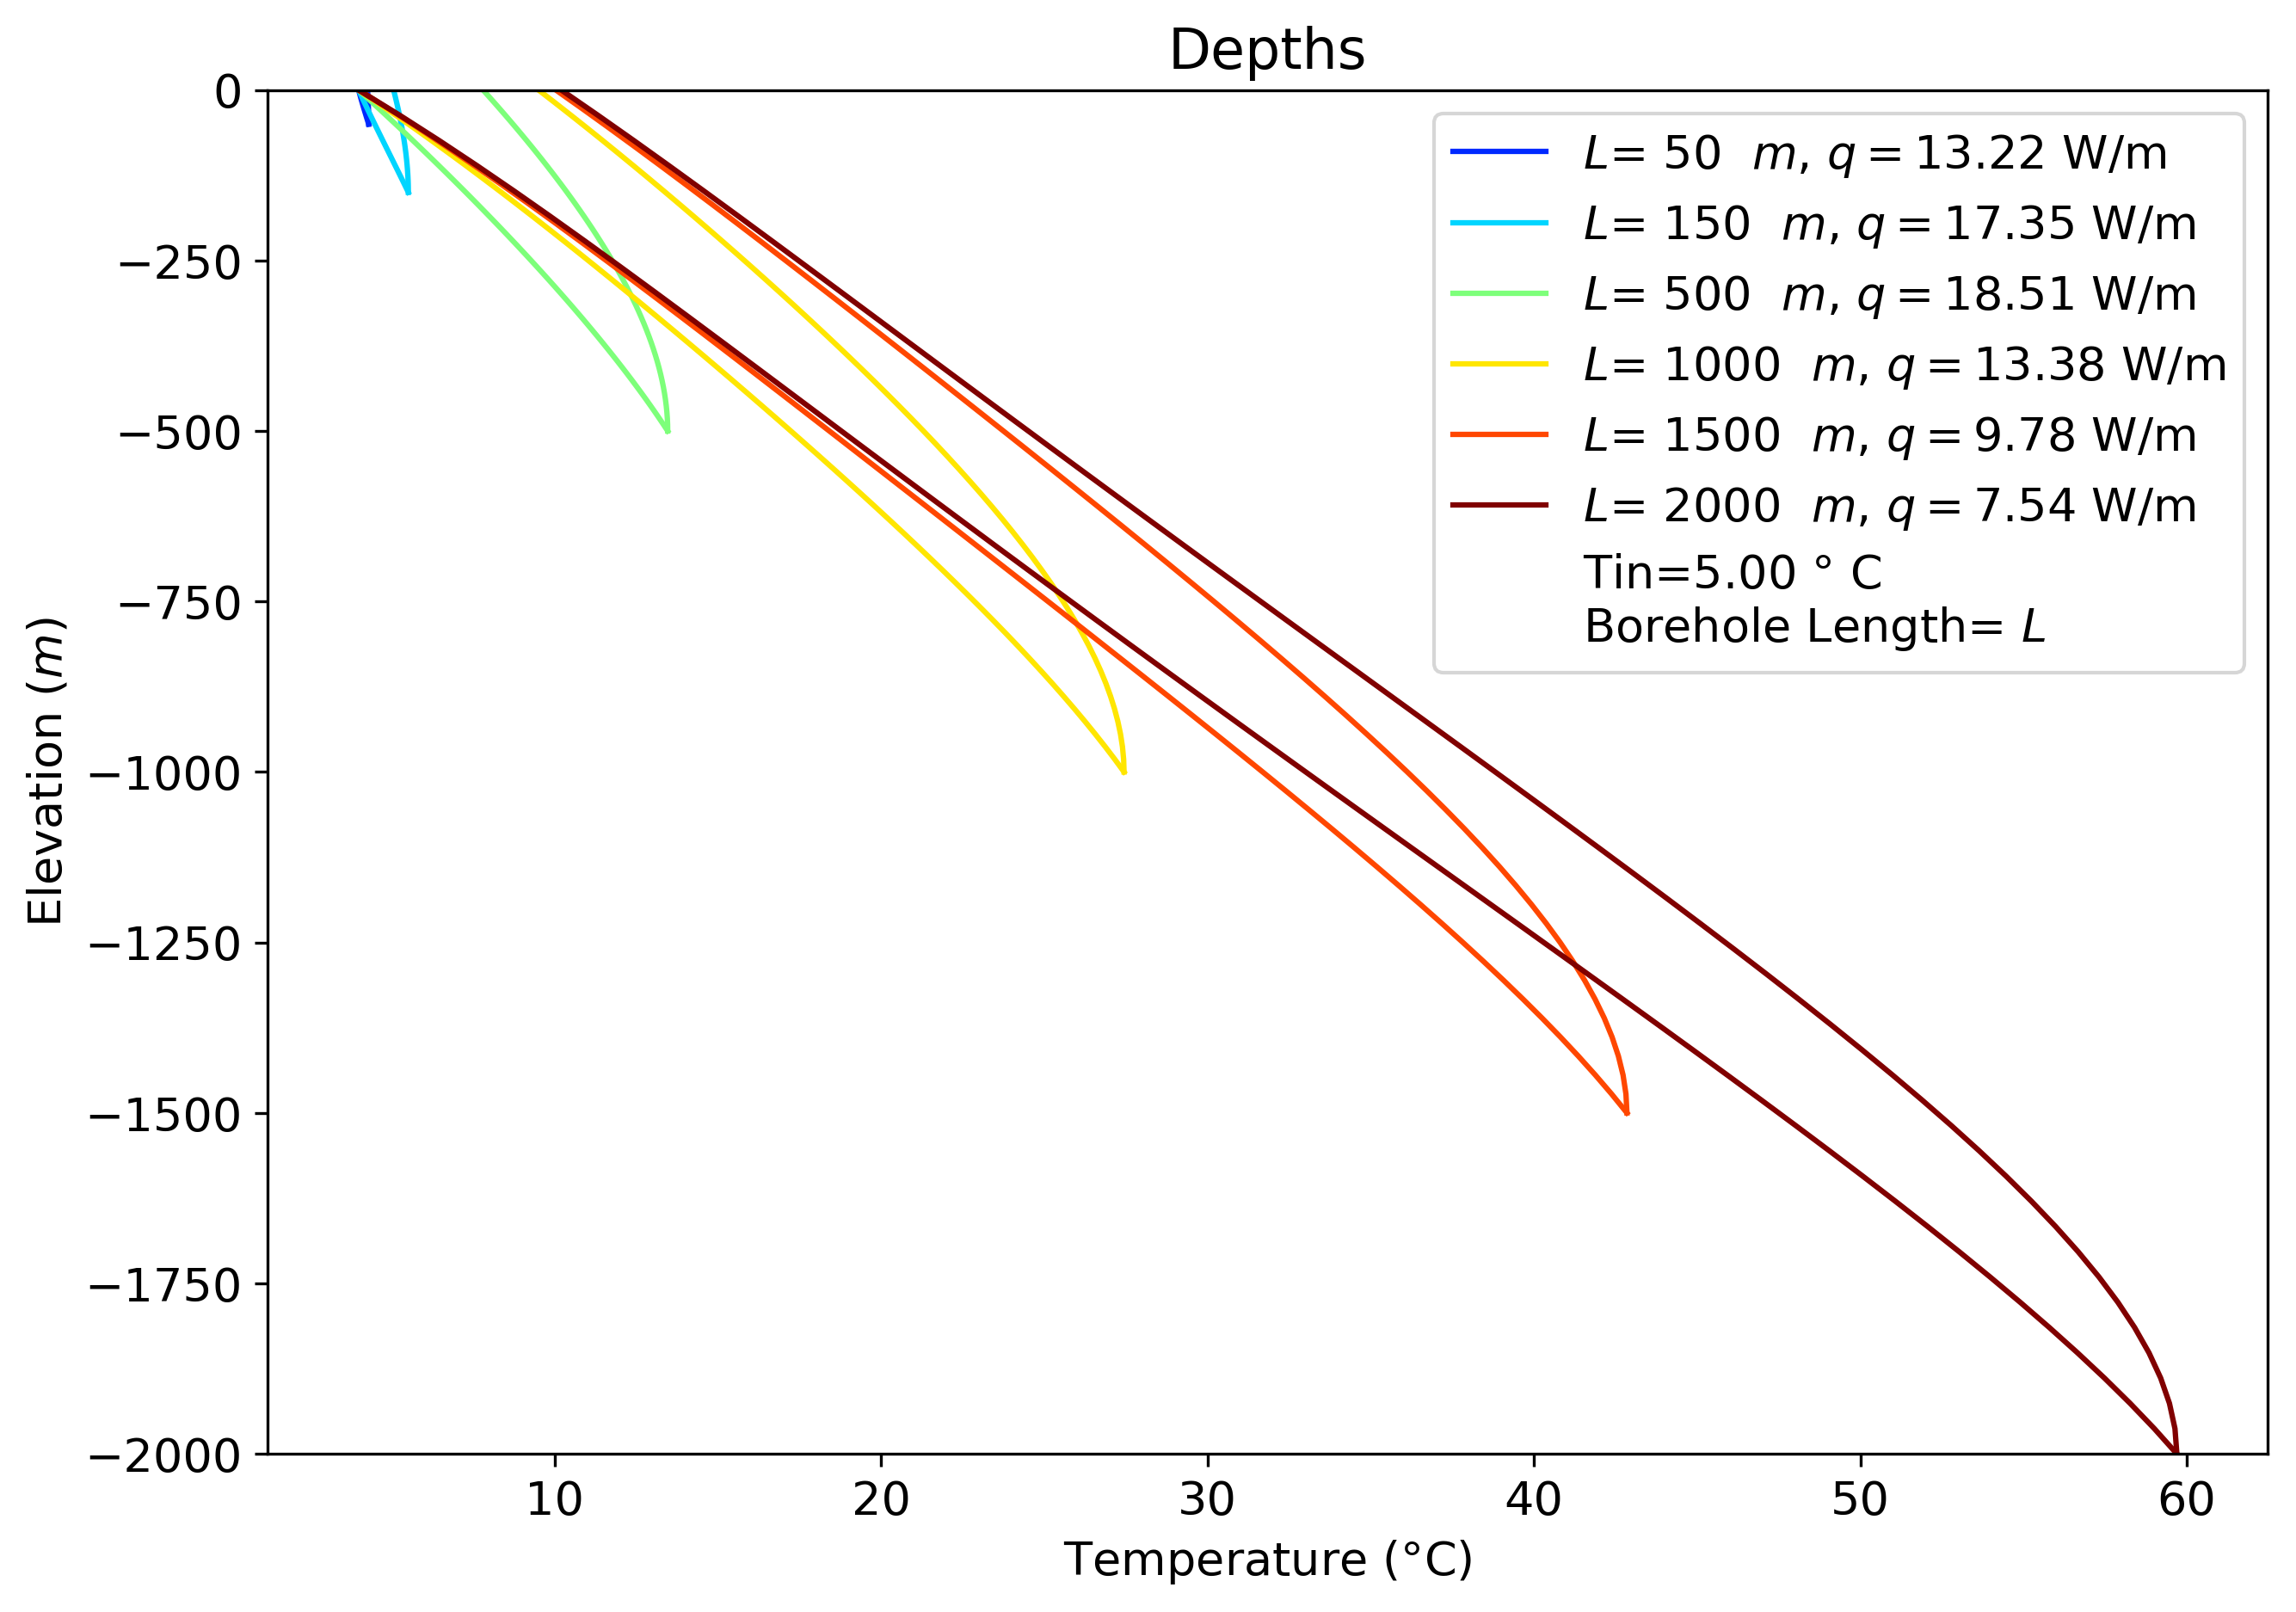
\includegraphics[width=0.65\textwidth]{depths_5_TrueDepth.png}
            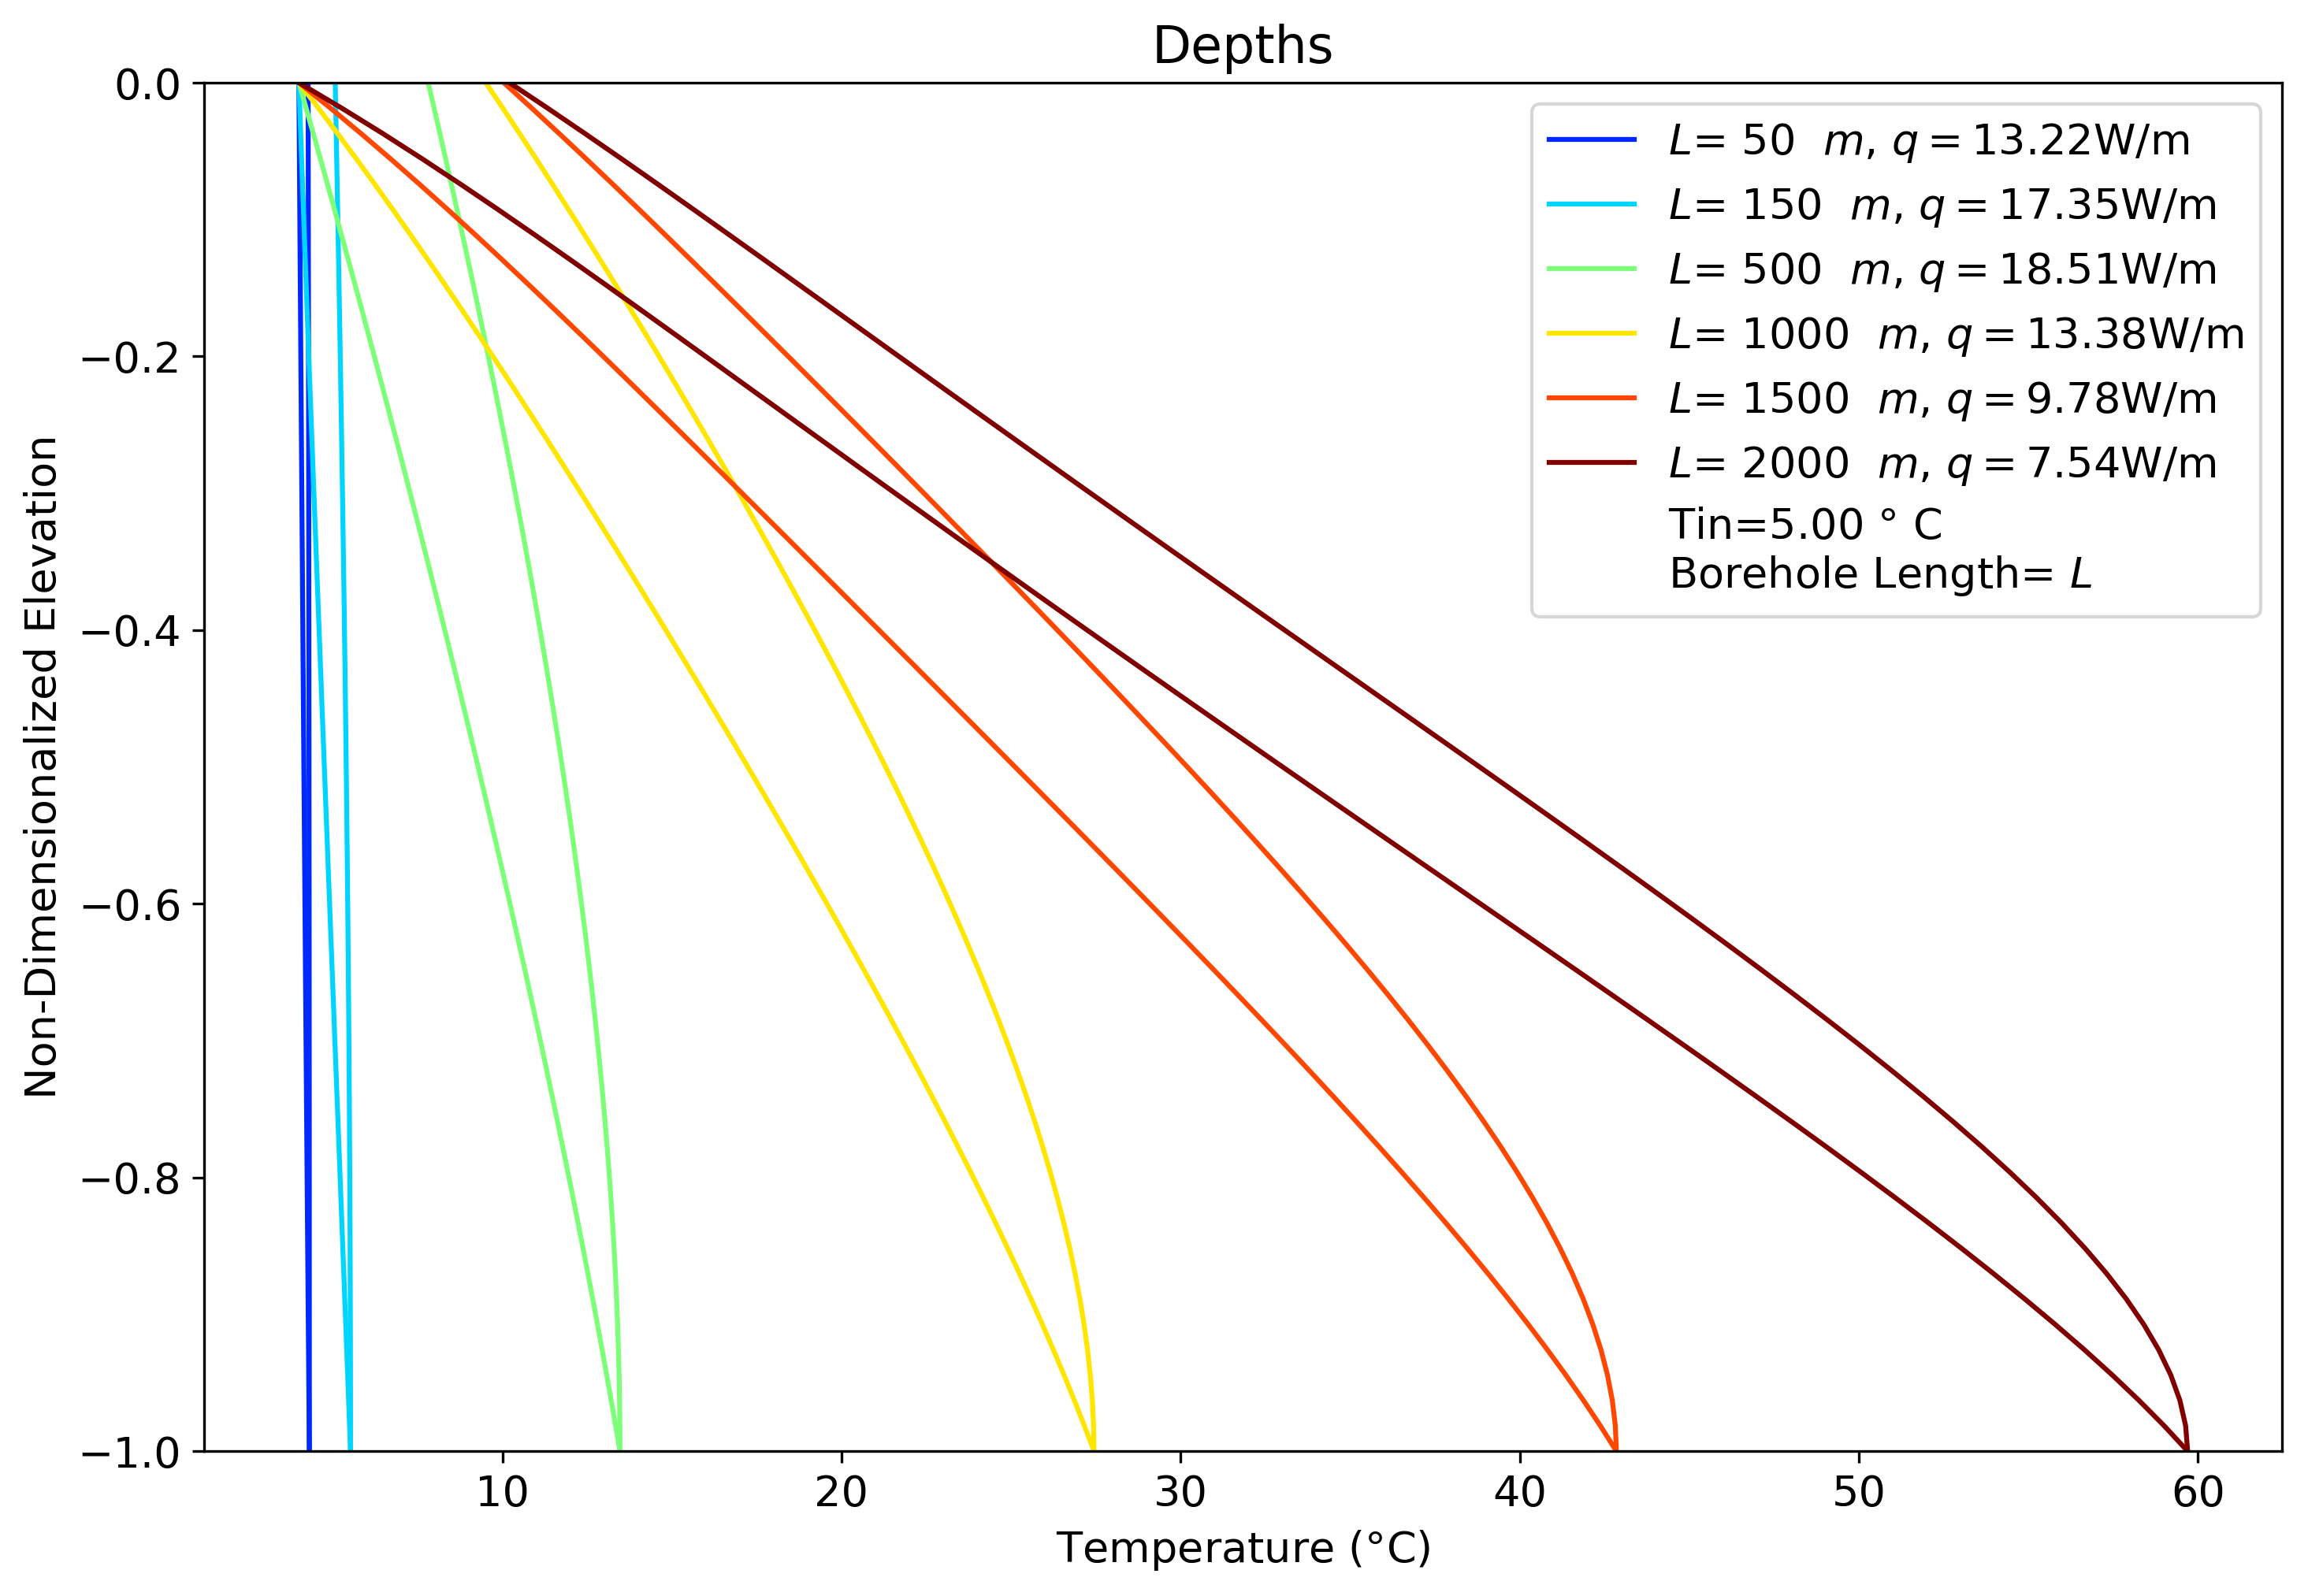
\includegraphics[width=0.65\textwidth]{depths_5.png}
            \caption{Actual vertical temperature distribution of CBHE with length of 50, 150, 500, 1000, 1500, 2000 m with actual depths (left) and dimensionless depths (right).}
            \label{fig:Depths}
        \end{figure}
		We obtained the vertical temperature distribution as shown in Figure ~\ref{fig:Depths}. As expected, the presence of geothermal gradient leads to increased heat extraction rate for deeper boreholes. The heat extraction rate, however, does not increase proportionally with the depth increase, as the amount of heat extracted only increased by approximately 12.6\% when the assumed CBHE length increases from 1000 m to 2000 m. The amount of extra investment to both drill the borehole and the additional cost of in casing to avoid borehole collapsing could also be significant. Between the six depths tested, it appears that a preferred length of CBHE could be 1000m, since the heat extraction rate exhibit the most significant jump for the first kilometre only for a CBHE whose far-field temperature distribution is driven by geothermal gradient at 3 Kelvin every 100 meters only. The length of a CBHE is therefore set to be at 1000 m for the remainder of this study. An interesting trend for temperature evolution along the discharge pathway is that the inlet and outlet appeared coupled, while the heat exchange between the inlet and outlet pathways works against the purpose of heat extraction.
        
		To best avoid the heat transfer between the two pathways, i.e. using an artificial scenario where the inner pipe is vacuumed to achieve a thermal conductivity of vacuum where $k_{pp}$ = 0.007 $W/(m\cdot K)$, the temperature distribution and heat extraction rate shown in Figure~\ref{fig:Depths} becomes Figure~\ref{fig:kpp007}. The heat extraction rate drastically increases, despite the thermal conductivity being hypothetical and potentially challenging to reach for a real CBHE as the inner piping can easily float out from the CBHE well driven by its buoyancy. Most materials become succumb to the hurdle where the smaller the thermal conductivity, the lower the material density.  Alternatively, an inner pipe that is double-layered and vacuumed in between could also help achieve the best insulation, yet not only will the manufacturing be challenging, there's also an explicit economic constraint for a deeper CBHE. It is therefore essential to seek alternative methods to achieve maximised heat extraction rate, or more specifically, whether it might be possible to achieve comparable if not better heat extraction rate by making incremental changes to a CBHE design.
        \begin{figure}[h!]
            \centering
            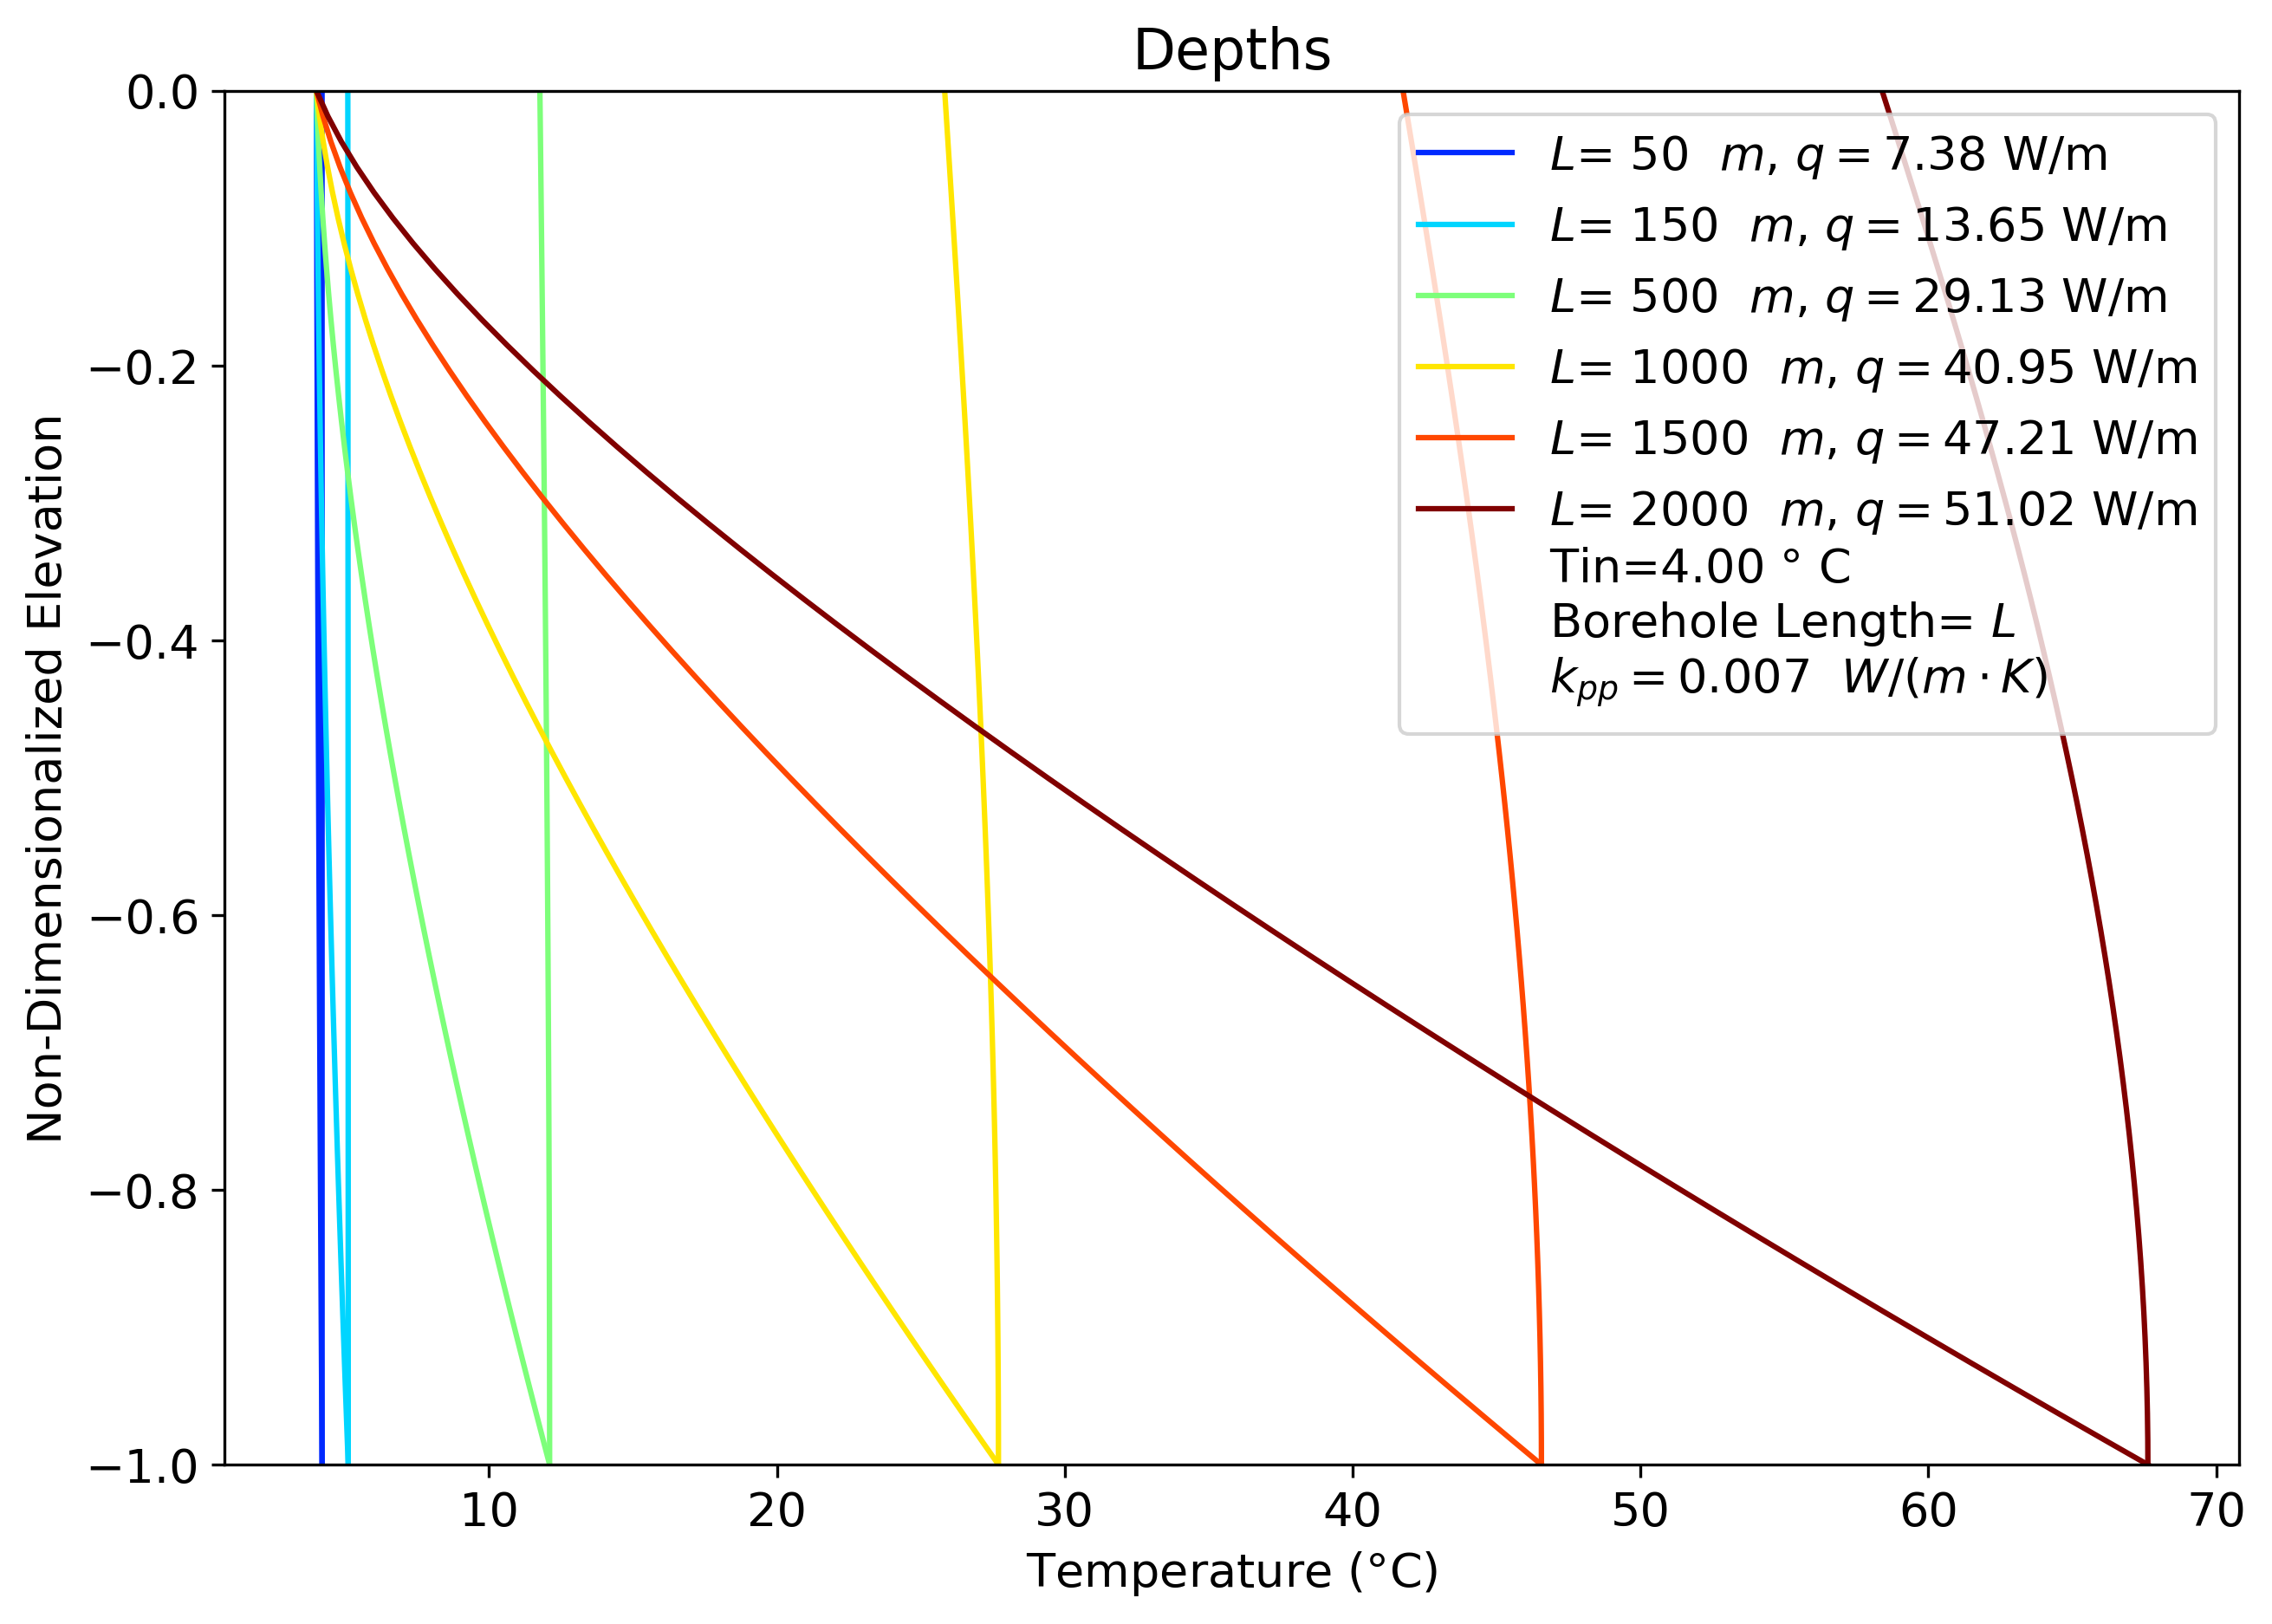
\includegraphics[width=.65\textwidth]{depths_5_kpp007.png}
            \caption{Vertical temperature distribution of CBHE with length of 50, 150, 500, 1000, 1500, 2000 m with non-dimensionalized depth with added assumed insulation of $k_s=0.007 W/(m\cdot K)$.}
            \label{fig:kpp007}
        \end{figure}
    \subsubsection{Insulation}
    	As was mentioned above, adding insulation to the inner wall of a CBHE appears to be an ideal solution to ensure maximized heat extraction at a larger depth. To reduce the material and construction cost of a CBHE, a natural question to ask is whether decreasing the thermal conductivity of the inner pipe and increasing its thickness could lead to improved overall heat and temperature extraction. This is analyzed by assuming the borehole length is 1000 meters, which appears to be a relatively good depth to observe the influence of geothermal gradient according to our previous results obtained on the depths analysis.
        
		For thermal conductivities of the inner pipe, the commercially available PP piping has a $k_{pp}$ ranging from 0.19 to 0.5 $W/(m \cdot K)$ for PP piping and results in apparent changes of vertical temperature profiles and heat extraction rate as is shown in Figure 4. The smallest thermal conductivity of the material used was 0.19 $W/(m \cdot K)$, resulting in a larger shunt resistance $R_{12}$ and hence a better heat extraction rate. With the thermal conductivity increasing to 0.5 $W/(m \cdot K)$, the heat exchange between the central and annular flow gradually increases, causing a gradual increase of the short-circuiting of the CBHE - the flow travelling upward loses more heat to the inner pipe as it travels to near ground-surface. 
        
        \begin{figure}[h!]
            \centering
            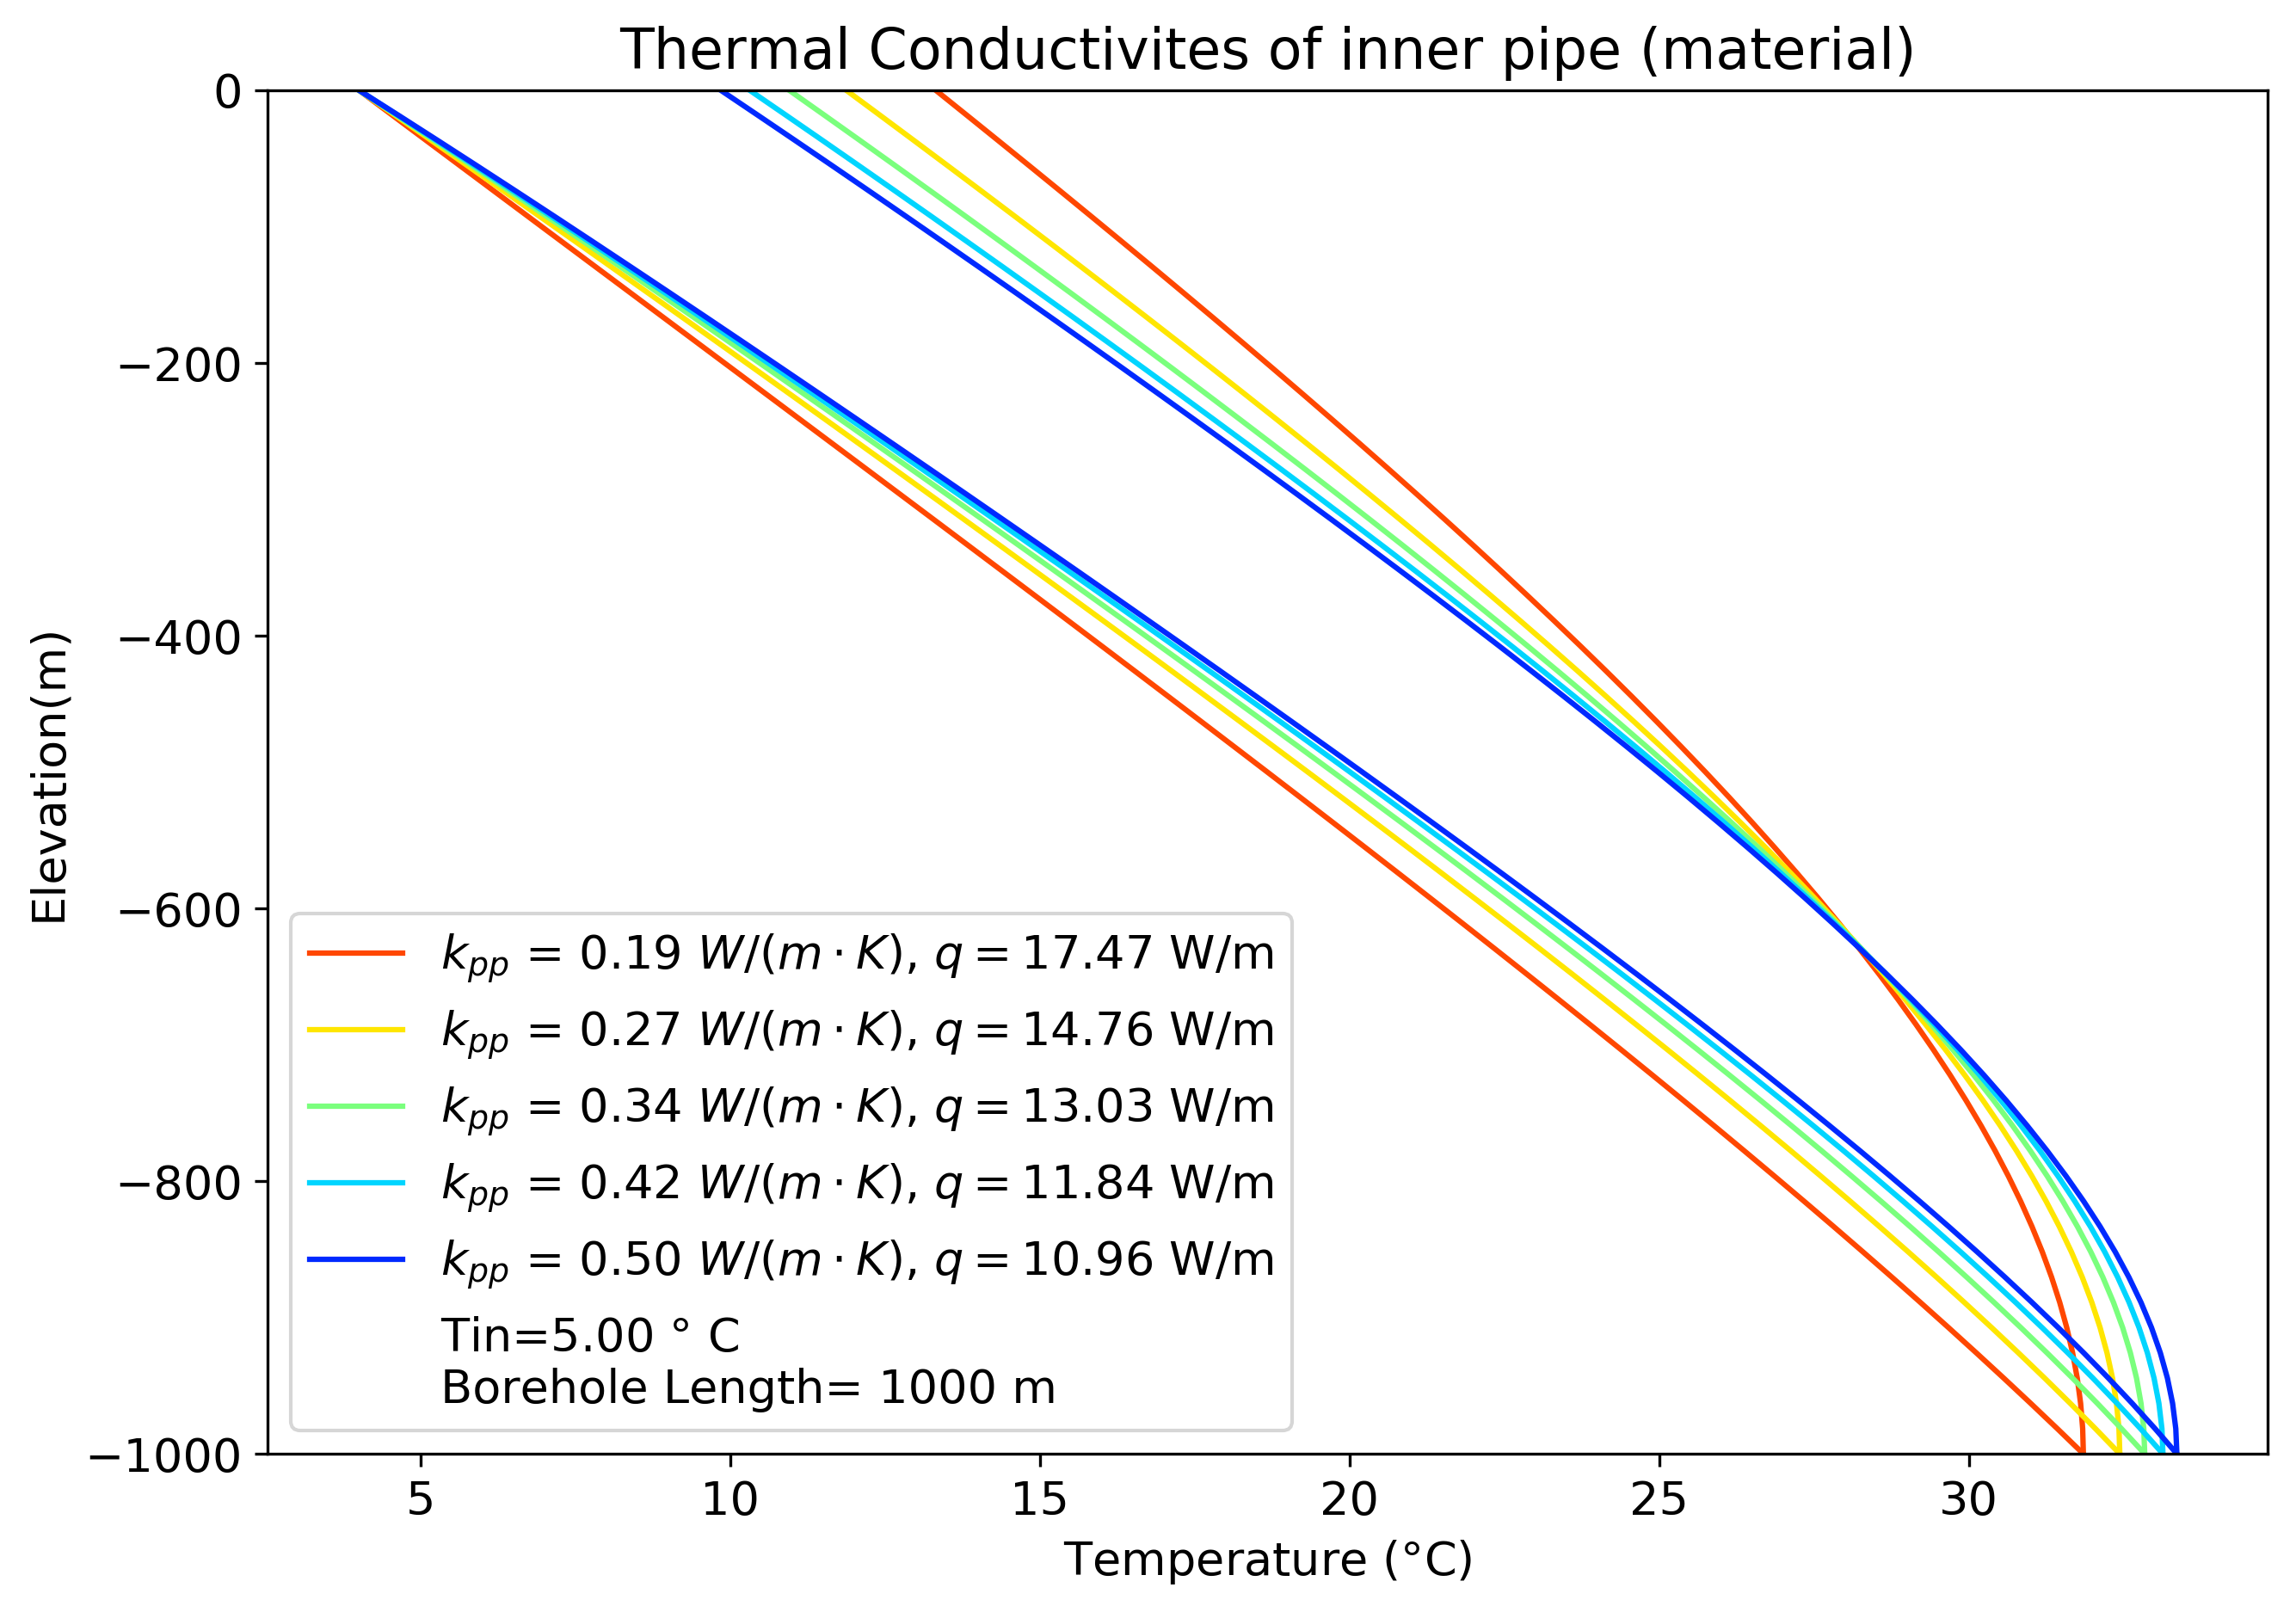
\includegraphics[width=0.65\textwidth]{kpp_500_MIN.png}
            \caption{Vertical temperature distribution profiles resulting from variation of thermal conductivity of the outer pipe at the 100th hour of simulation.}
            \label{fig:kpp}
        \end{figure}
        
		We then further modified the CBHE configuration by varying the thickness of the inner pipe wall, such that the shunt thermal resistance also increases such that the heat exchange between the inlet and outlet can be decreased further. Varying the thickness of the inner pipe and holding the inner pipe diameter constant, the actual cross-section area of the inner pipe (AD1) reduces as the area ratio $r_{12}$ increasing, and we were able to obtain Figure~\ref{fig:thickness}. Increasing the thickness of the inner pipe from 3 mm to 19 mm changes the vertical temperature distribution inside the CBHE at the 100th hour. Altering the thickness of the inner pipe appears to have effectively increased the heat extraction rate and minimised the heat transfer through the shunt, leading to a much-improved temperature decrease along the central pipe for the flow upward.
         
        \begin{figure}[h!]
            \centering
            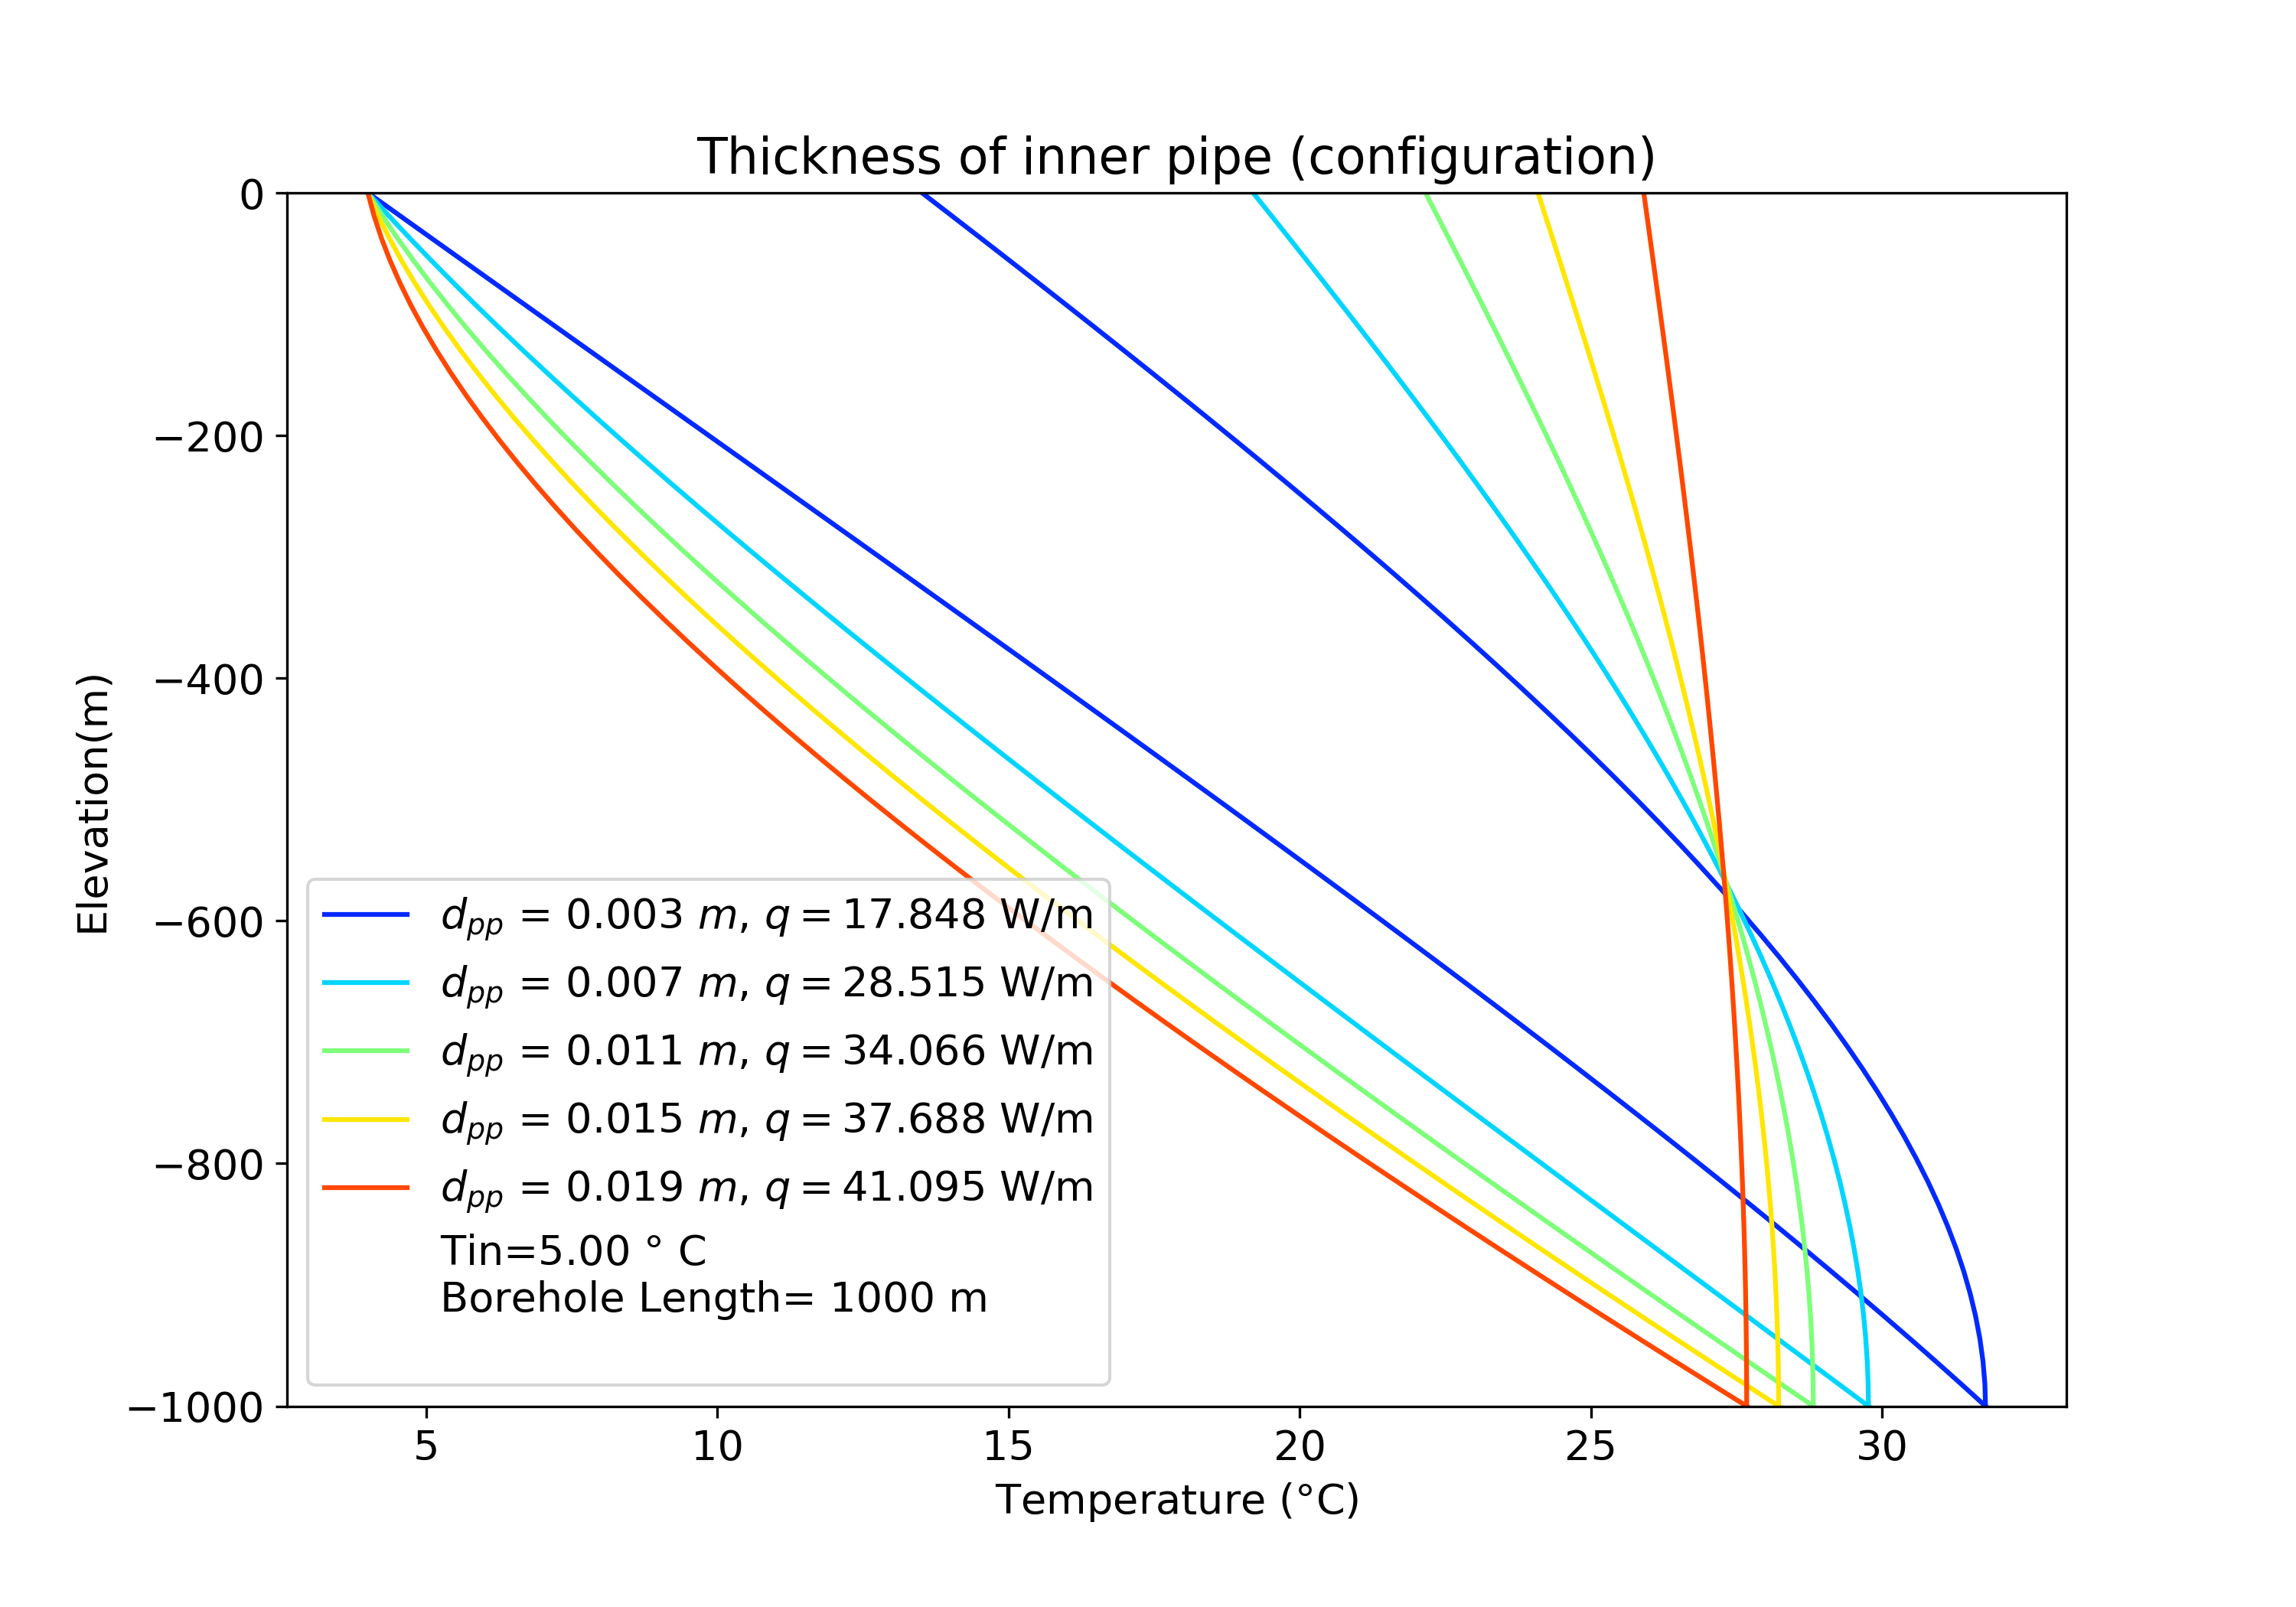
\includegraphics[width=0.65\textwidth]{dpp_500_MIN.png}
            \caption{Vertical temperature distribution profiles resulting from variation of inner pipe thickness of the outer pipe at the 100th hour of simulation.}
            \label{fig:thickness}
        \end{figure}
        
		The resulting heat extraction rate with the most substantial thickness exceeds the heat extraction rate obtained in the fictional thermal conductivity assumed in Figure~\ref{fig:kpp007} for the 1000 m deep CBHE at 41.095 W/m at the 100th hour of the simulation. A natural question then arises on whether it would also make sense for the outer pipe when its thermal resistance is minimised, could have improved the thermal performance of CBHE at a similar order of magnitude. To do so, we first examine the results of varying the thermal conductivity of the outer pipe in Figure ~\ref{fig:kep}. It does not appear to have as significant an effect on the resulting temperature distribution at the 100th hour as shown in Figure ~\ref{fig:kep}.
        
        \begin{figure}[h!]
            \centering
            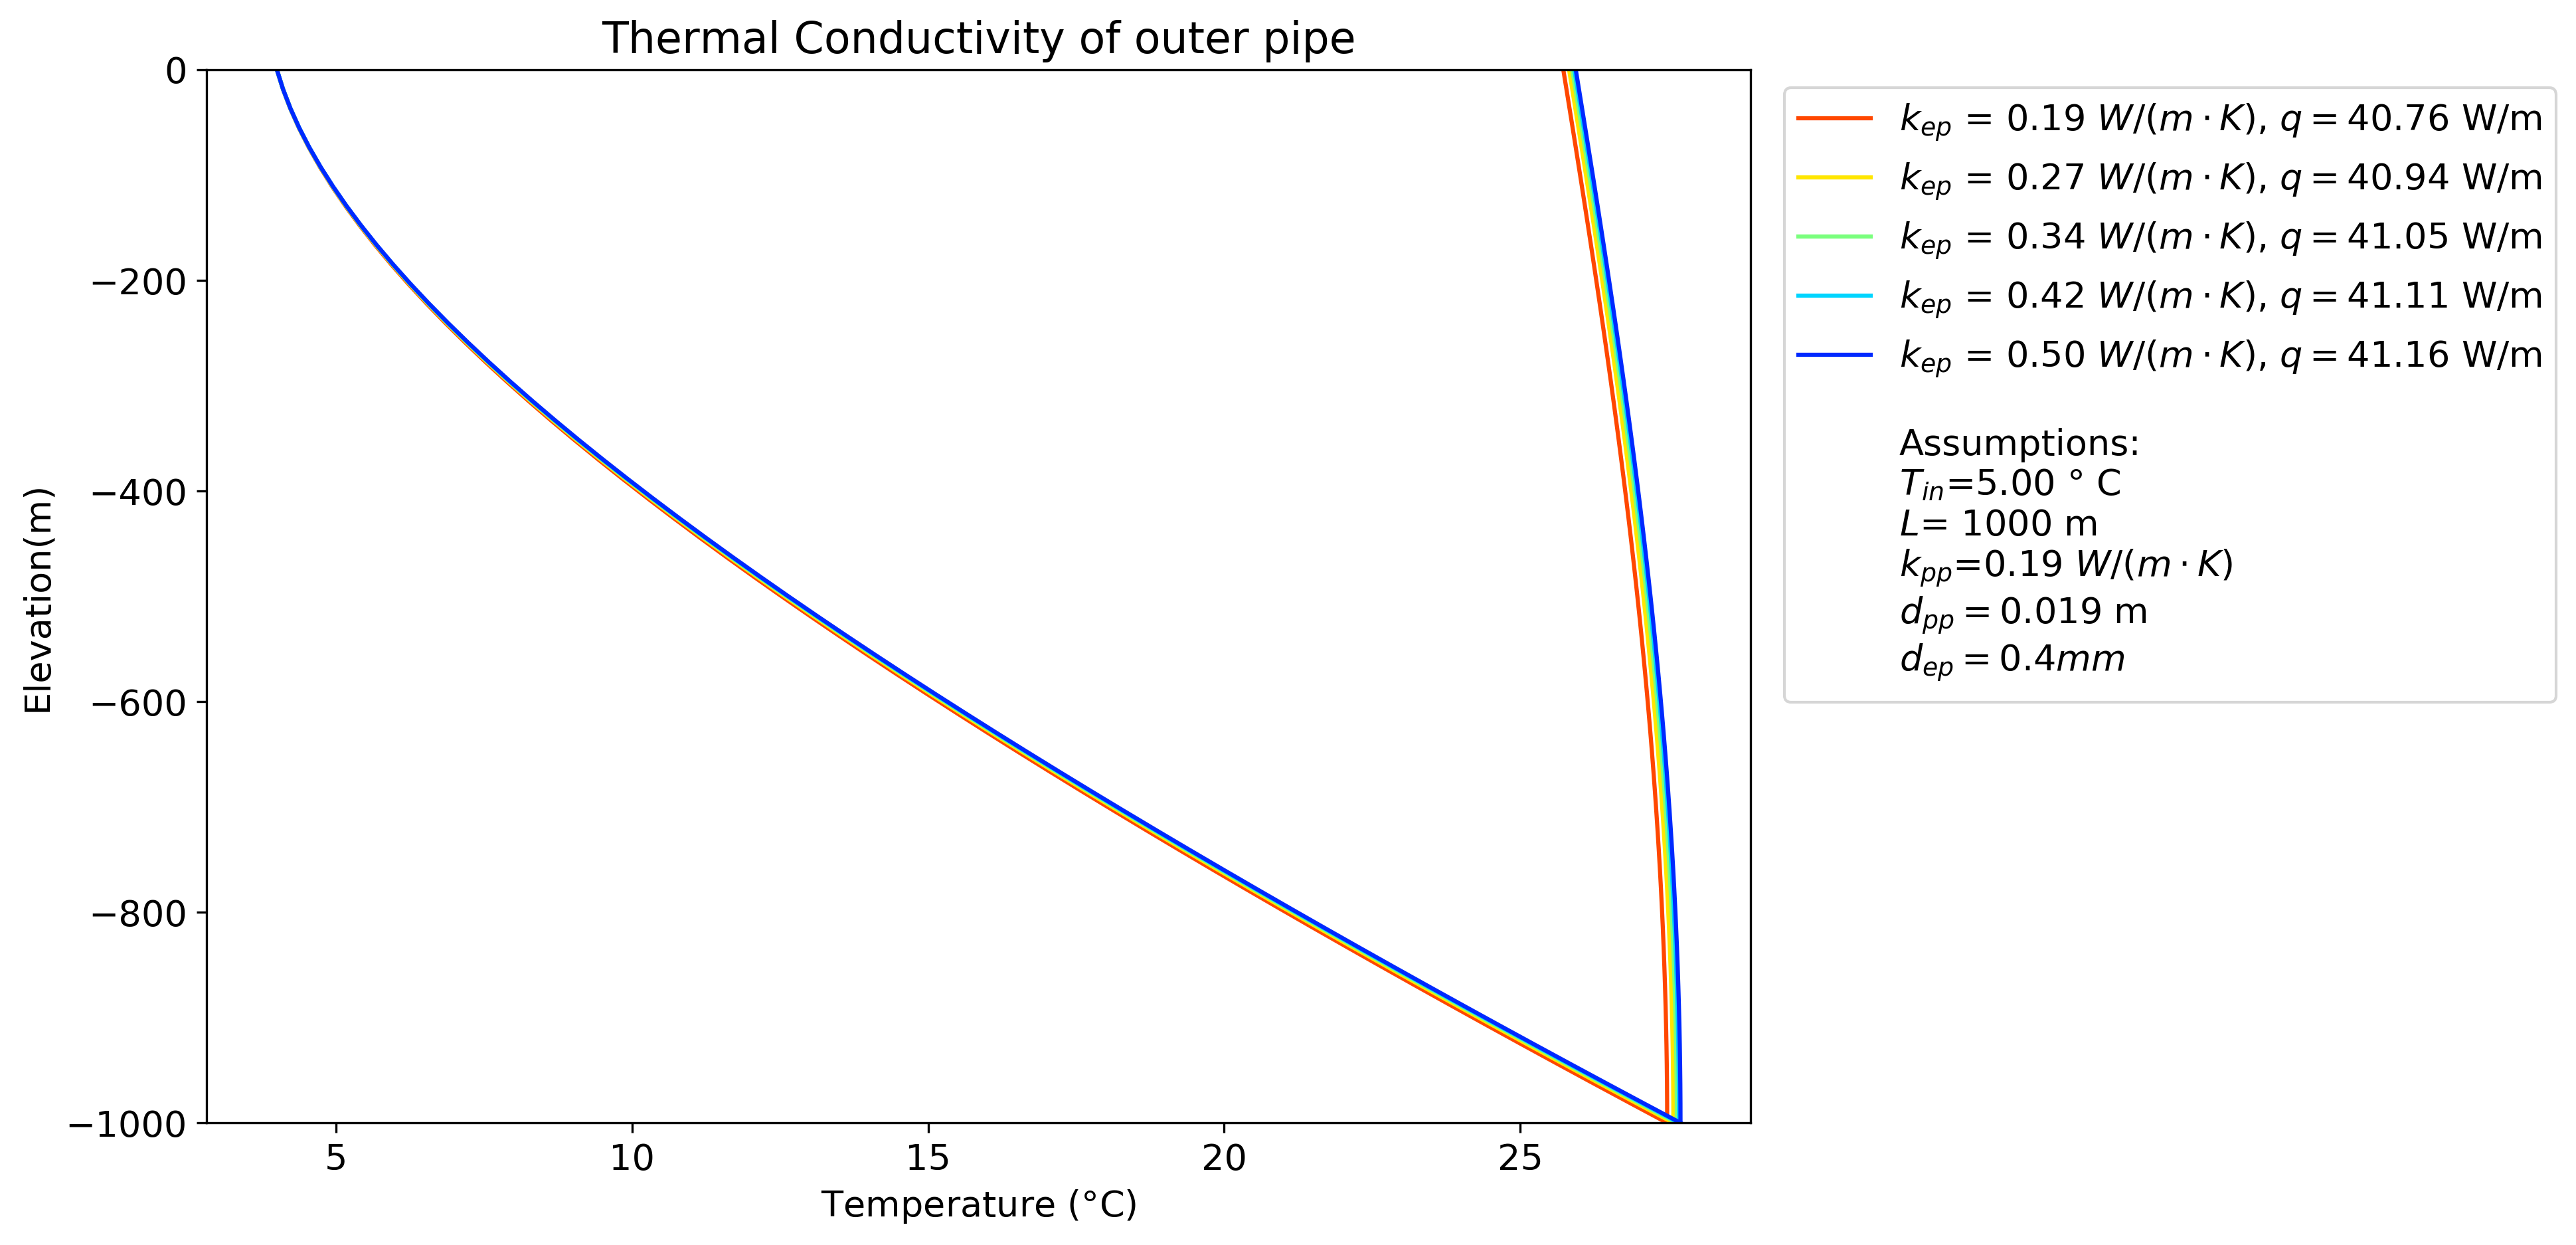
\includegraphics[width=0.75\textwidth]{kep_1000_MIN.png}
            \caption{Vertical temperature distribution profiles resulting from variation of thermal conductivity of the outer pipe at the 100th hour of simulation.}
            \label{fig:kep}
        \end{figure}
        
		To better examine the result of varying the outer wall thickness and the resulting temperature profiles, we analysed different $k_{ep}$ from 0.5 $W/(m \cdot K)$, as well as $k_{pp}$ at 0.19 $W/(m \cdot K)$, which led to results shown in Figure~\ref{fig:thickkep}. The thicker the outer pipe, the slower the heat extraction along the annulus, and the smaller amount of heat extraction rate at the inlet/outlet of the borehole, as can be observed from Figure~\ref{fig:thickkep}. It is vital, therefore, to keep the thermal conductivity for the outer pipe as large as possible, while maintaining the thickness of the outer tube as small as possible. Hence the thermal conductivities of the inner and outer pipe becomes $k_{pp}$ = 0.19$W/(m \cdot K)$, $k_{ep}$ = 0.50$W/(m \cdot K)$, while the thickness of the inner and outer pipe becomes $d_{pp}$ = 0.019m, $d_{ep}$ = 0.0004m. We selected $d_{ep}$ following the Beier publication as an identified thinnest outer pipe CBHE.
        \begin{figure}[h!]
            \centering
            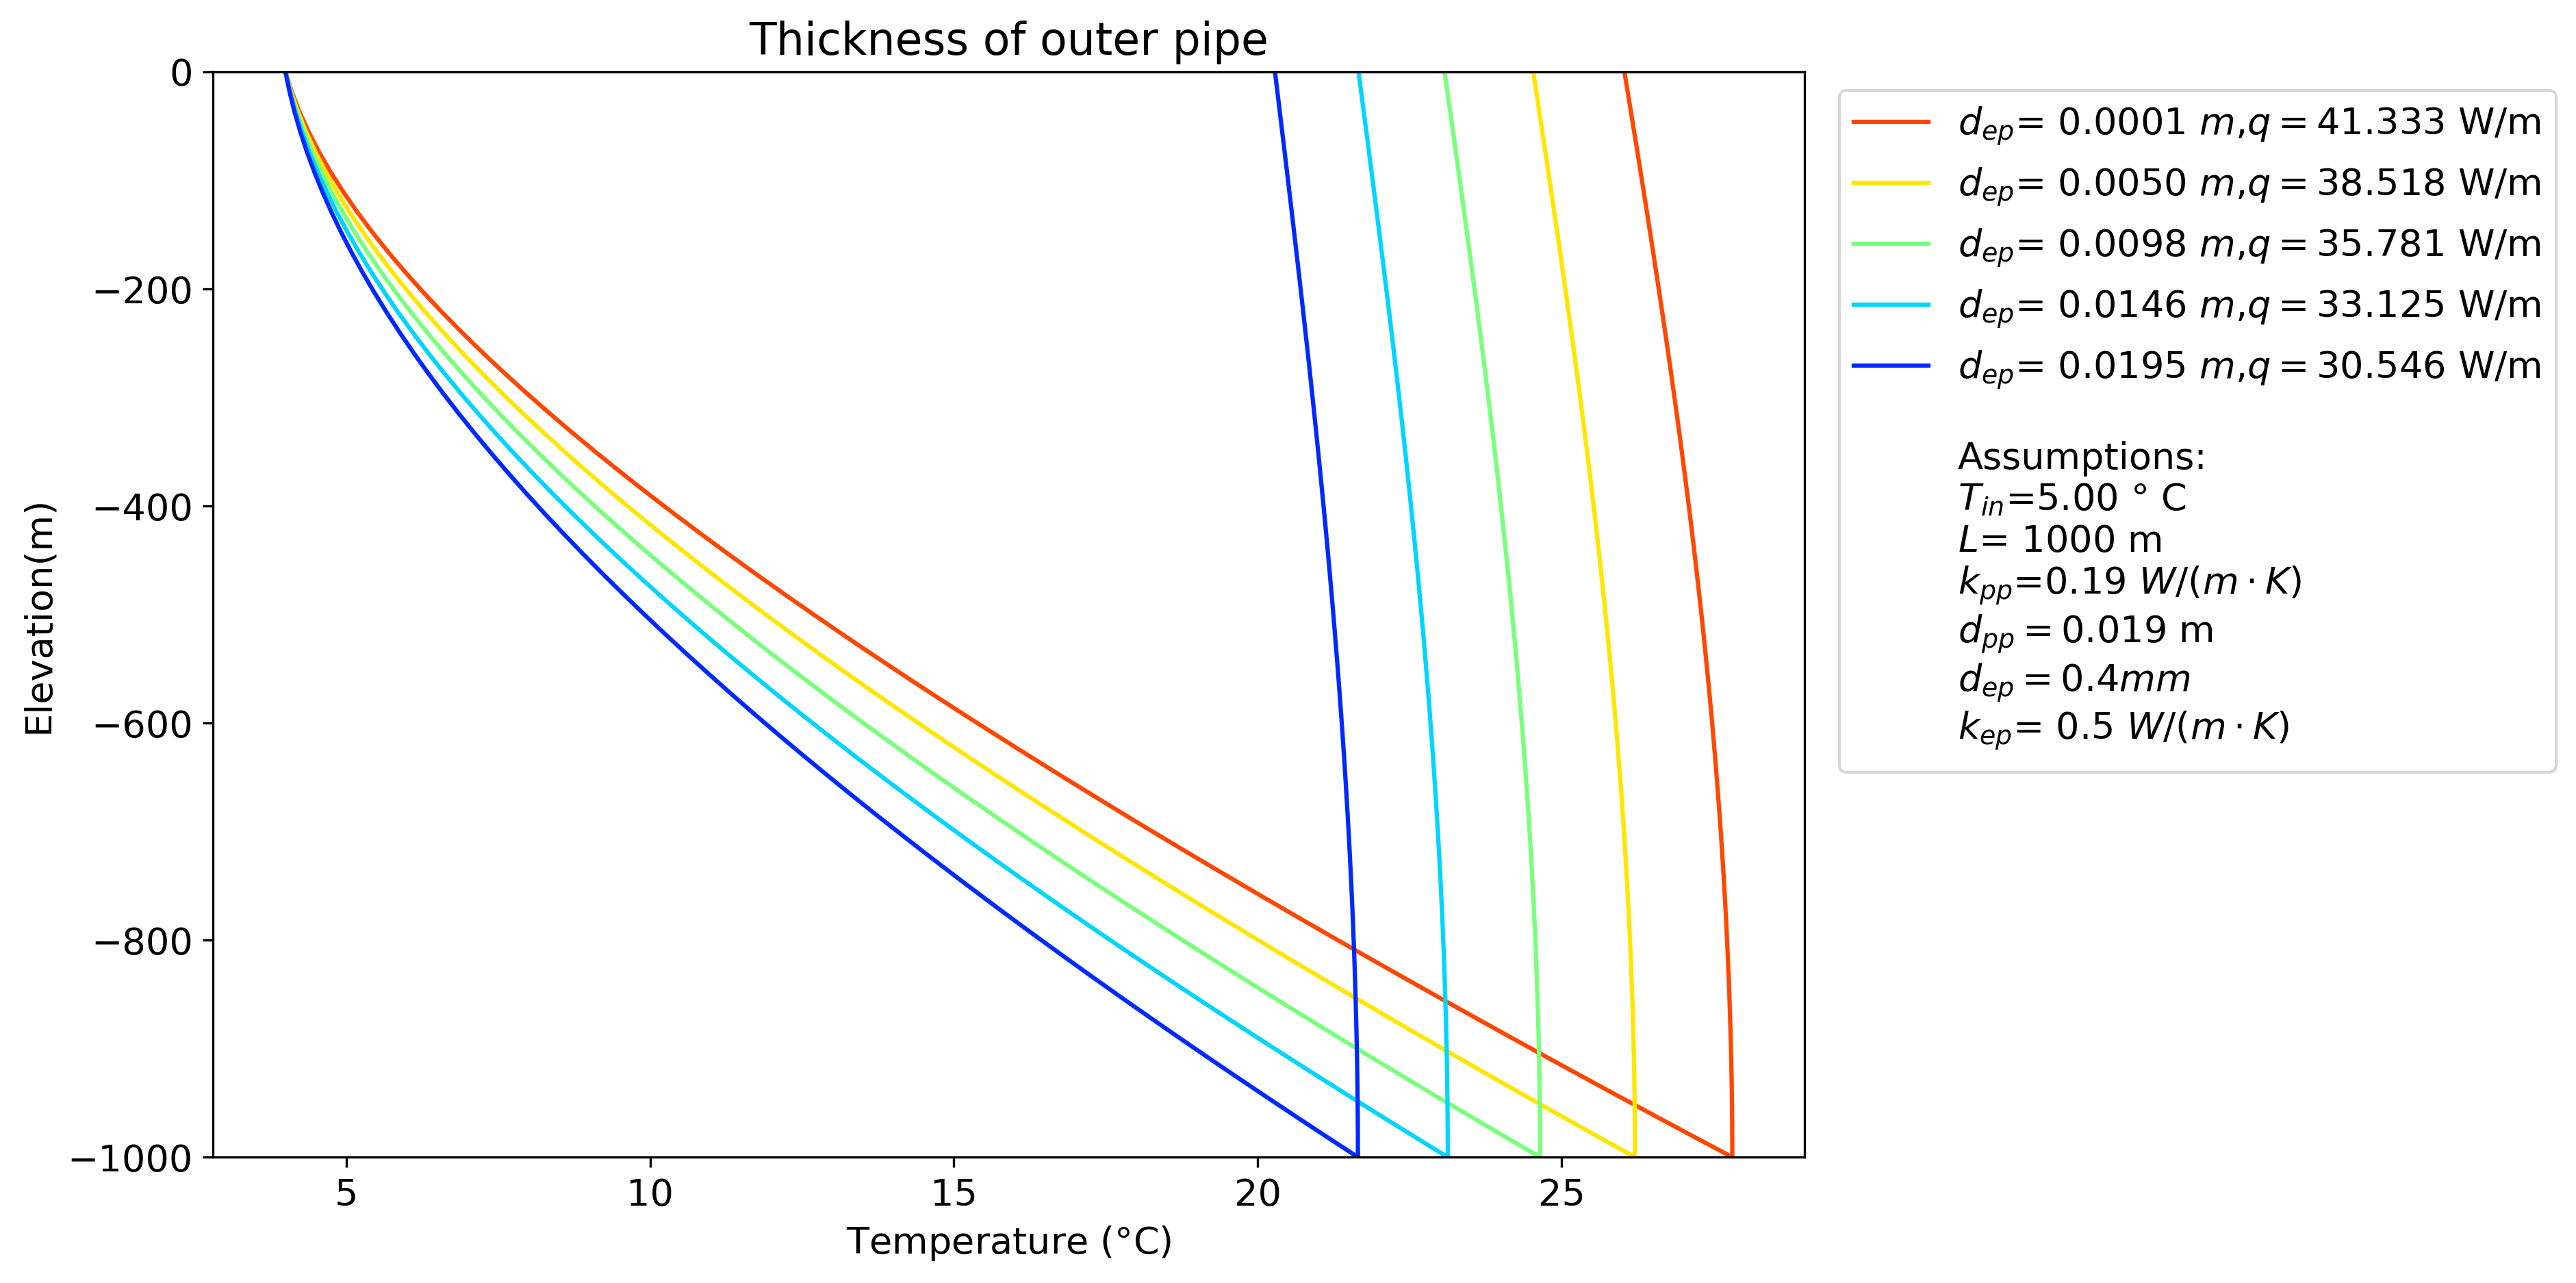
\includegraphics[width=0.75\textwidth]{dep_1000_MIN.png}
            \caption{Vertical temperature distribution profiles resulting from variation of thickness of the outer pipe at the 100th hour of simulation.}
            \label{fig:thickkep}
        \end{figure}
		
		Additionally, these results could suggest improved performance inside standing column wells when they are deep and come into contact with the warmer ground due to the geothermal gradient. Without having a thermally conductive grout, a standing column well may have a considerably better performance when the wells are deeper with larger surfaces for heat exchange. The primary challenge for modelling standing column wells might be the added friction from not having smoother PVC pipes as flow channels, resulting in difficulties both in terms of modelling as well as operational cost increase.
    \subsubsection{Flow rates}
        Varying the flow rate inside the CBHE will also naturally lead to variations of the vertical temperature profiles. Hence we compared the configuration selected so far with a specific set of flow rates, ranging from laminar flow to turbulent flow, from 0.0001 to 0.005 $m^3/s$, as shown in Figure ~\ref{fig:frs}. As the flow rate increases, the heat extraction rate also increases. Observing the vertical temperature distribution variation over time under different flow rates, as shown in Figure ~\ref{fig:FR3_dev}, the temperature profiles coloured concerning how far along the simulation went, with the initial conditions marked as blue, and the last states marked out as dark red/brown.
        
        \begin{figure}[h!]
            \centering
            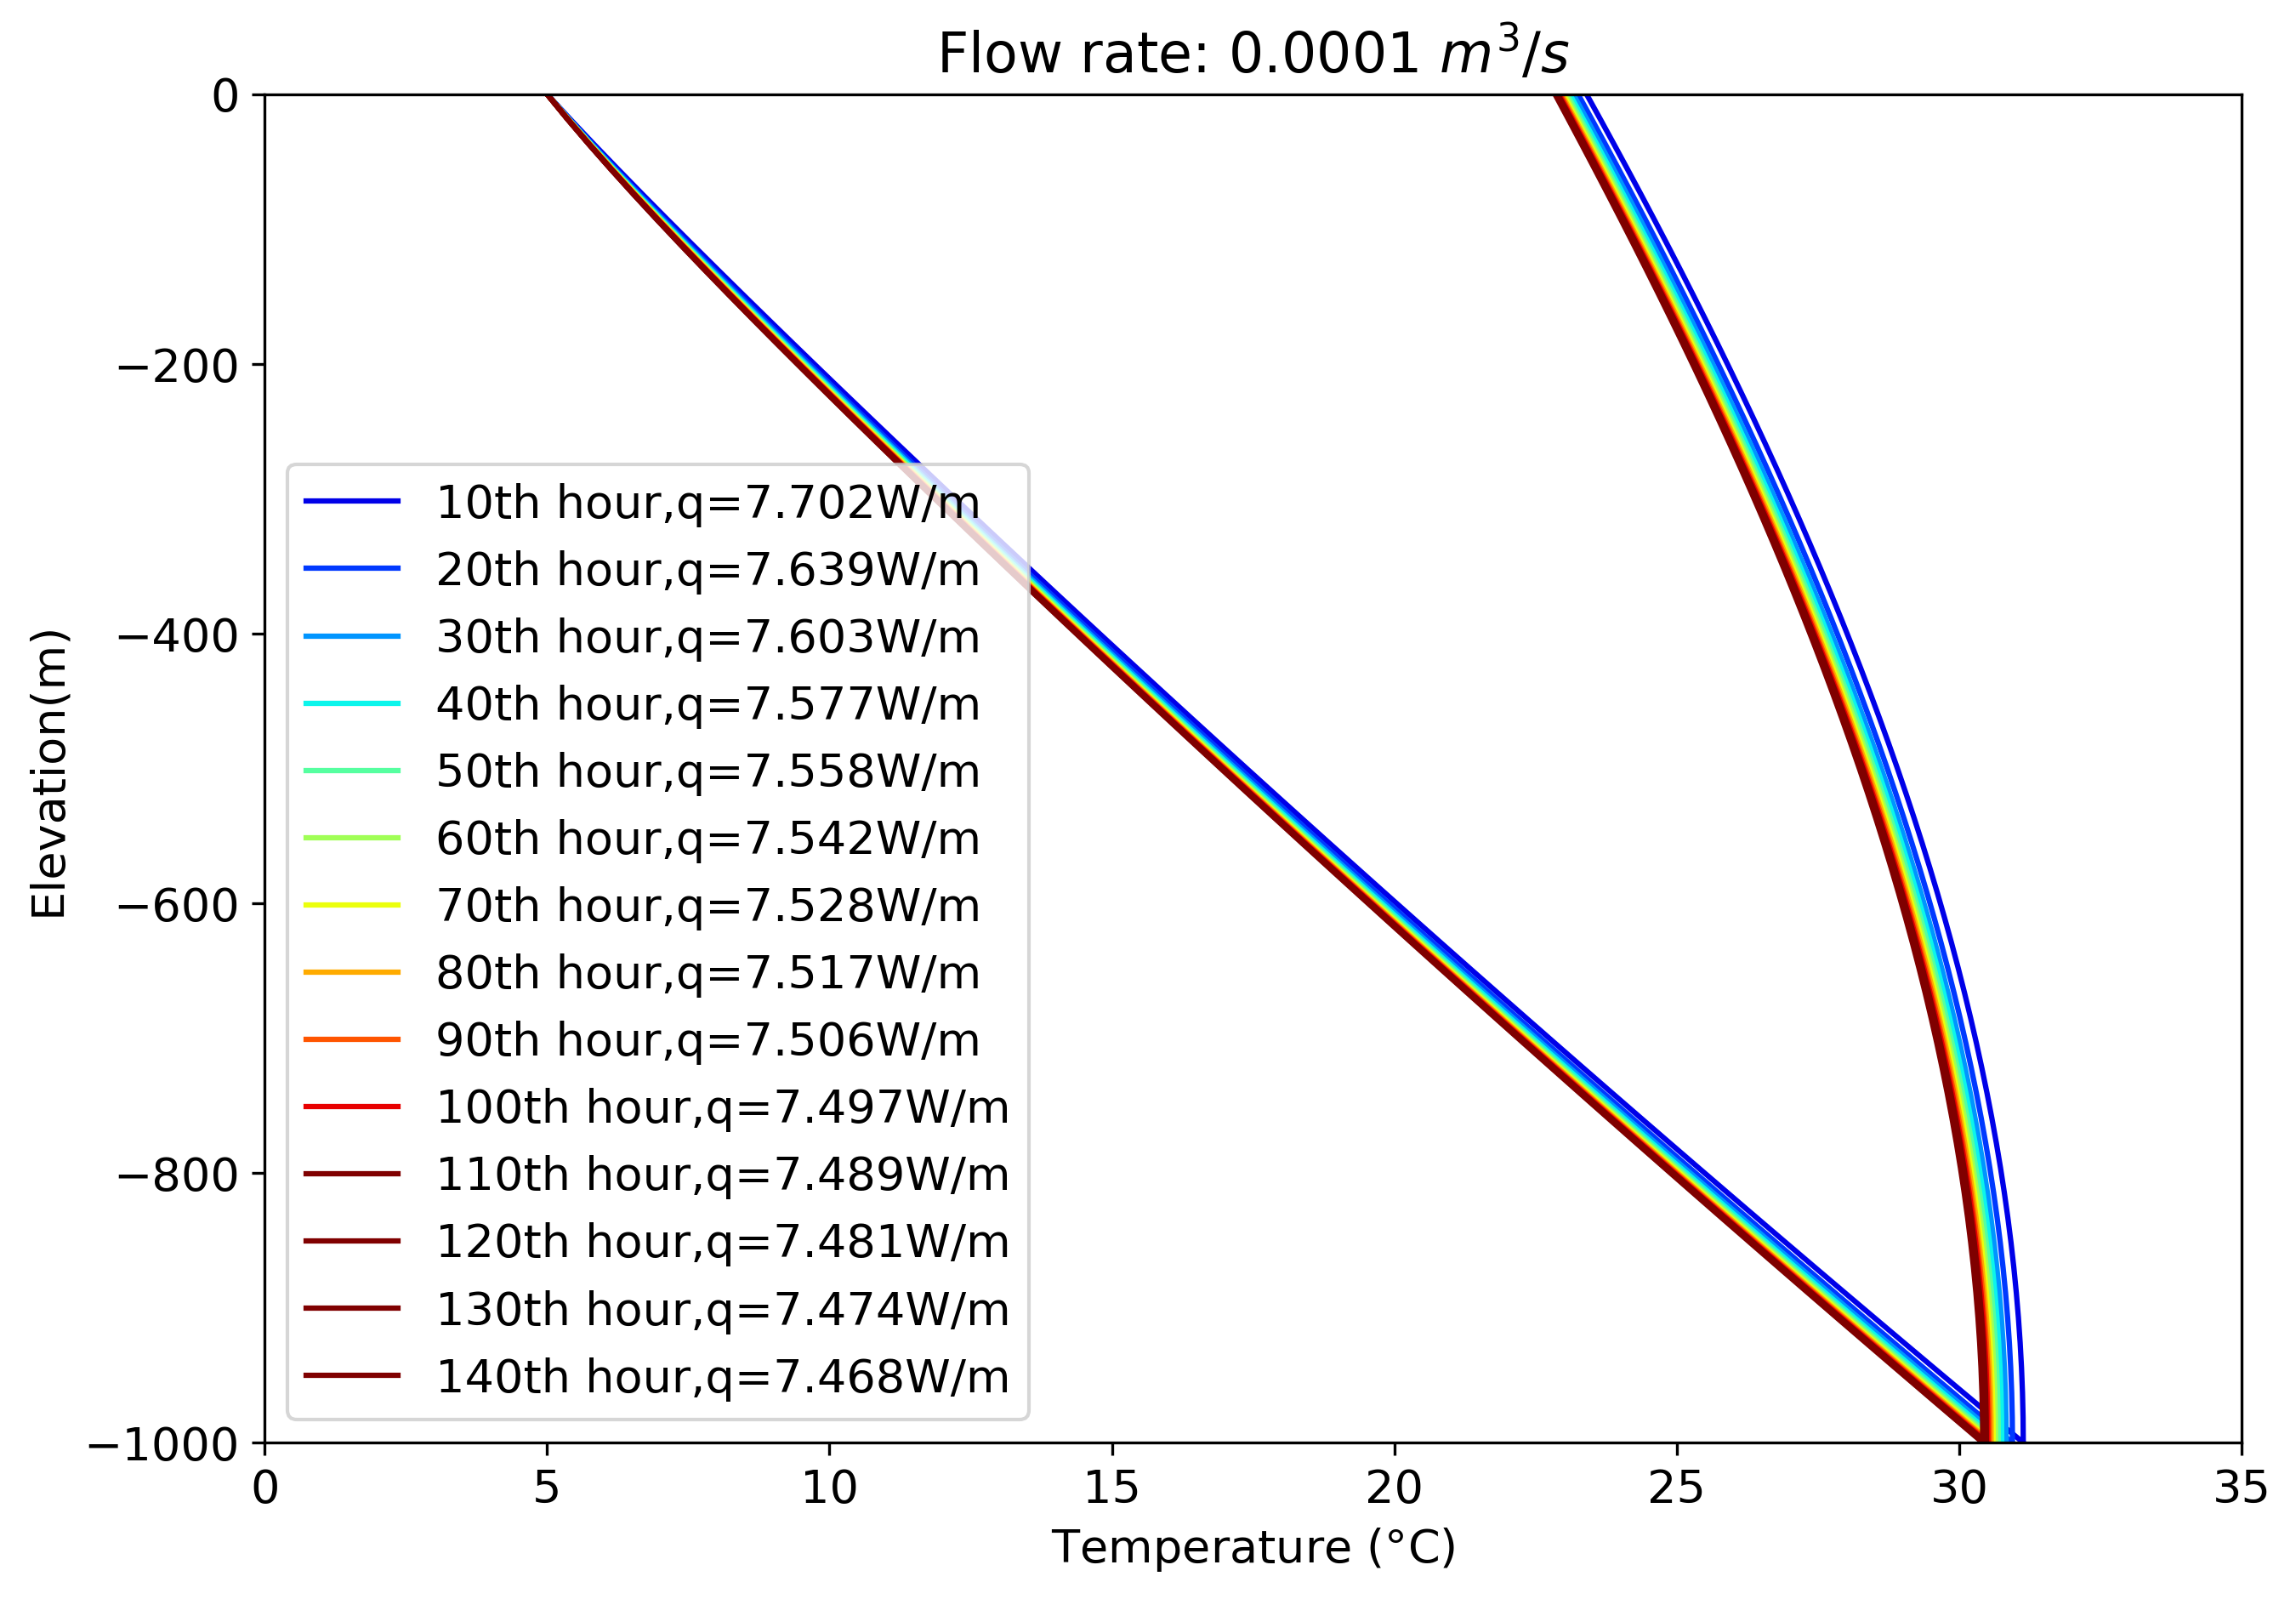
\includegraphics[width=0.48\textwidth]{Hours_1e-4_1000.png}
            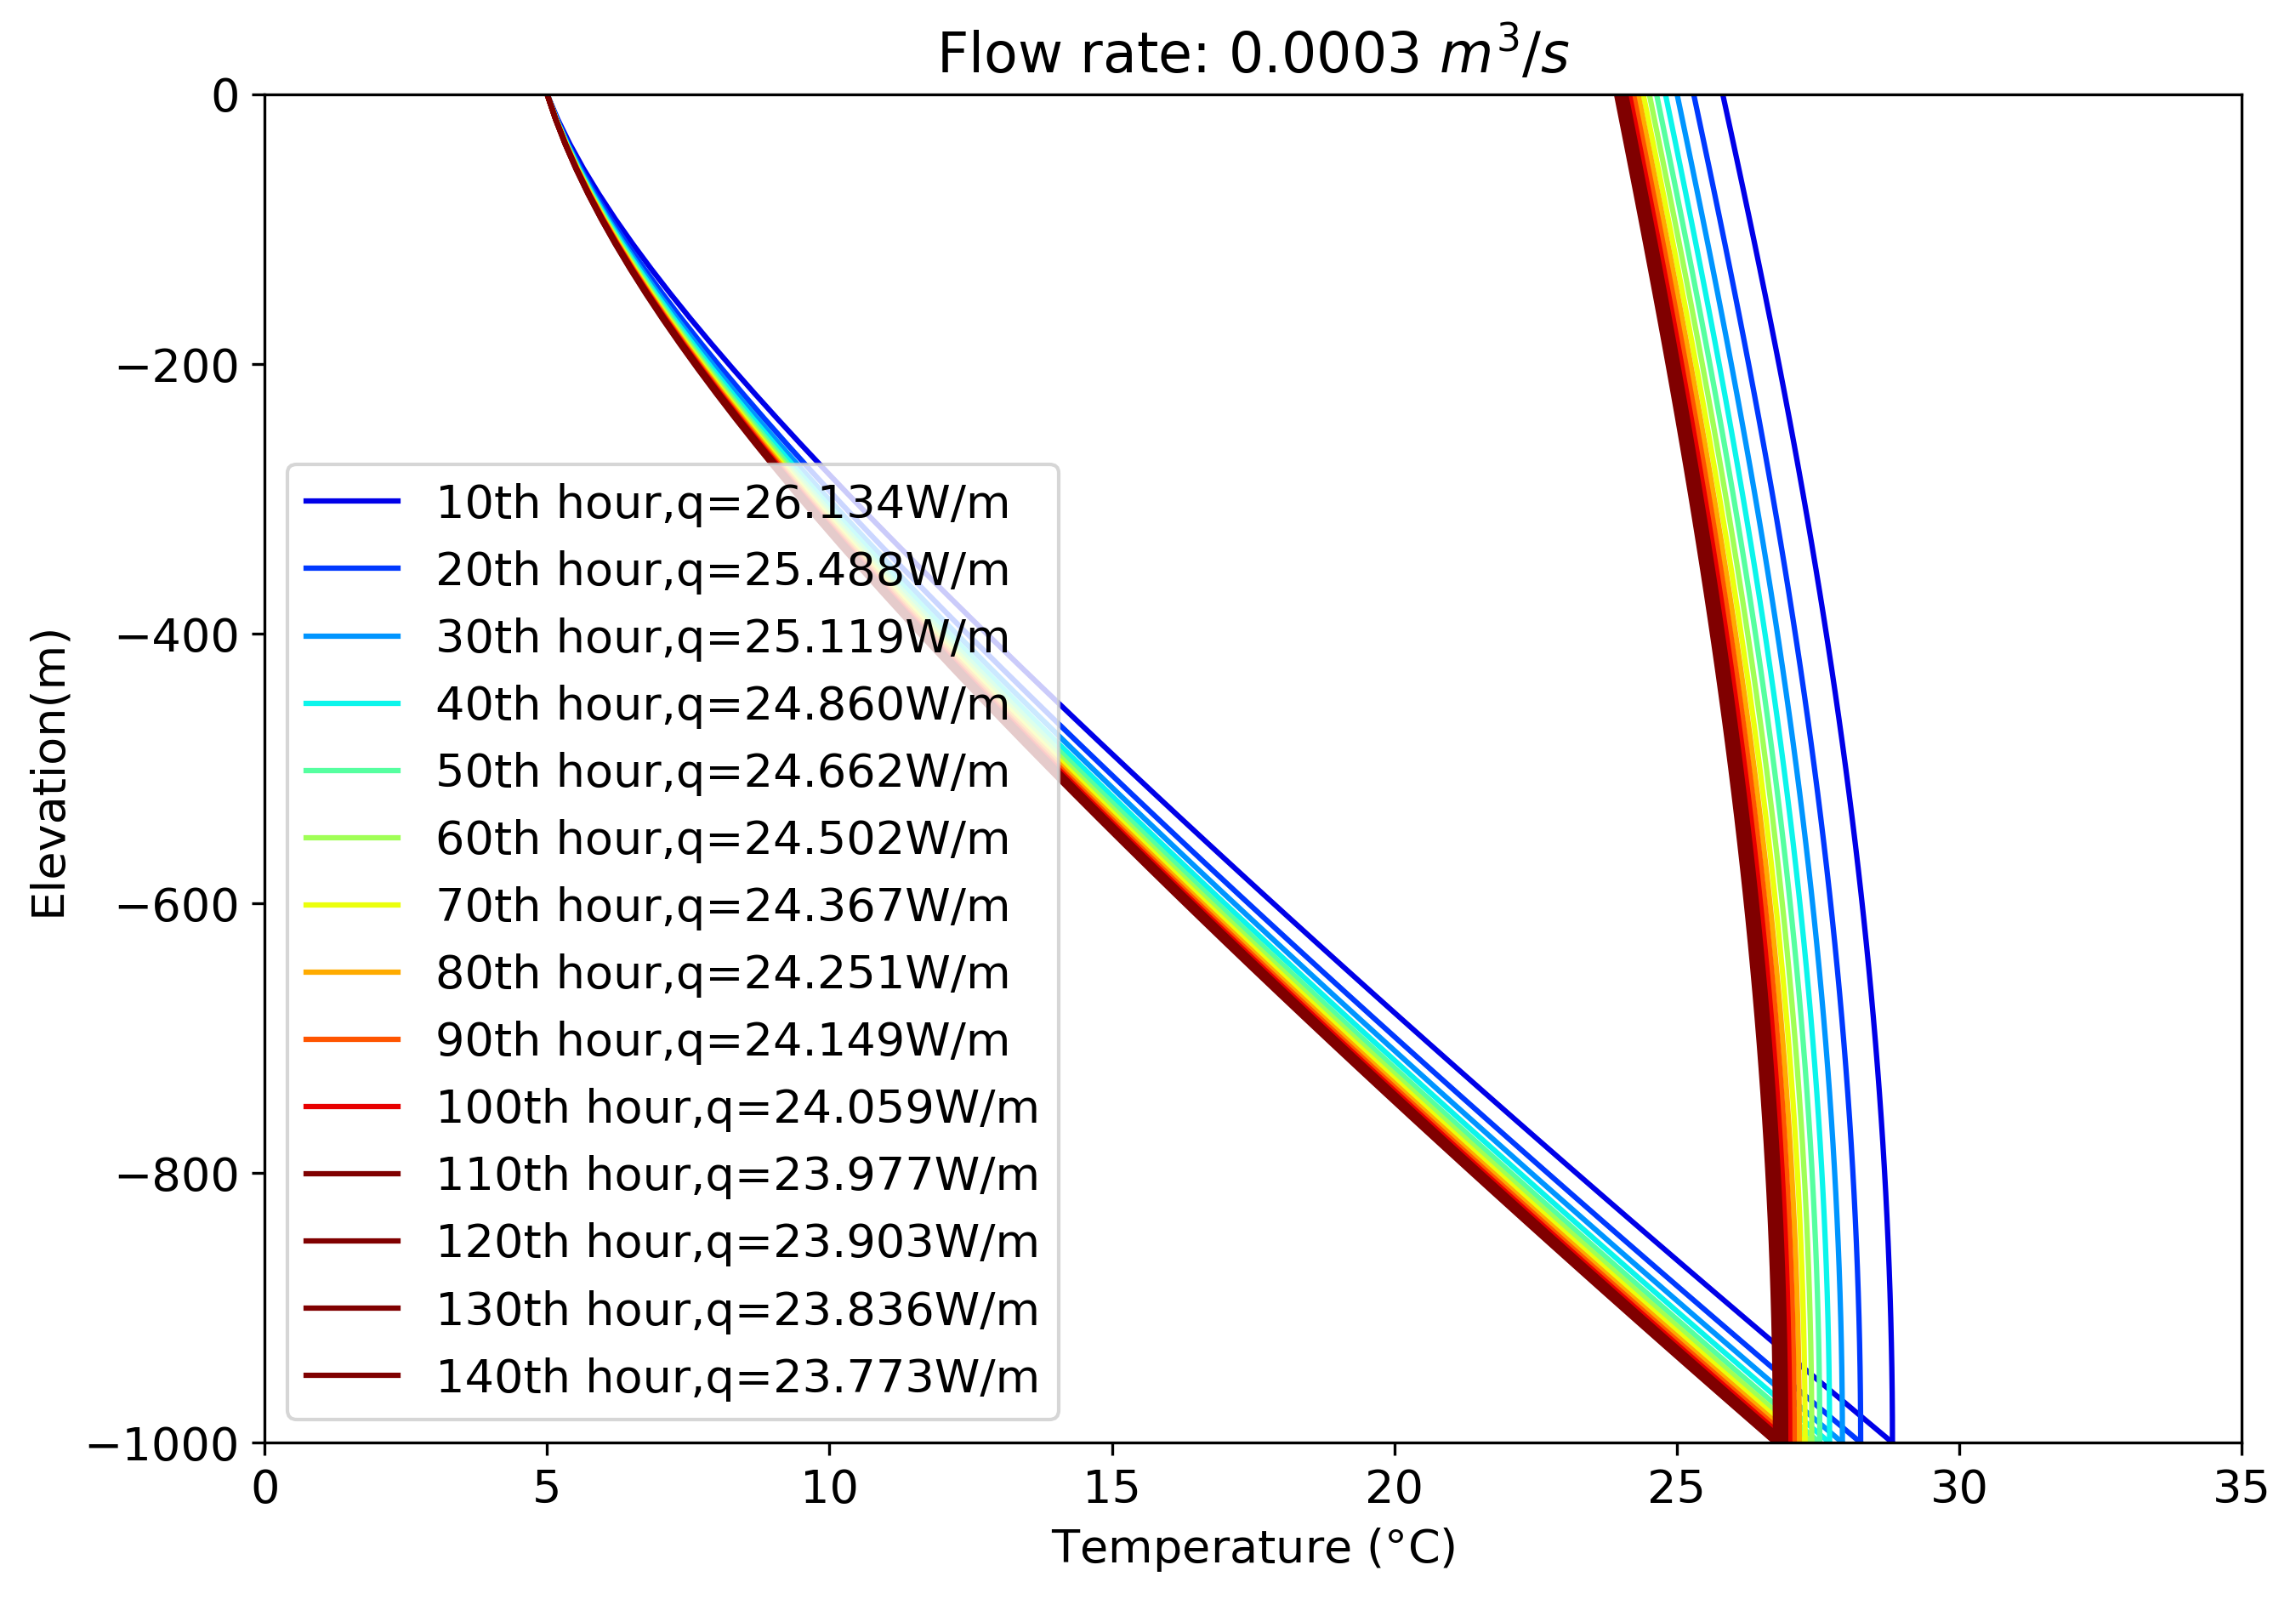
\includegraphics[width=0.48\textwidth]{Hours_3e-4_1000.png}
            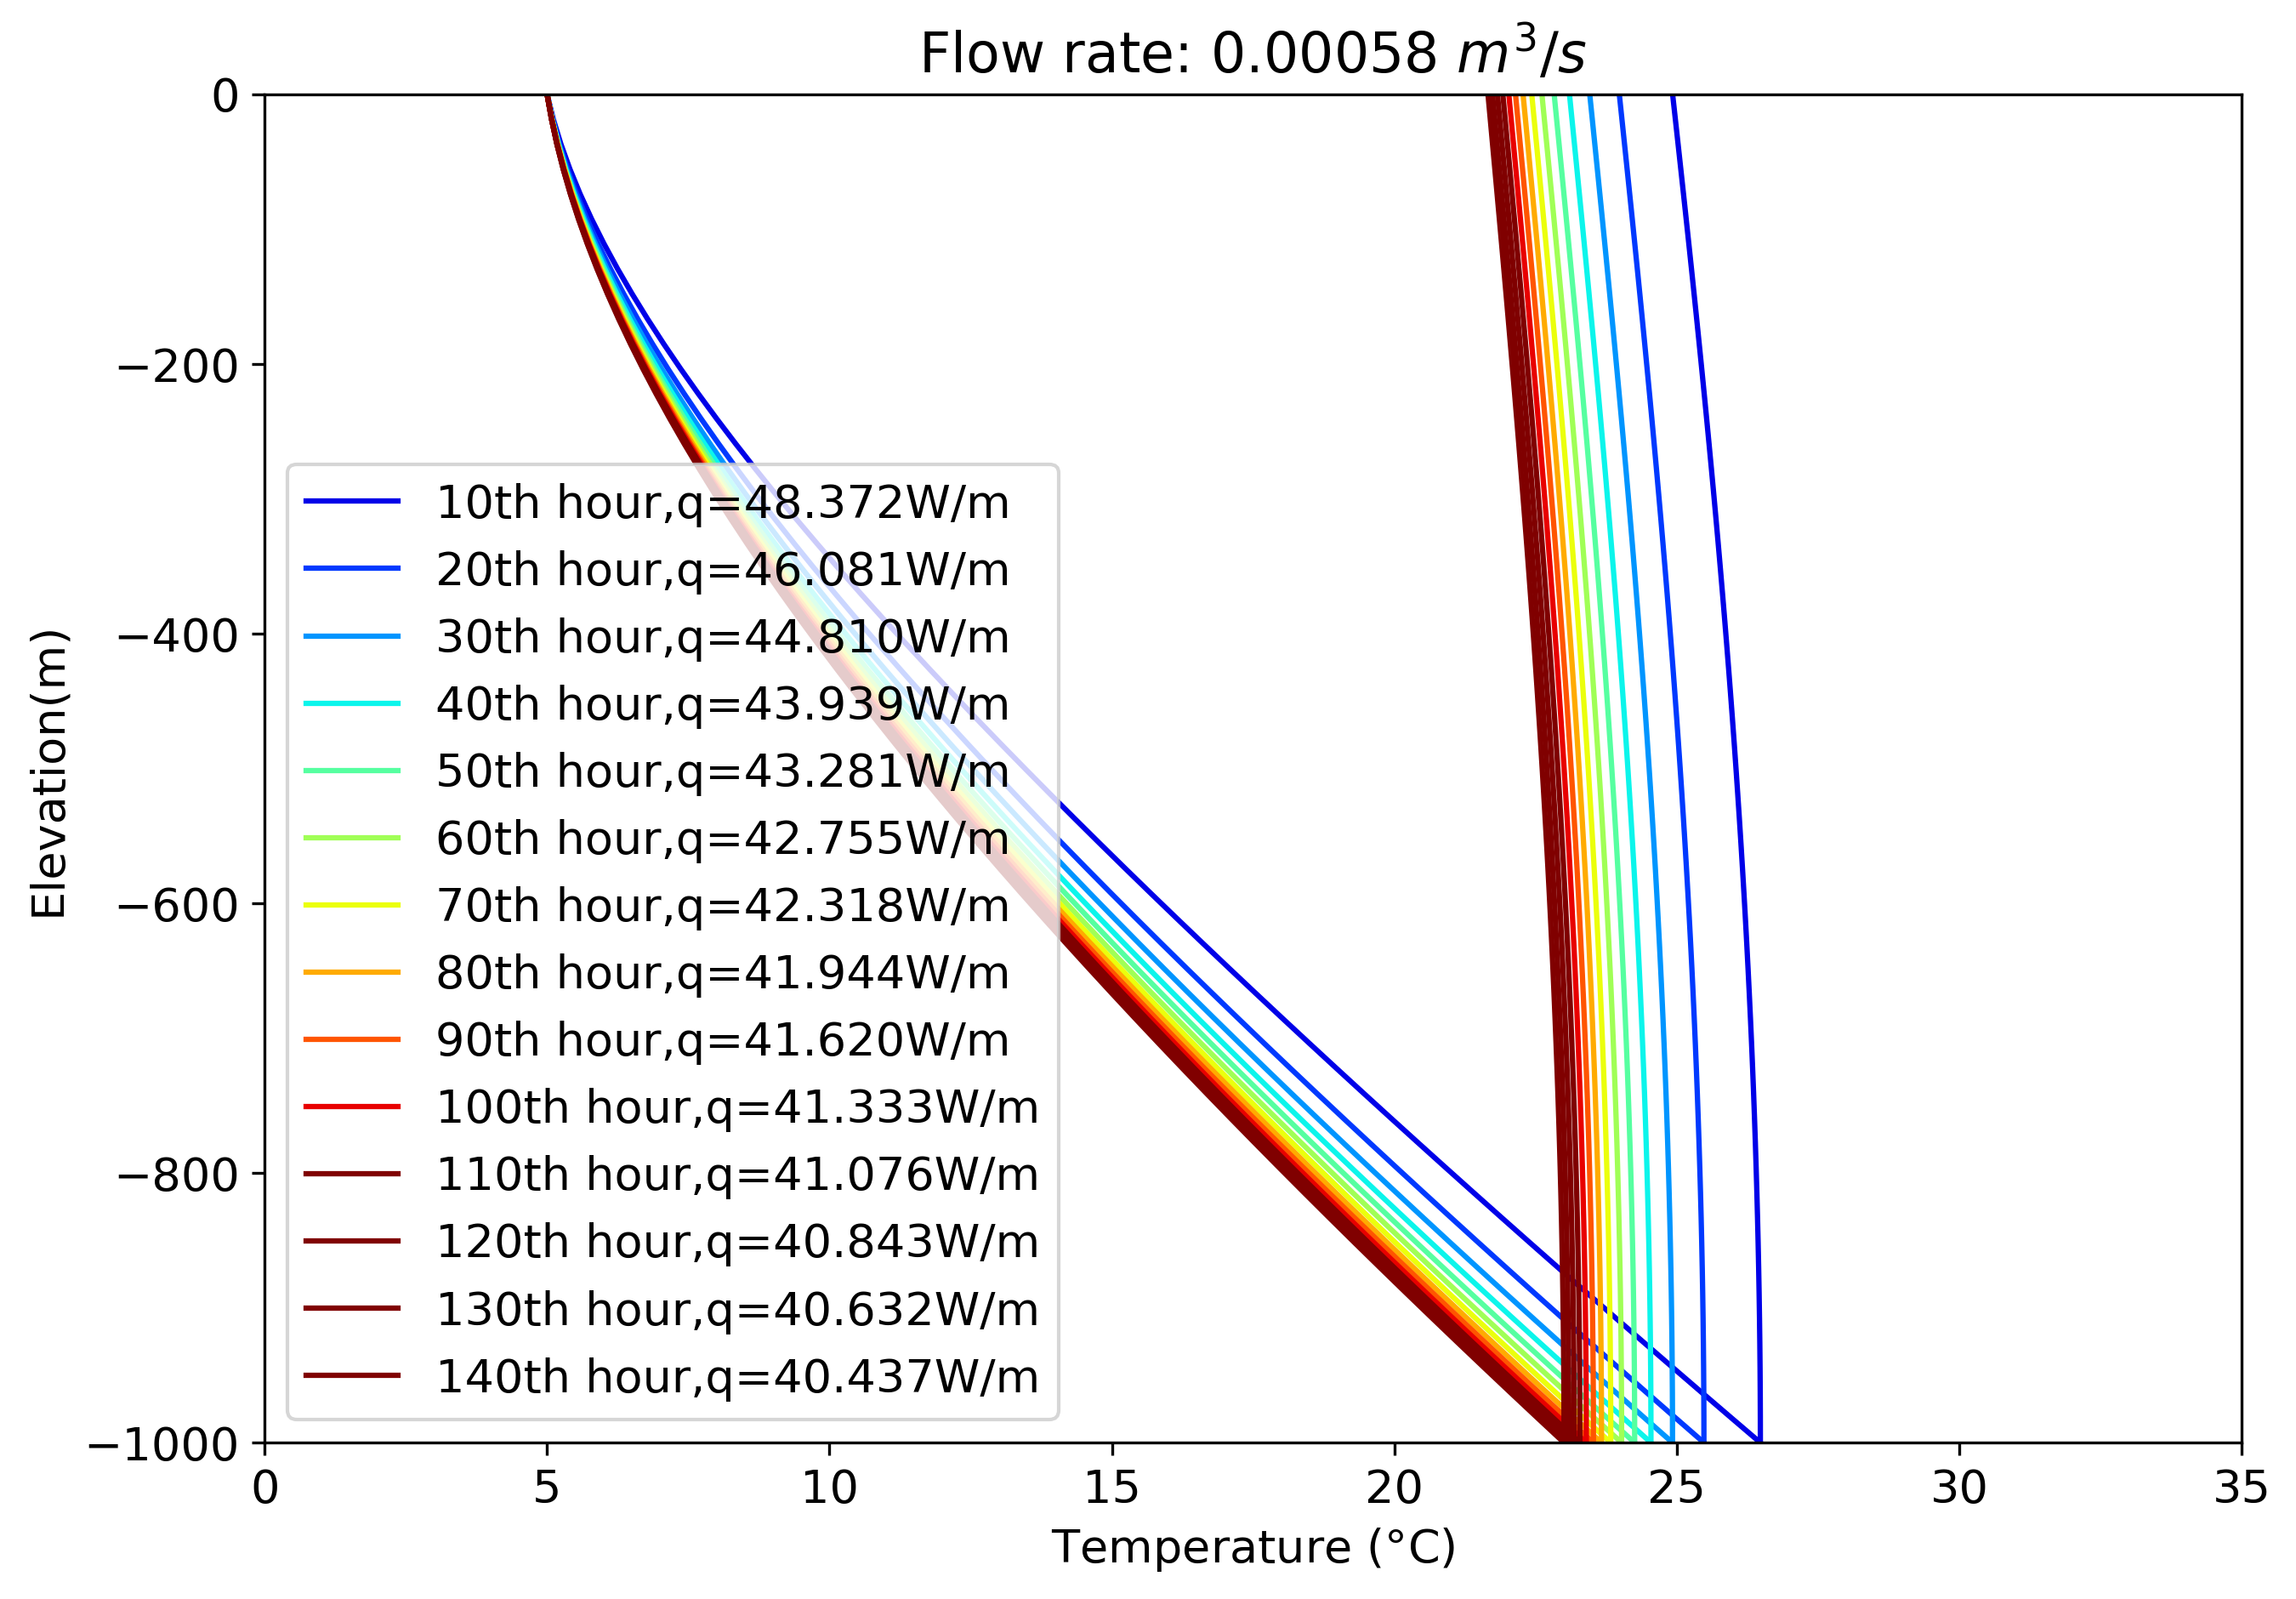
\includegraphics[width=0.48\textwidth]{Hours_Best58e-4_1000.png}
            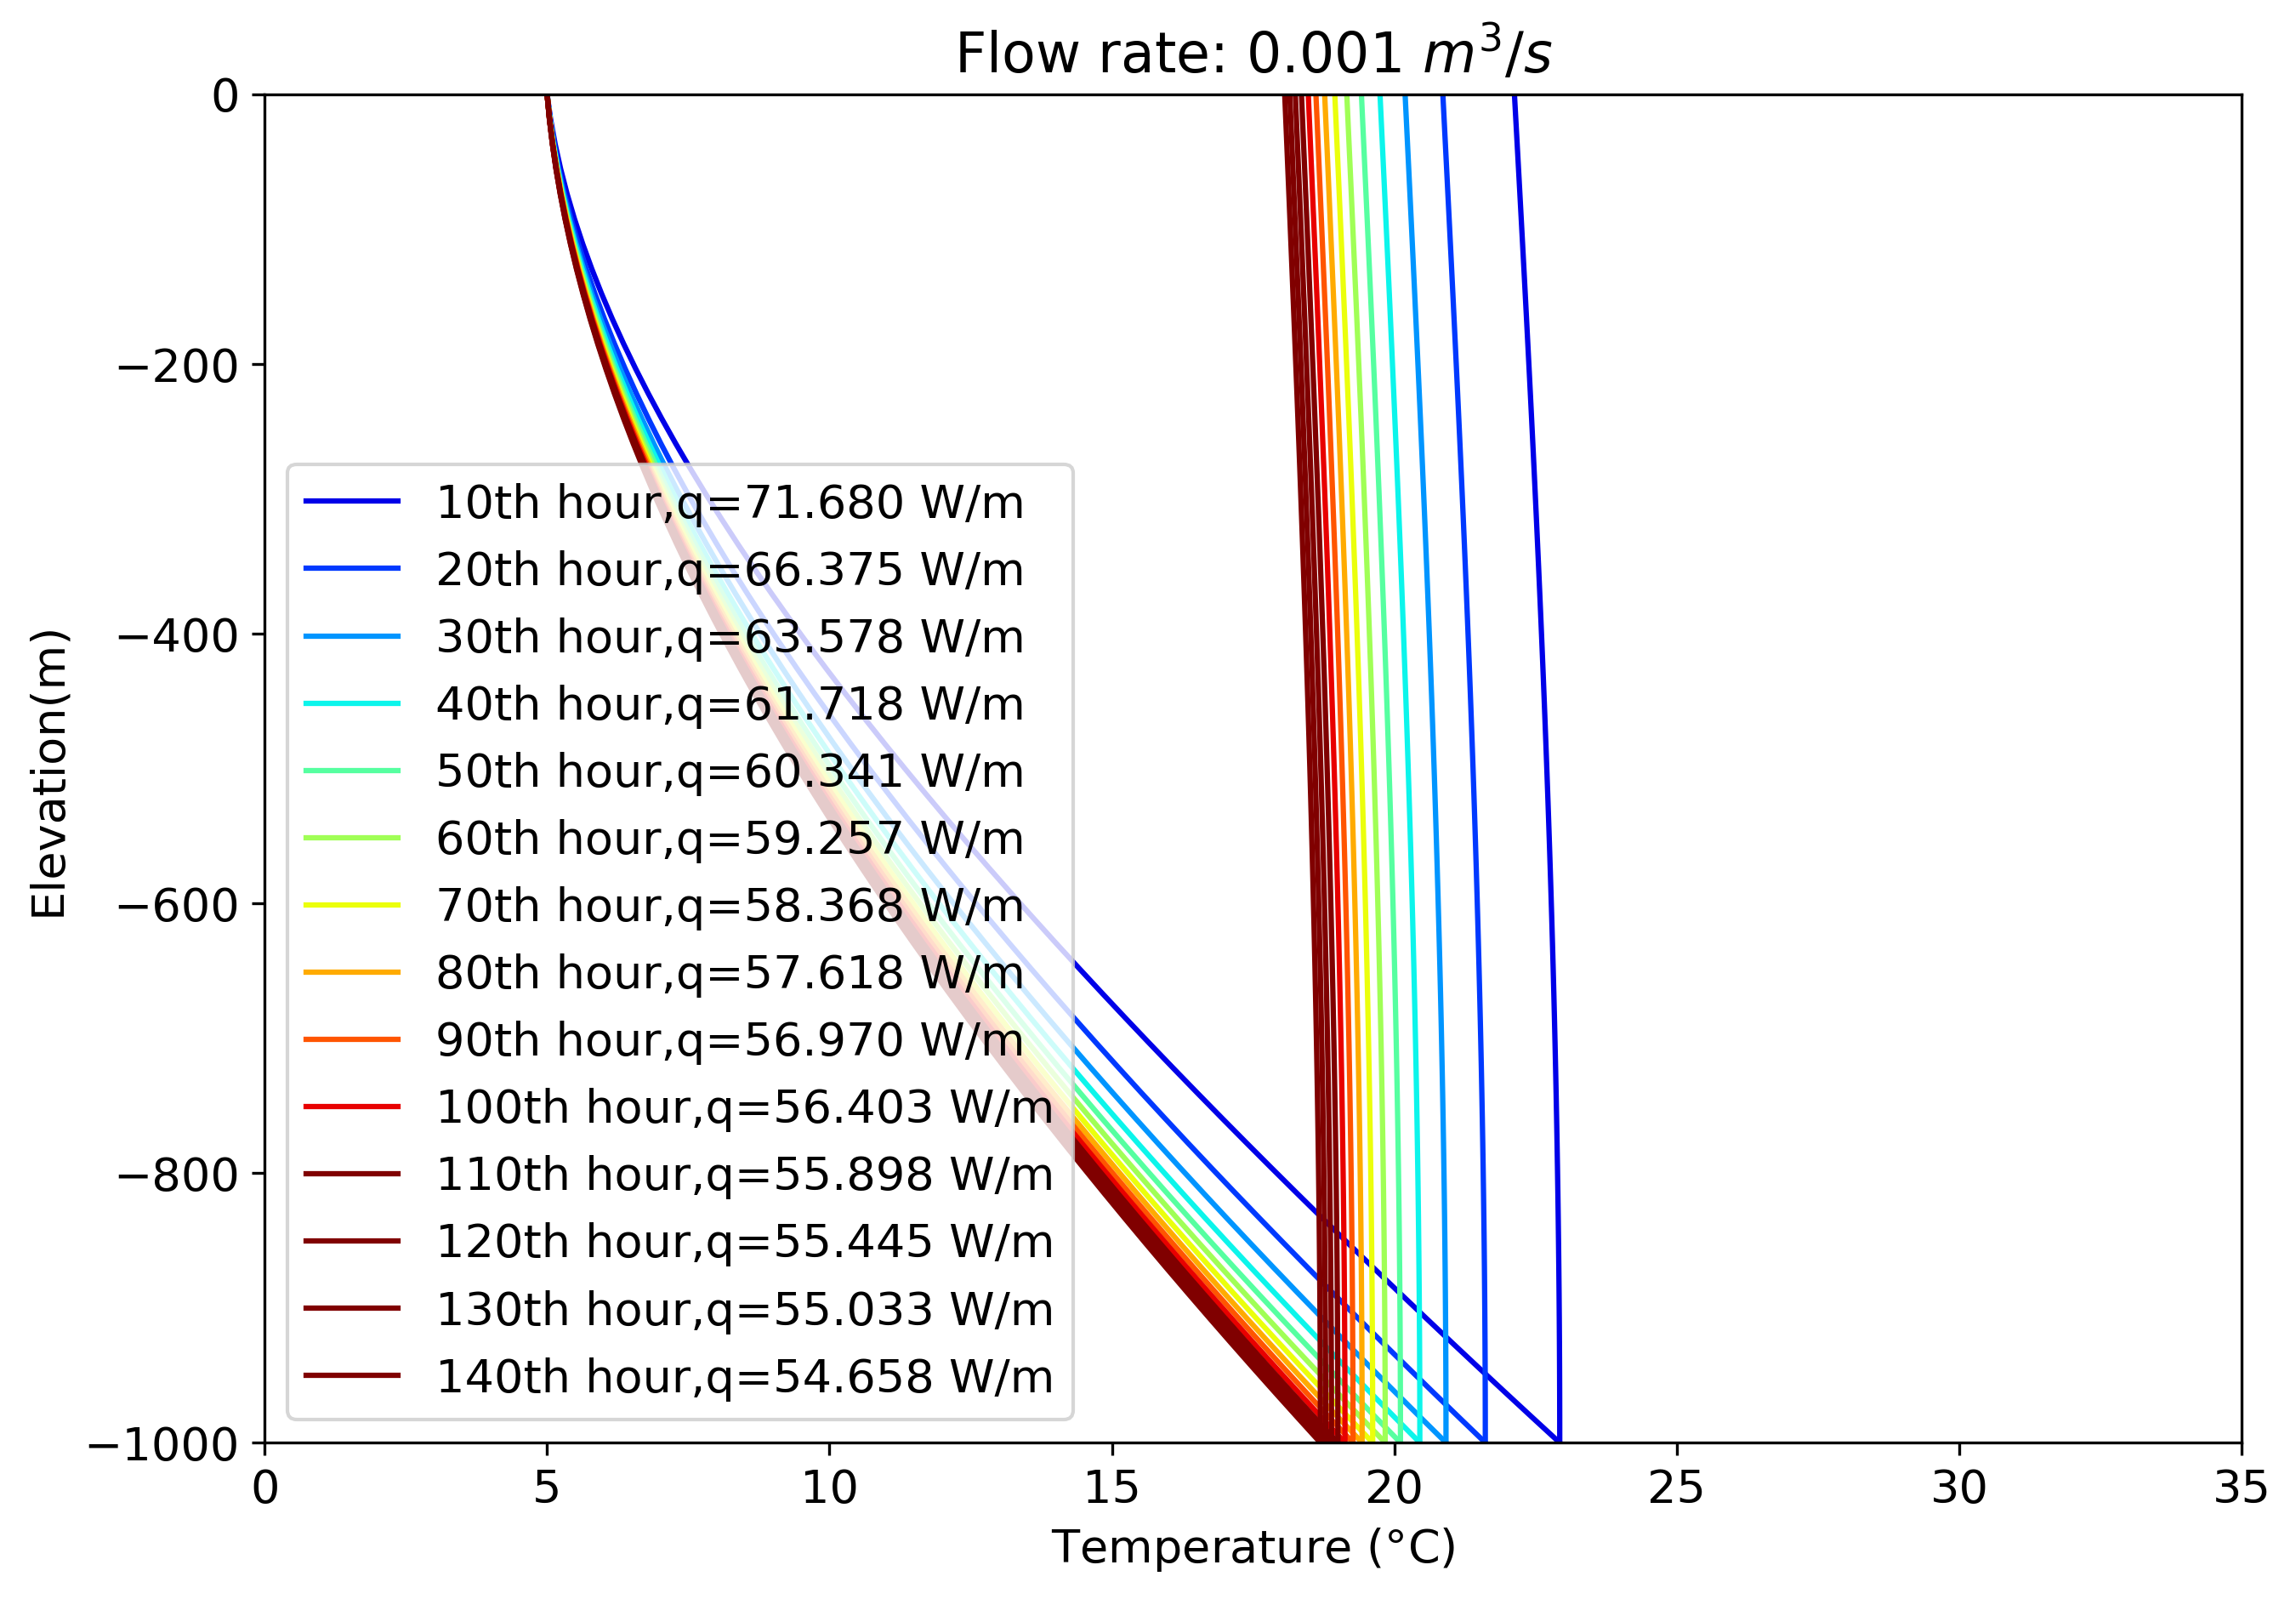
\includegraphics[width=0.48\textwidth]{Hours_1e-3_1000.png}
            \caption{Vertical temperature distribution and its variation over time for different flow rates: $w=0.0001 m^3/s$(top left), $w=0.0003 m^3/s$(top right),$w=0.00058 m^3/s$ (bottom left),$w=0.001 m^3/s$ (bottom right).}
            \label{fig:FR3_dev}
        \end{figure}
        
		To better illustrate how the heat extraction rate changes over time, we plotted the heat extraction rate of the 1st 1000 hours as shown in Figure 10. As all the heat extraction rate gradually falls lower, the model yields a relatively steady heat extraction rate for all six flow rates. The increase from the flow rate of 0.00058 $m^3/s$ to 0.001 $m^3/s$ results in a limited increase of heat extraction rate of less 5\%. Since increasing the flow rate will also increase the pumping cost for the operation, this small increase of heat extraction rate does not easily justify the increased operational costs. A more desirable flow rate is, therefore, set at 0.001 $m^3/s$ to achieve better heat extraction rate, but at a smaller flow rate and therefore smaller necessary pumping power for further analysis. The temperature out for this remains steady at approximately 18.5 \degree C, which could be desirable for a high-COP GSHP, but not suitable yet for direct heating.
        \begin{figure}[h!]
            \centering
            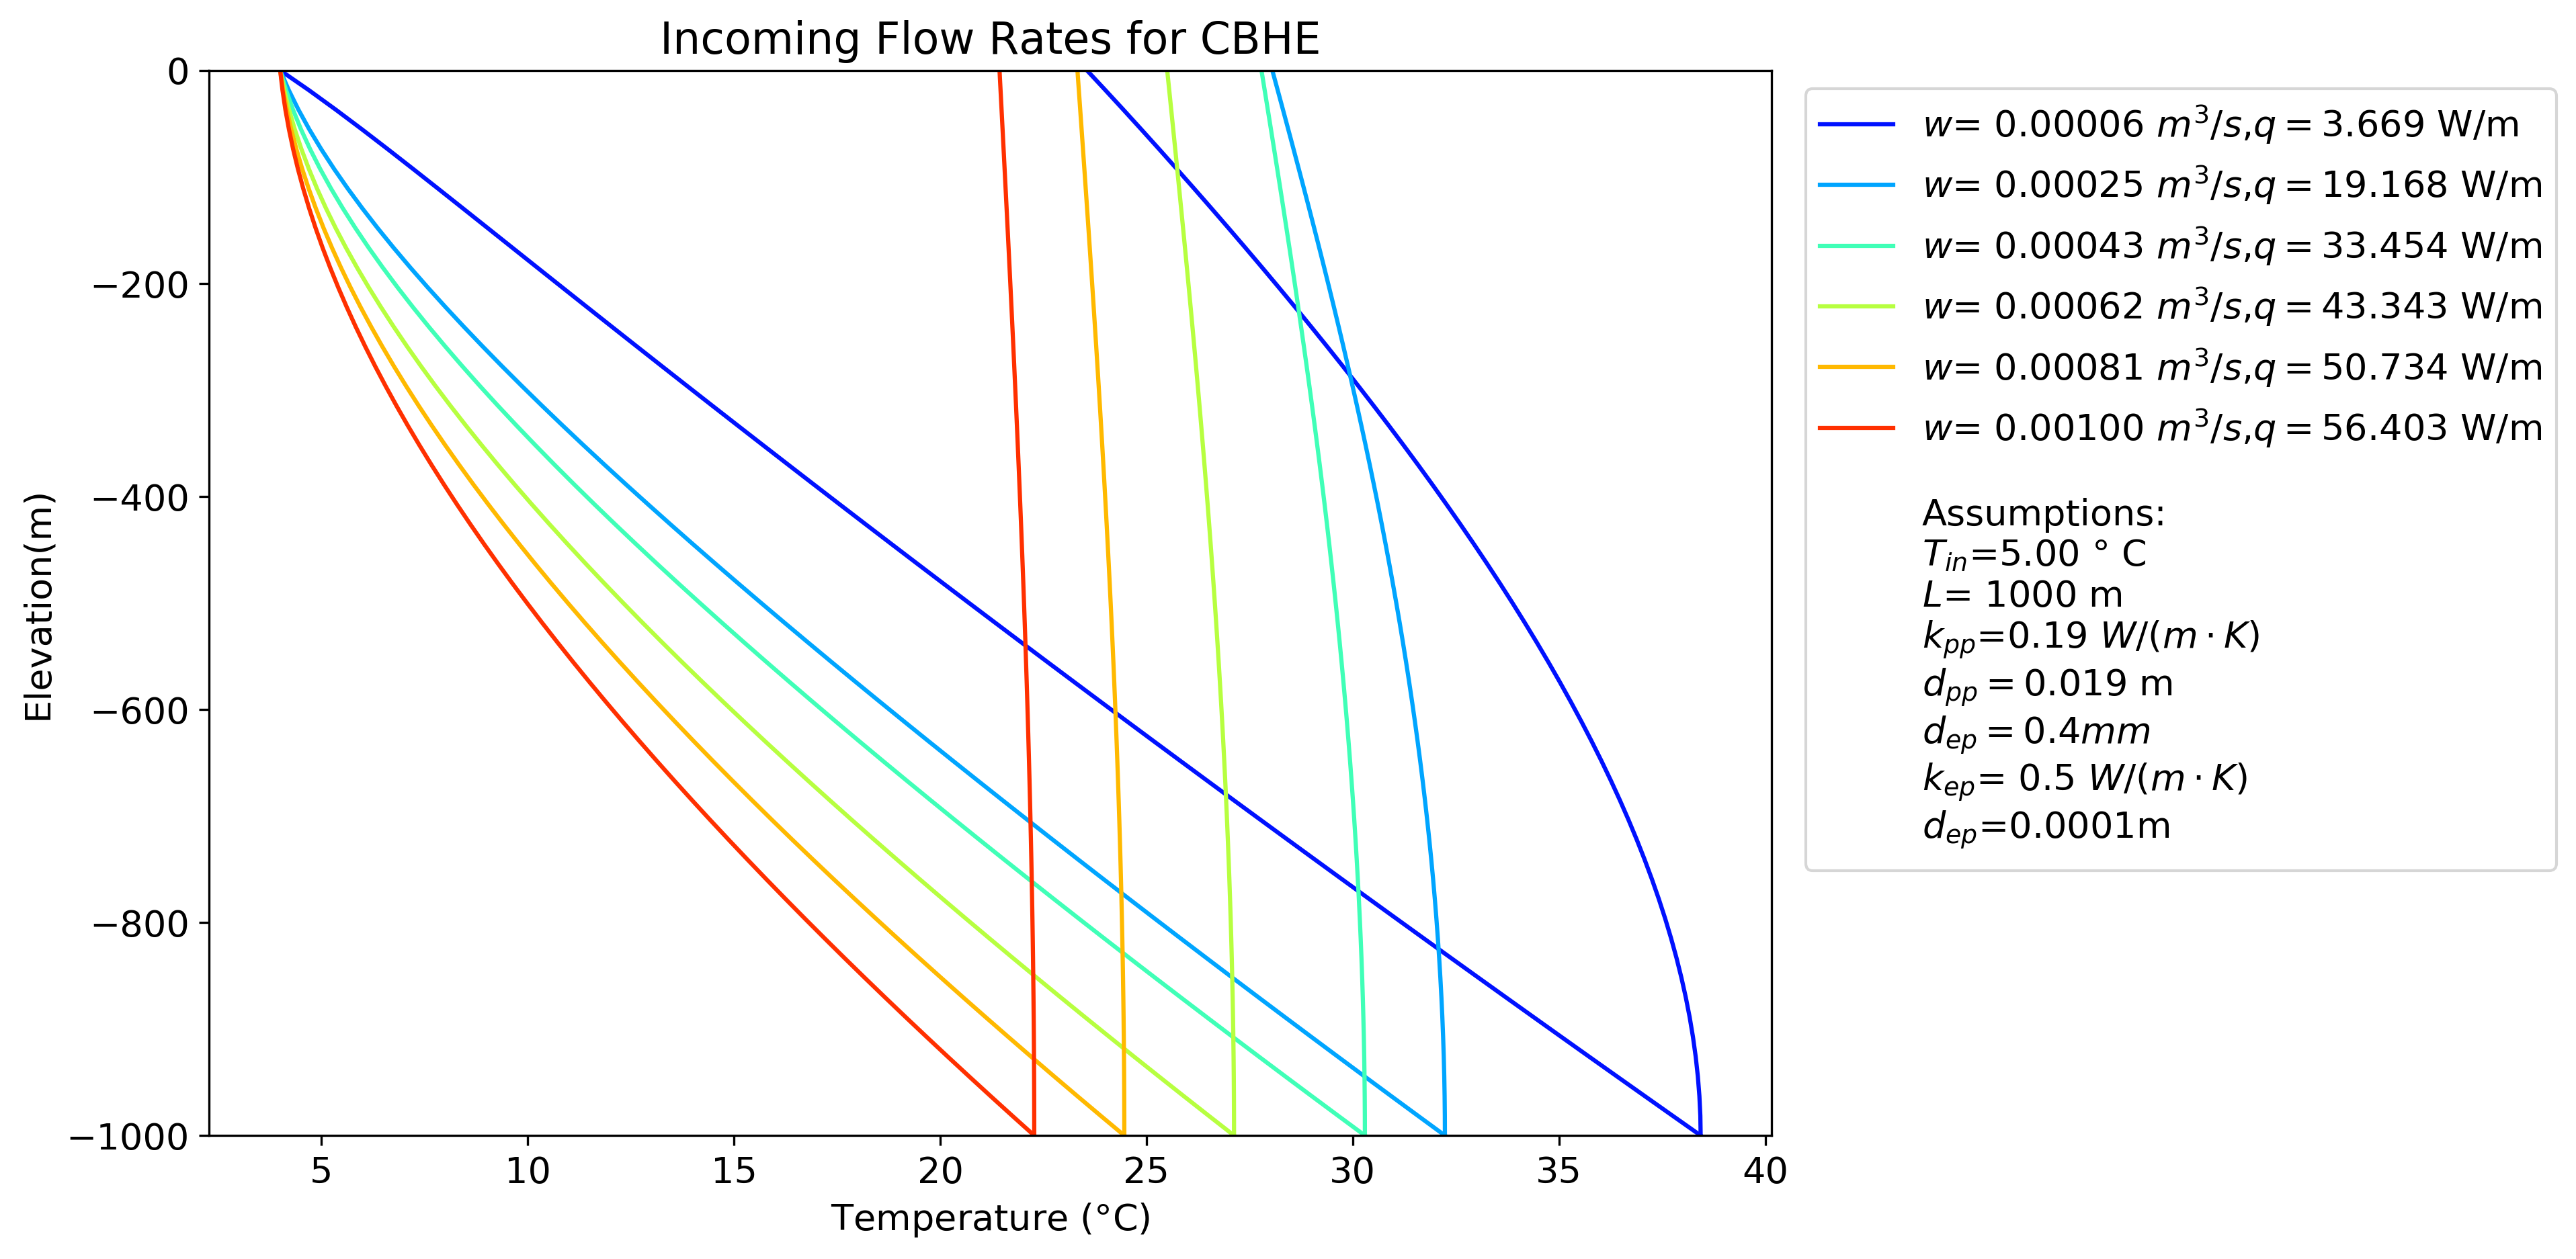
\includegraphics[width=0.75\textwidth]{fr_1000_MIN.png}
            \caption{Vertical temperature distribution and heat extraction rate at 100th hour}
            \label{fig:frs}
        \end{figure}
        
        \begin{figure}[h!]
            \centering
            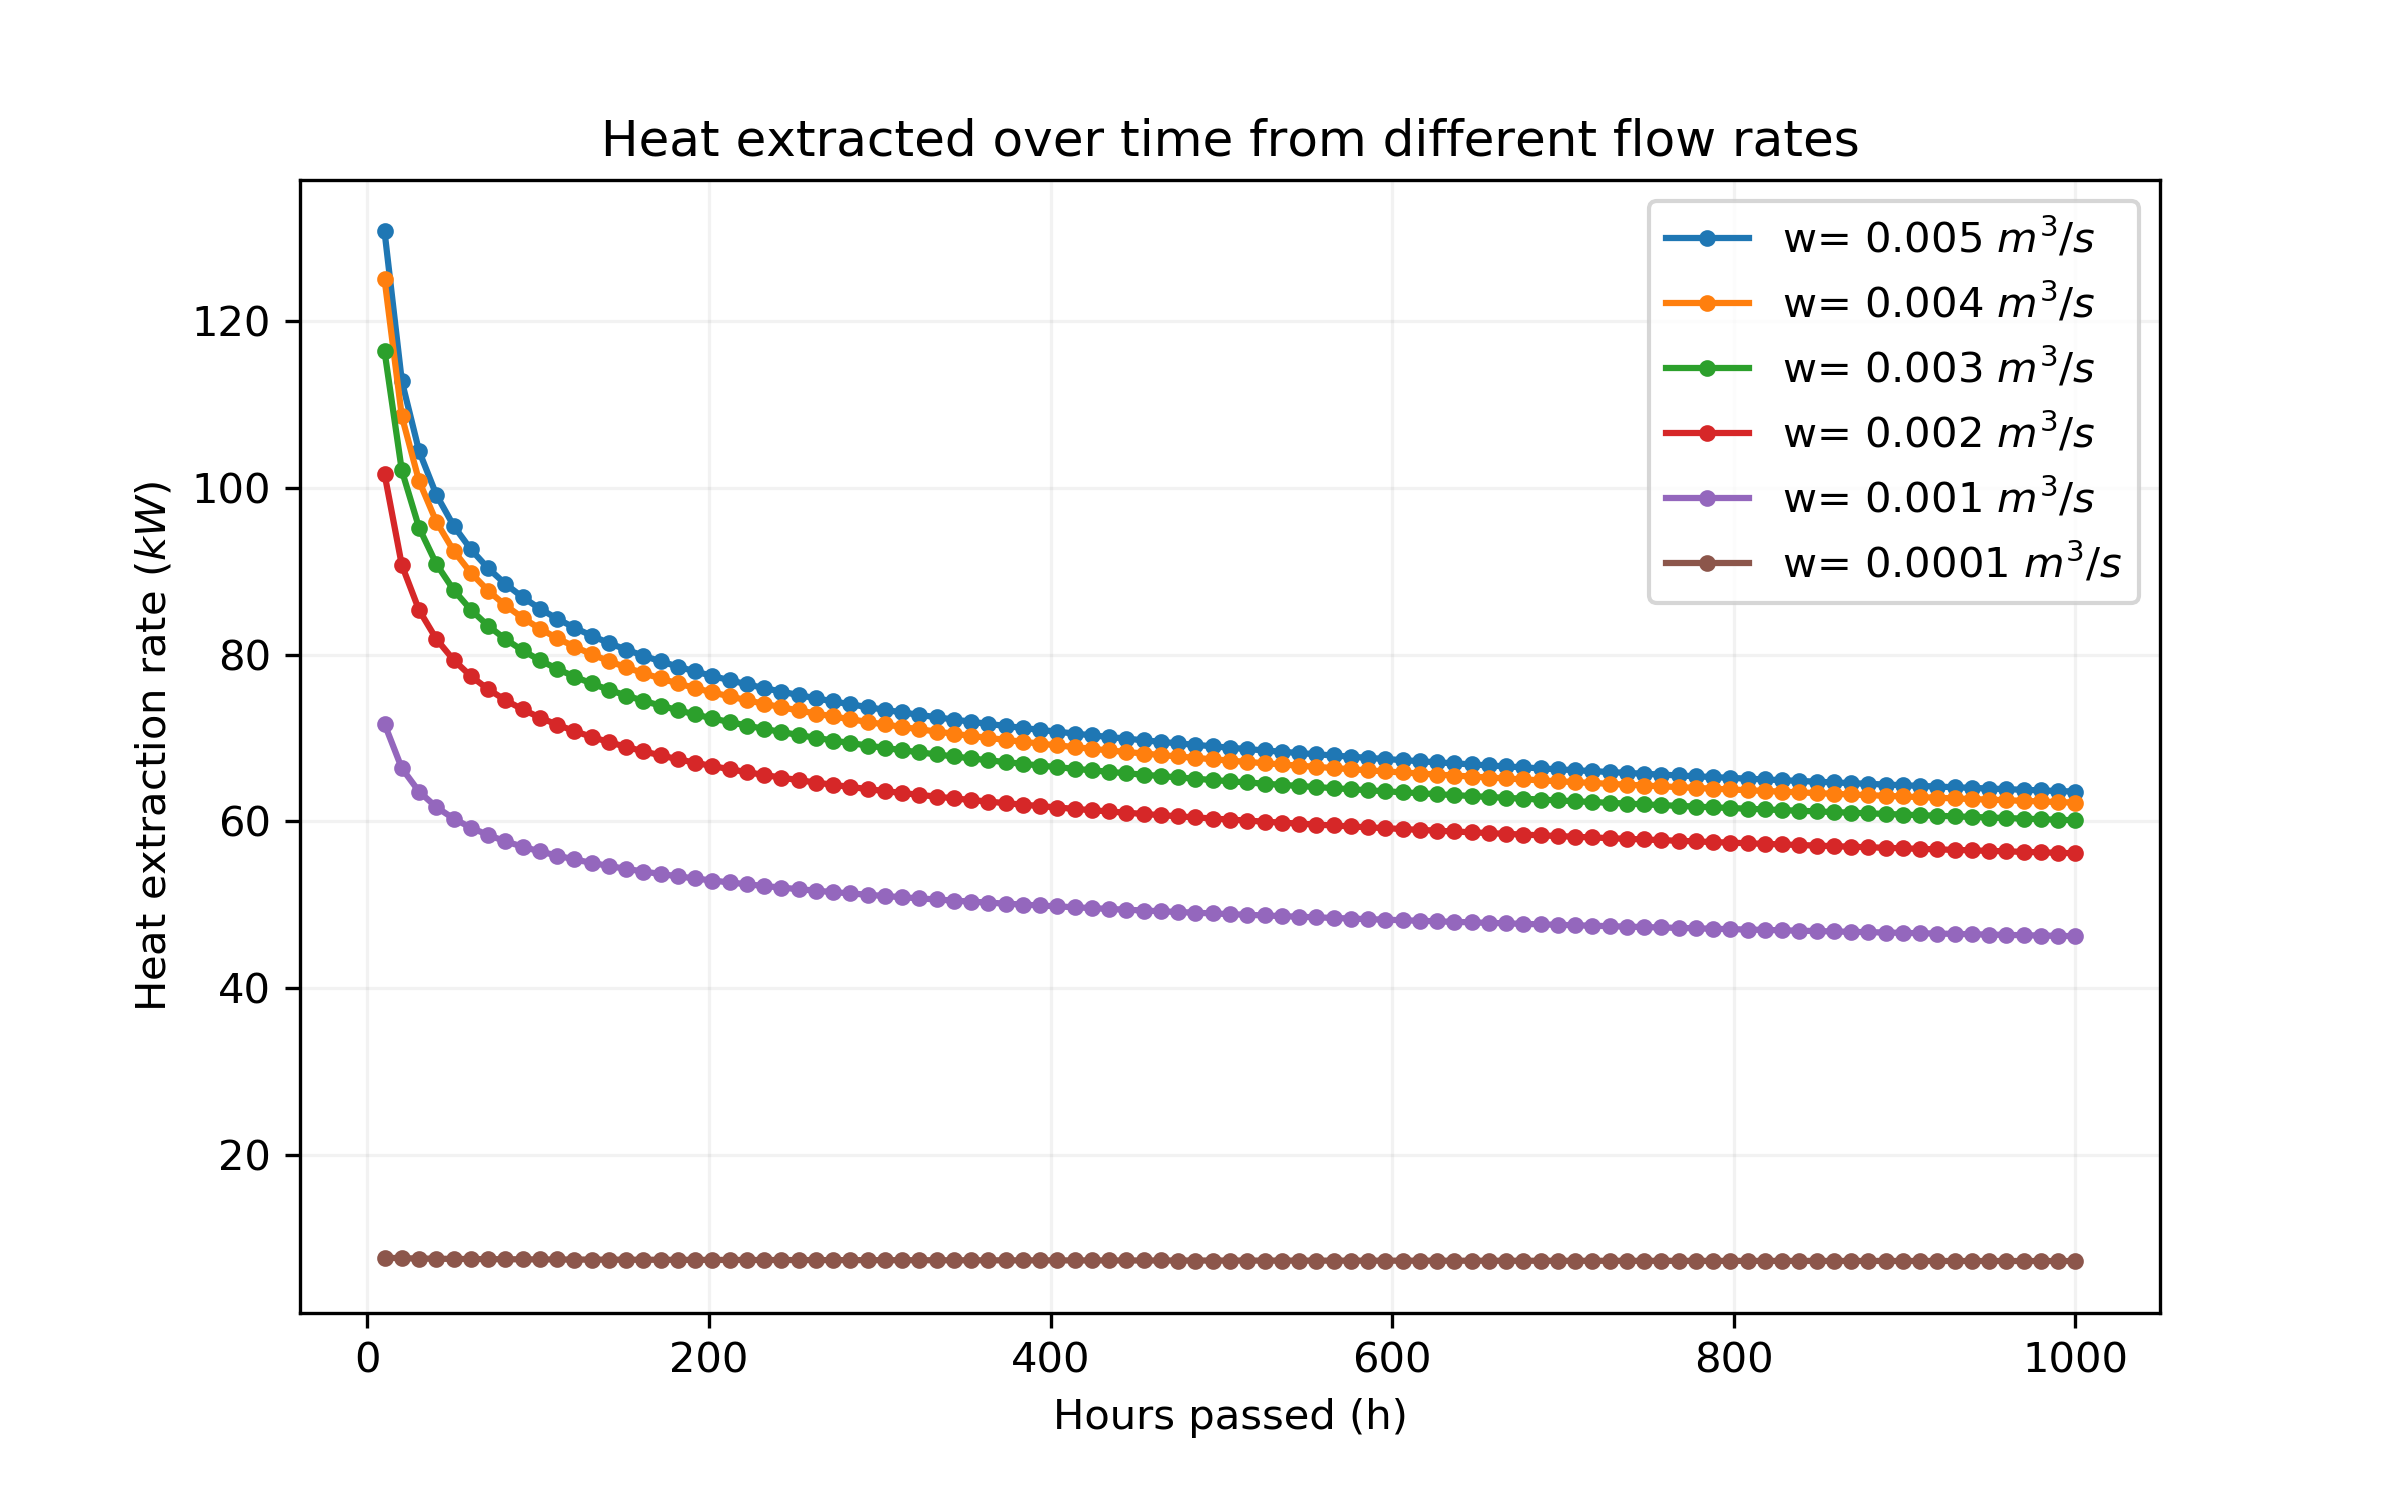
\includegraphics[width=0.75\textwidth]{HeatExtractHours.png}
            \caption{Heat extraction rate variation over 1000 hours for different flow rates.}
            \label{fig:frHR}
        \end{figure}    
	\subsubsection{Site-specific variables}
		For site-specific variables, we examined the geothermal gradient and the thermal conductivity of potential sites. 
		
		%Also compare different Rb? Would this be an interesting thing to compare? I'd think so I hope??? Just generate a bunch of Rb and compre them.
		Ultimately, we compared the resulting $R_b$ of all the cases we investigated and plot them as a scattered plot to indicate the range of variations that may result in performance differences between different CBHEs. 
		
		\subsubsection{Geothermal gradient}
		The two non-design parameters, depth and thermal conductivity of the soil can also be examined, and provide some preliminary understanding of how the original CBHE 	would have experienced heat extraction when the CBHE is in a different location with different environmental parameters. Setting the geothermal gradient at 1 Kelvin per 100 meters and 5 Kelvin per 100 meters, the 100th hour’s vertical temperature distribution for the CBHE with original configuration except for being 1000 meters deep can be found in Figure ~\ref{fig:GG}.
	    \begin{figure}[h!]
	        \centering
	        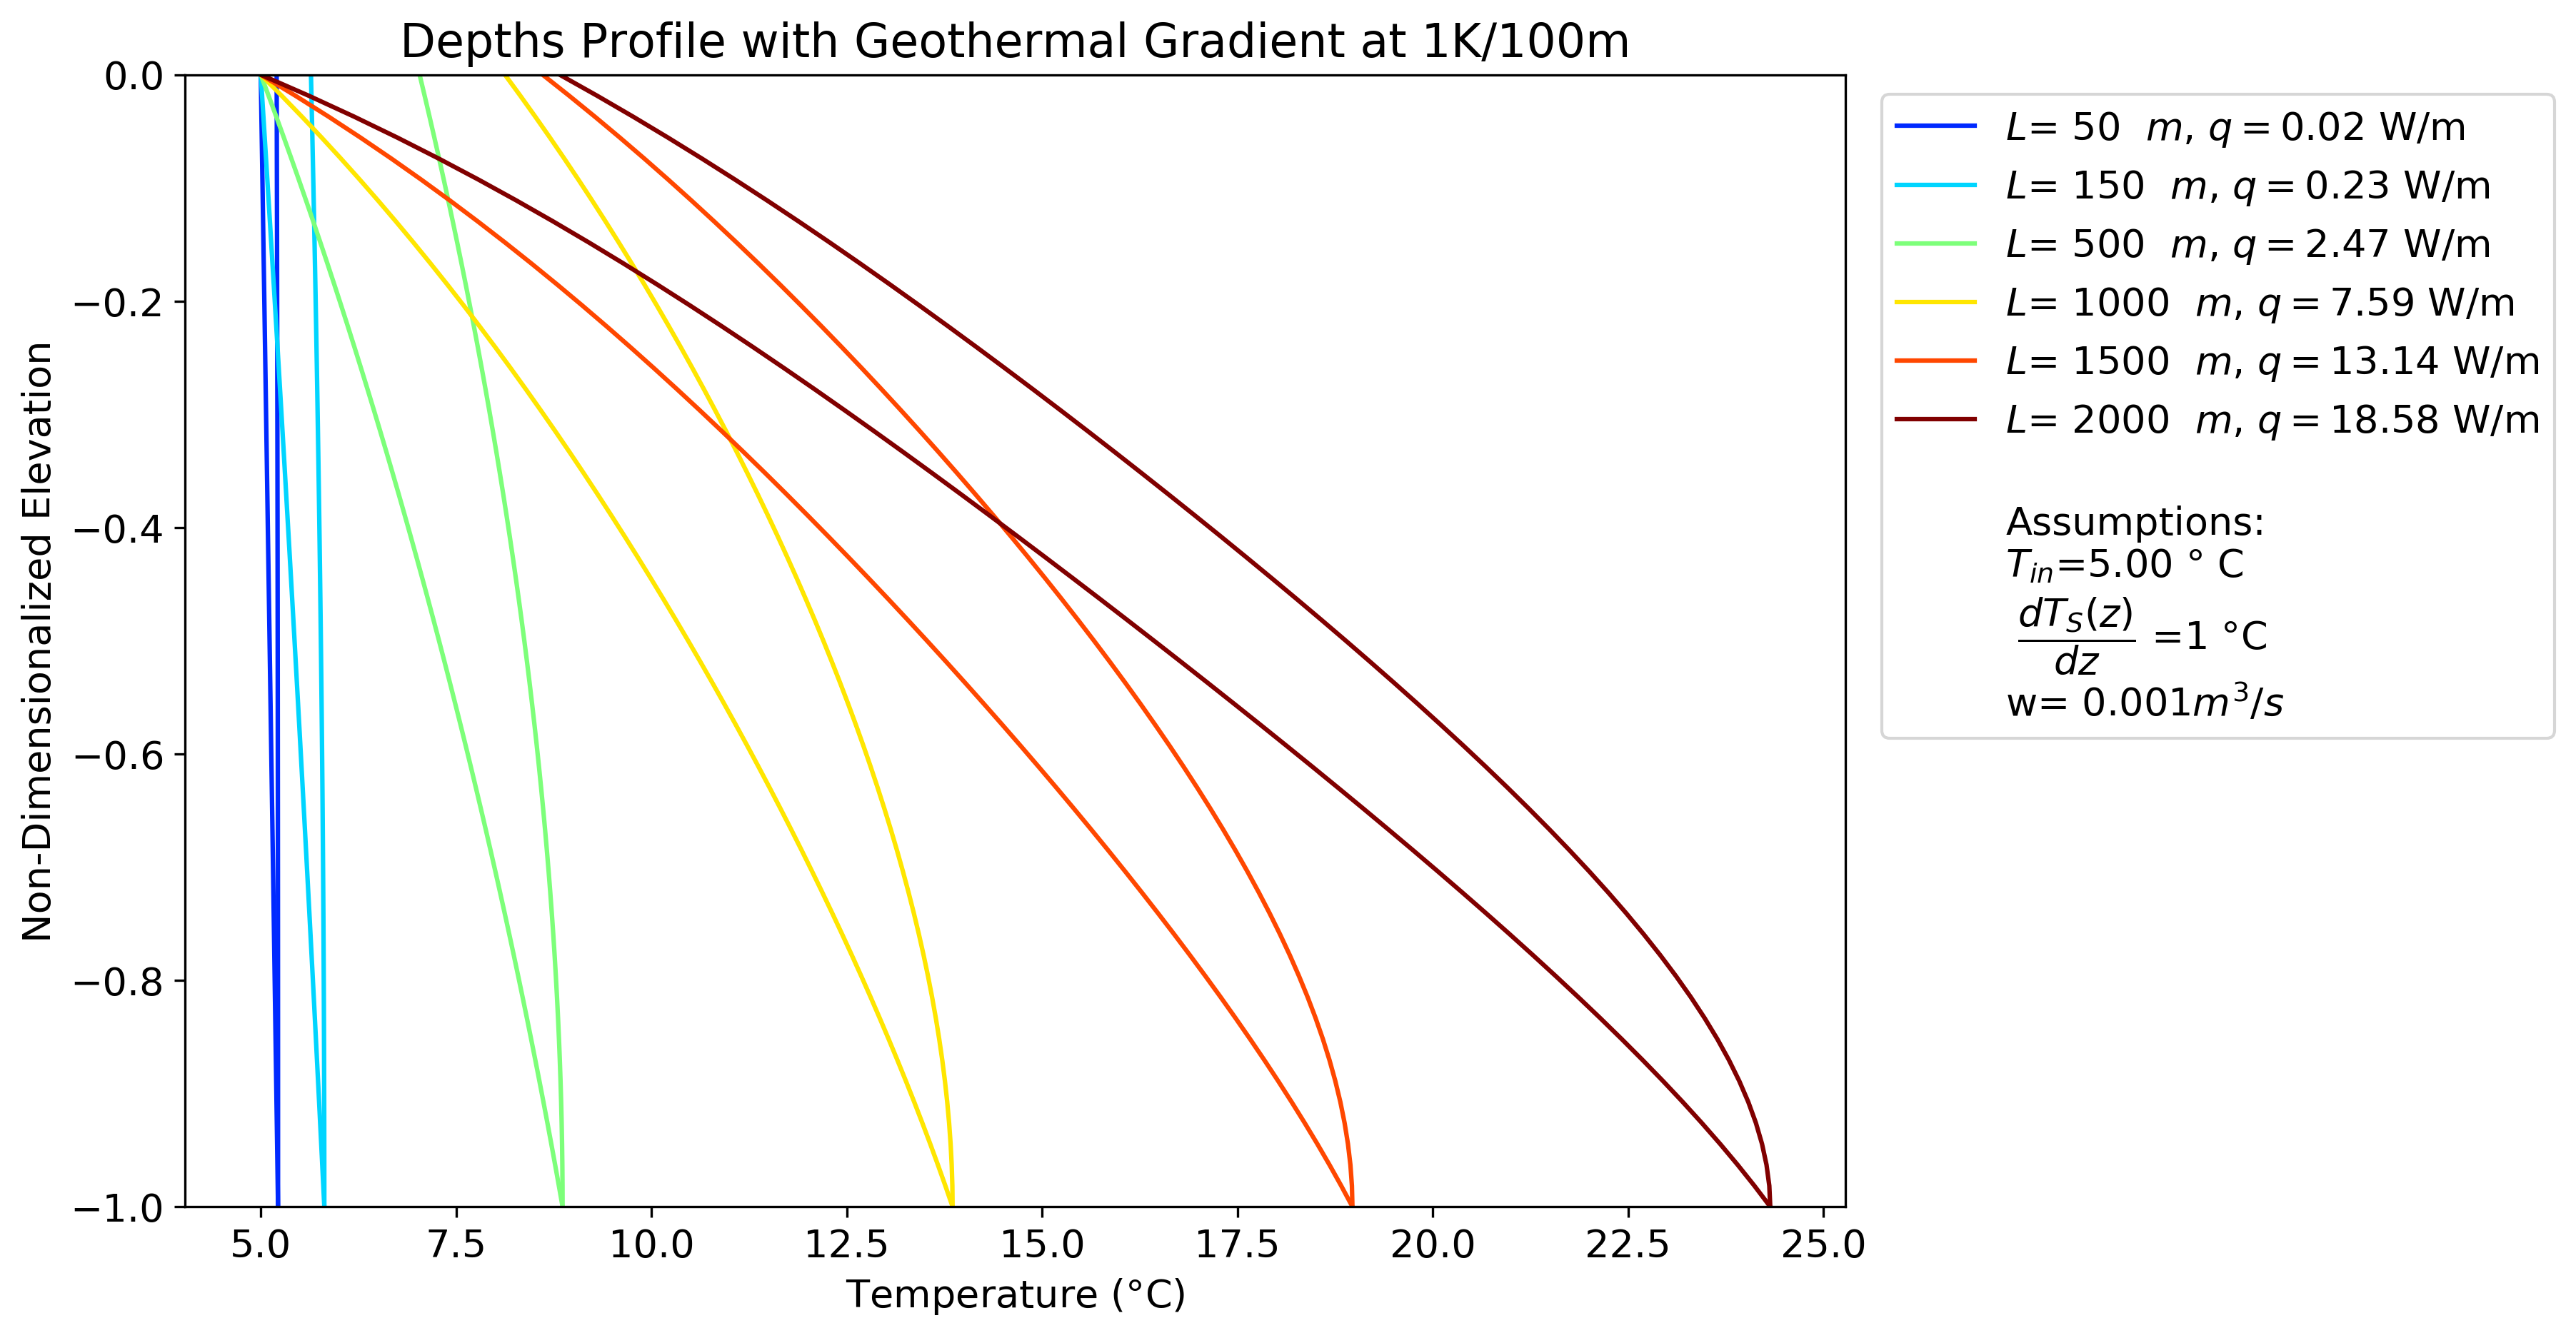
\includegraphics[width=0.75\textwidth]{depths_5_1k.png}
	        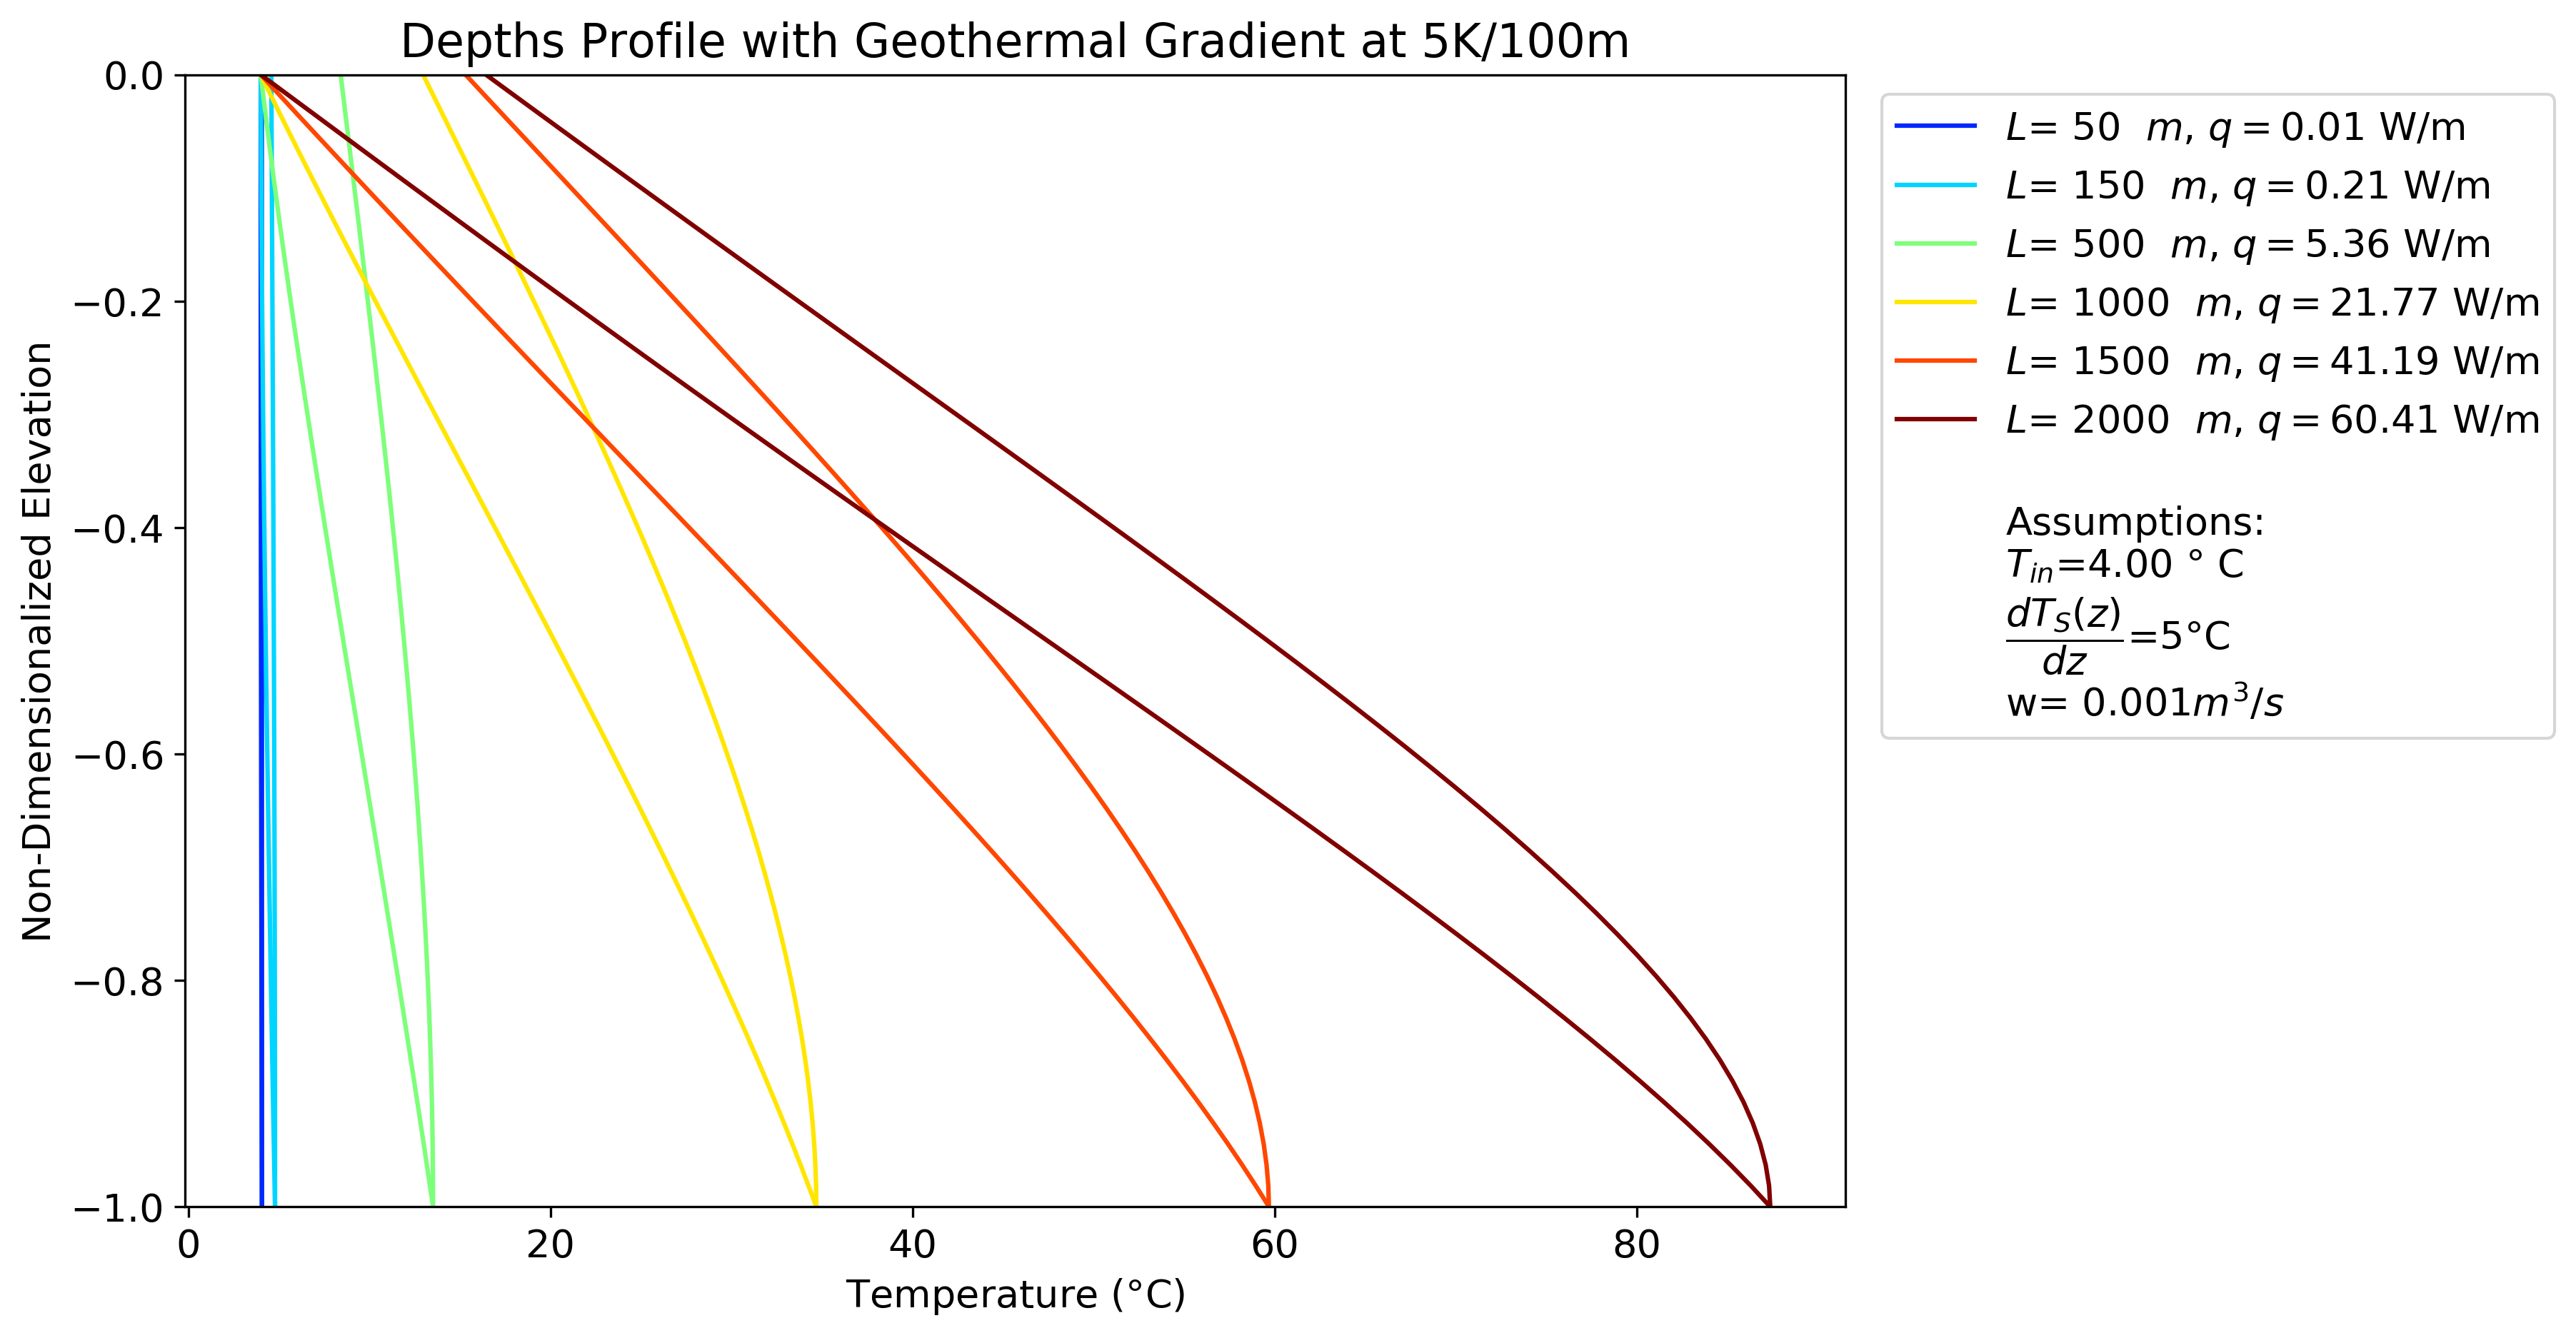
\includegraphics[width=0.75\textwidth]{depths_5_5k.png}
	        \caption{Vertical temperature distribution for the CBHE with original configuration for geothermal gradient of 1 Kelvin/100m(top) and 5 Kelvin/100m (bottom).}
	        \label{fig:GG}
	    \end{figure}
	    
		Similar to the discussion on the depths of CBHEs, deep CBHEs with large geothermal gradient produces the warmest temperatures at their bottom. Without proper insulation at the inner pipe and appropriate CBHE configuration, this thermal potential is difficult to recover for inadequately configured CBHE and flow rates. We're a geothermal gradient of 5 Kelvin per hundred meters, using the configuration already selected, the resulting temperature profile. As can be observed from Figure ~\ref{fig:5K}, the temperature out and the heat extraction rate are both much further improved for the deeper boreholes (L $\geq$ 1000m), while for shallower boreholes (L $\leq$ 500m), the benefit of insulating the inner pipe, increasing the pipe thickness or changing the flow rate did not create discernably visible differences. As the temperature at the outlet also exceeds 30 \degree C for the deeper boreholes, it is possible to use CBHEs for direct heating, but potentially with additional upper insulation where the injected water regenerates the upper part of the CBHE.
	    \begin{figure}[h!]
	        \centering
	        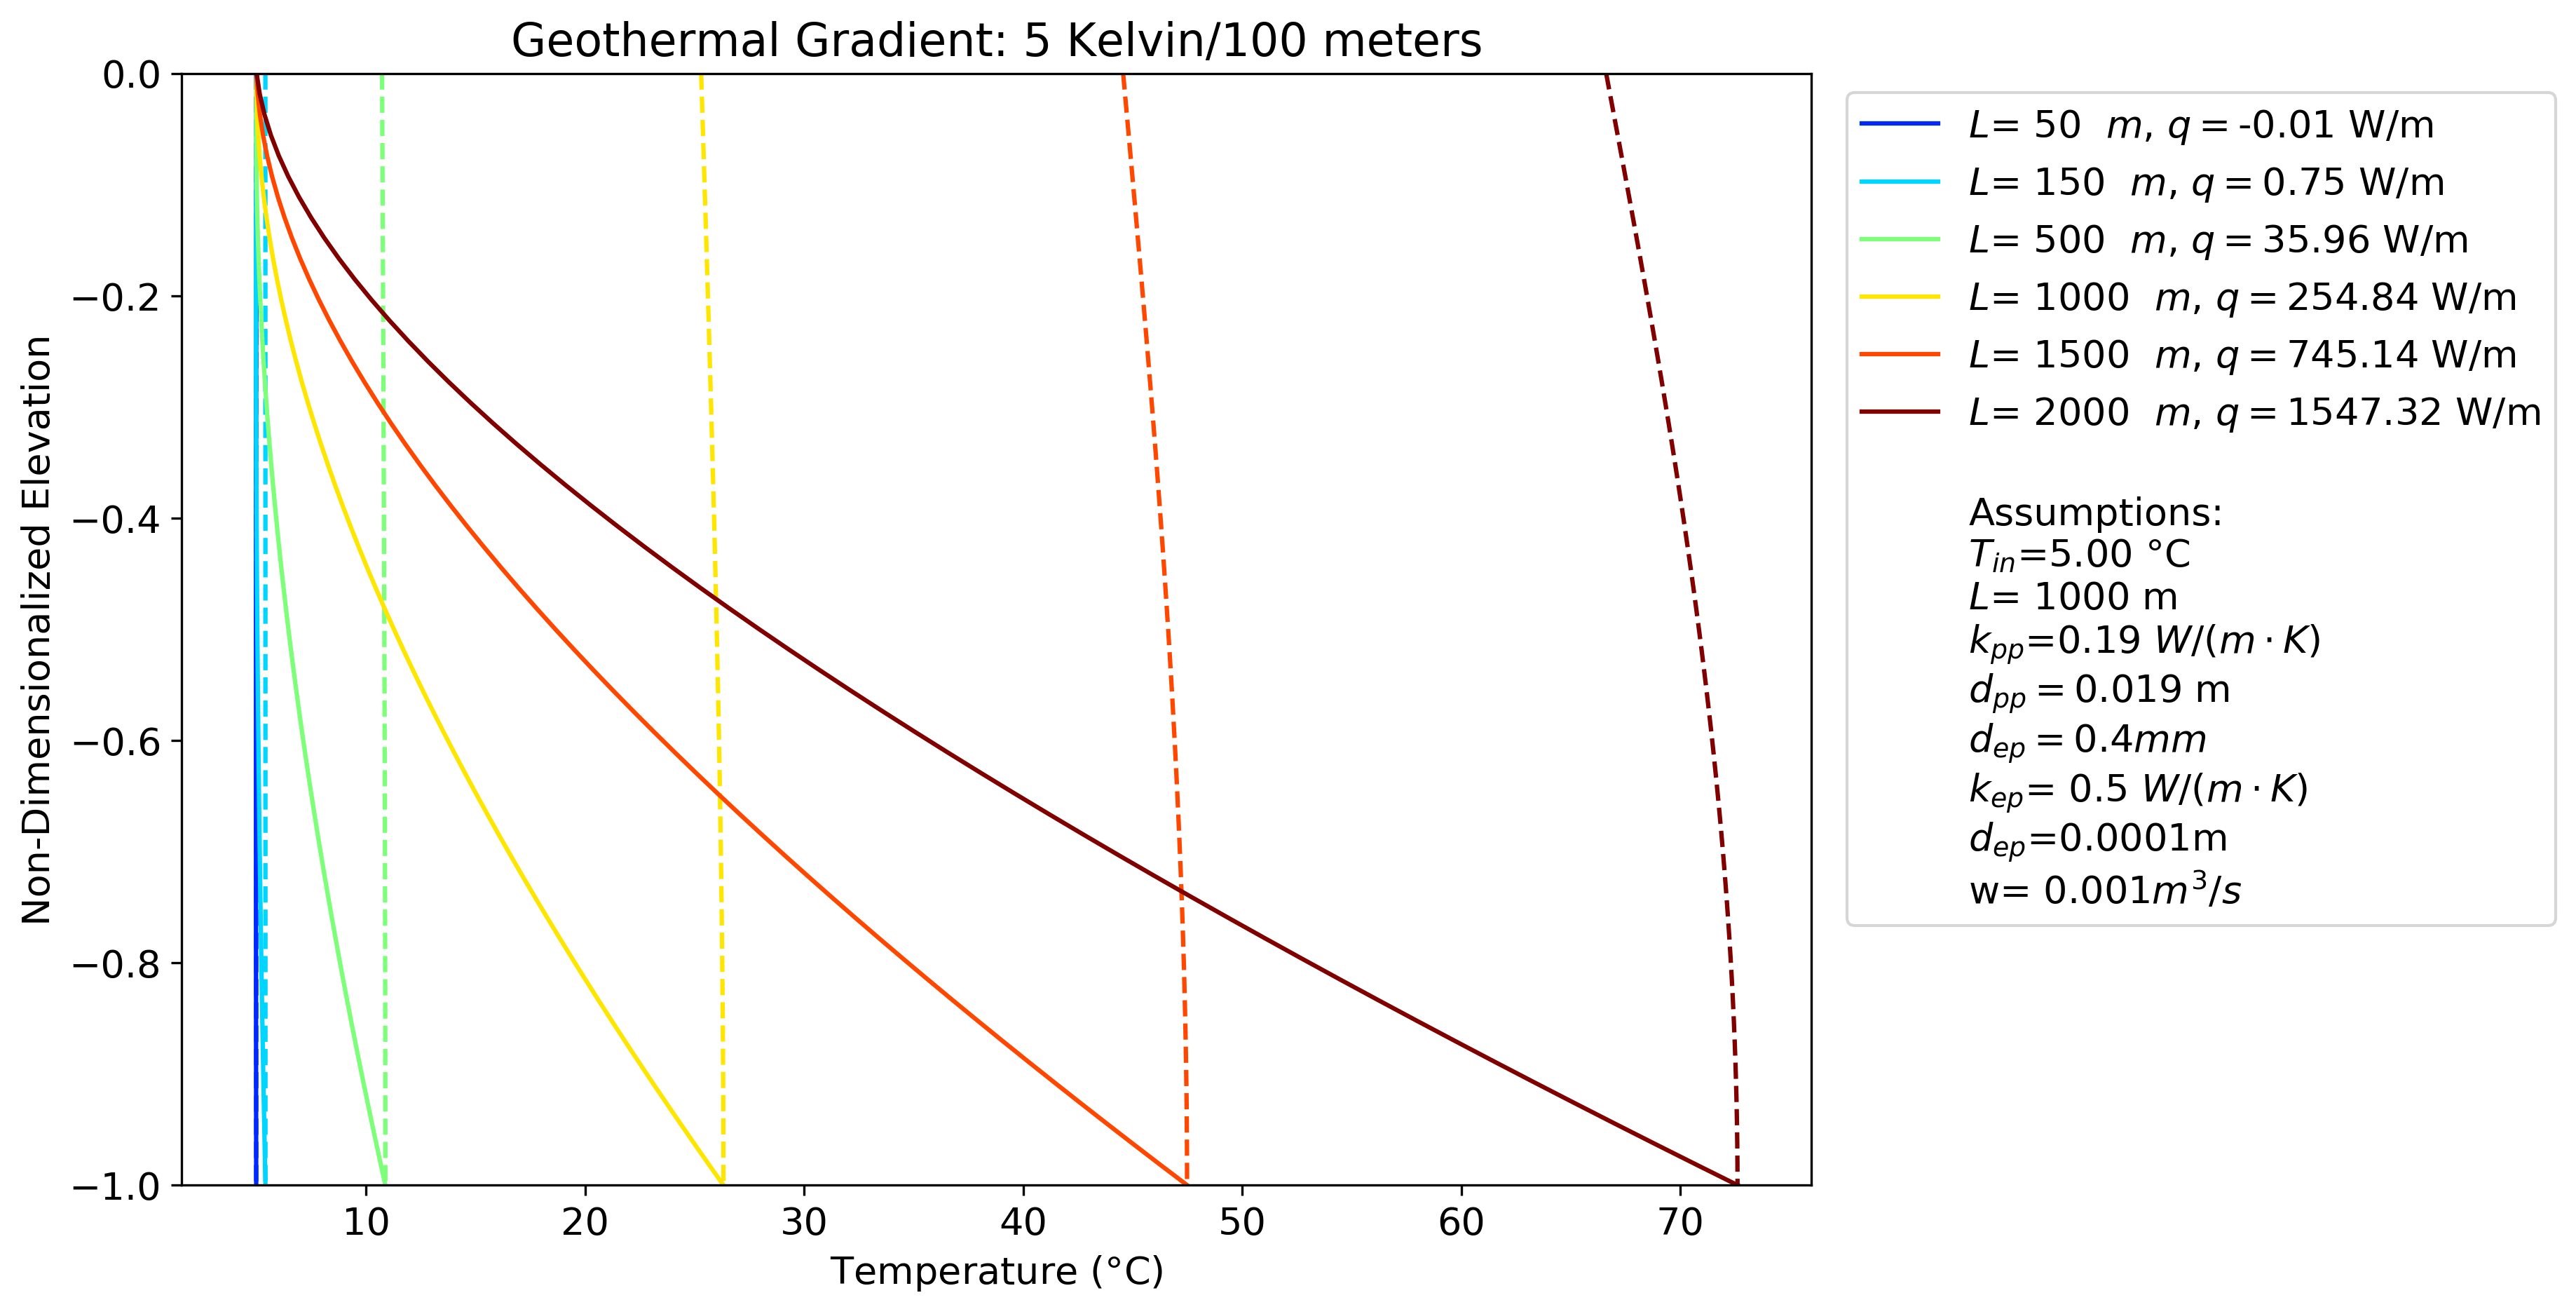
\includegraphics[width=0.75\textwidth]{depths_5_5k_Tin5_w3.png}
	        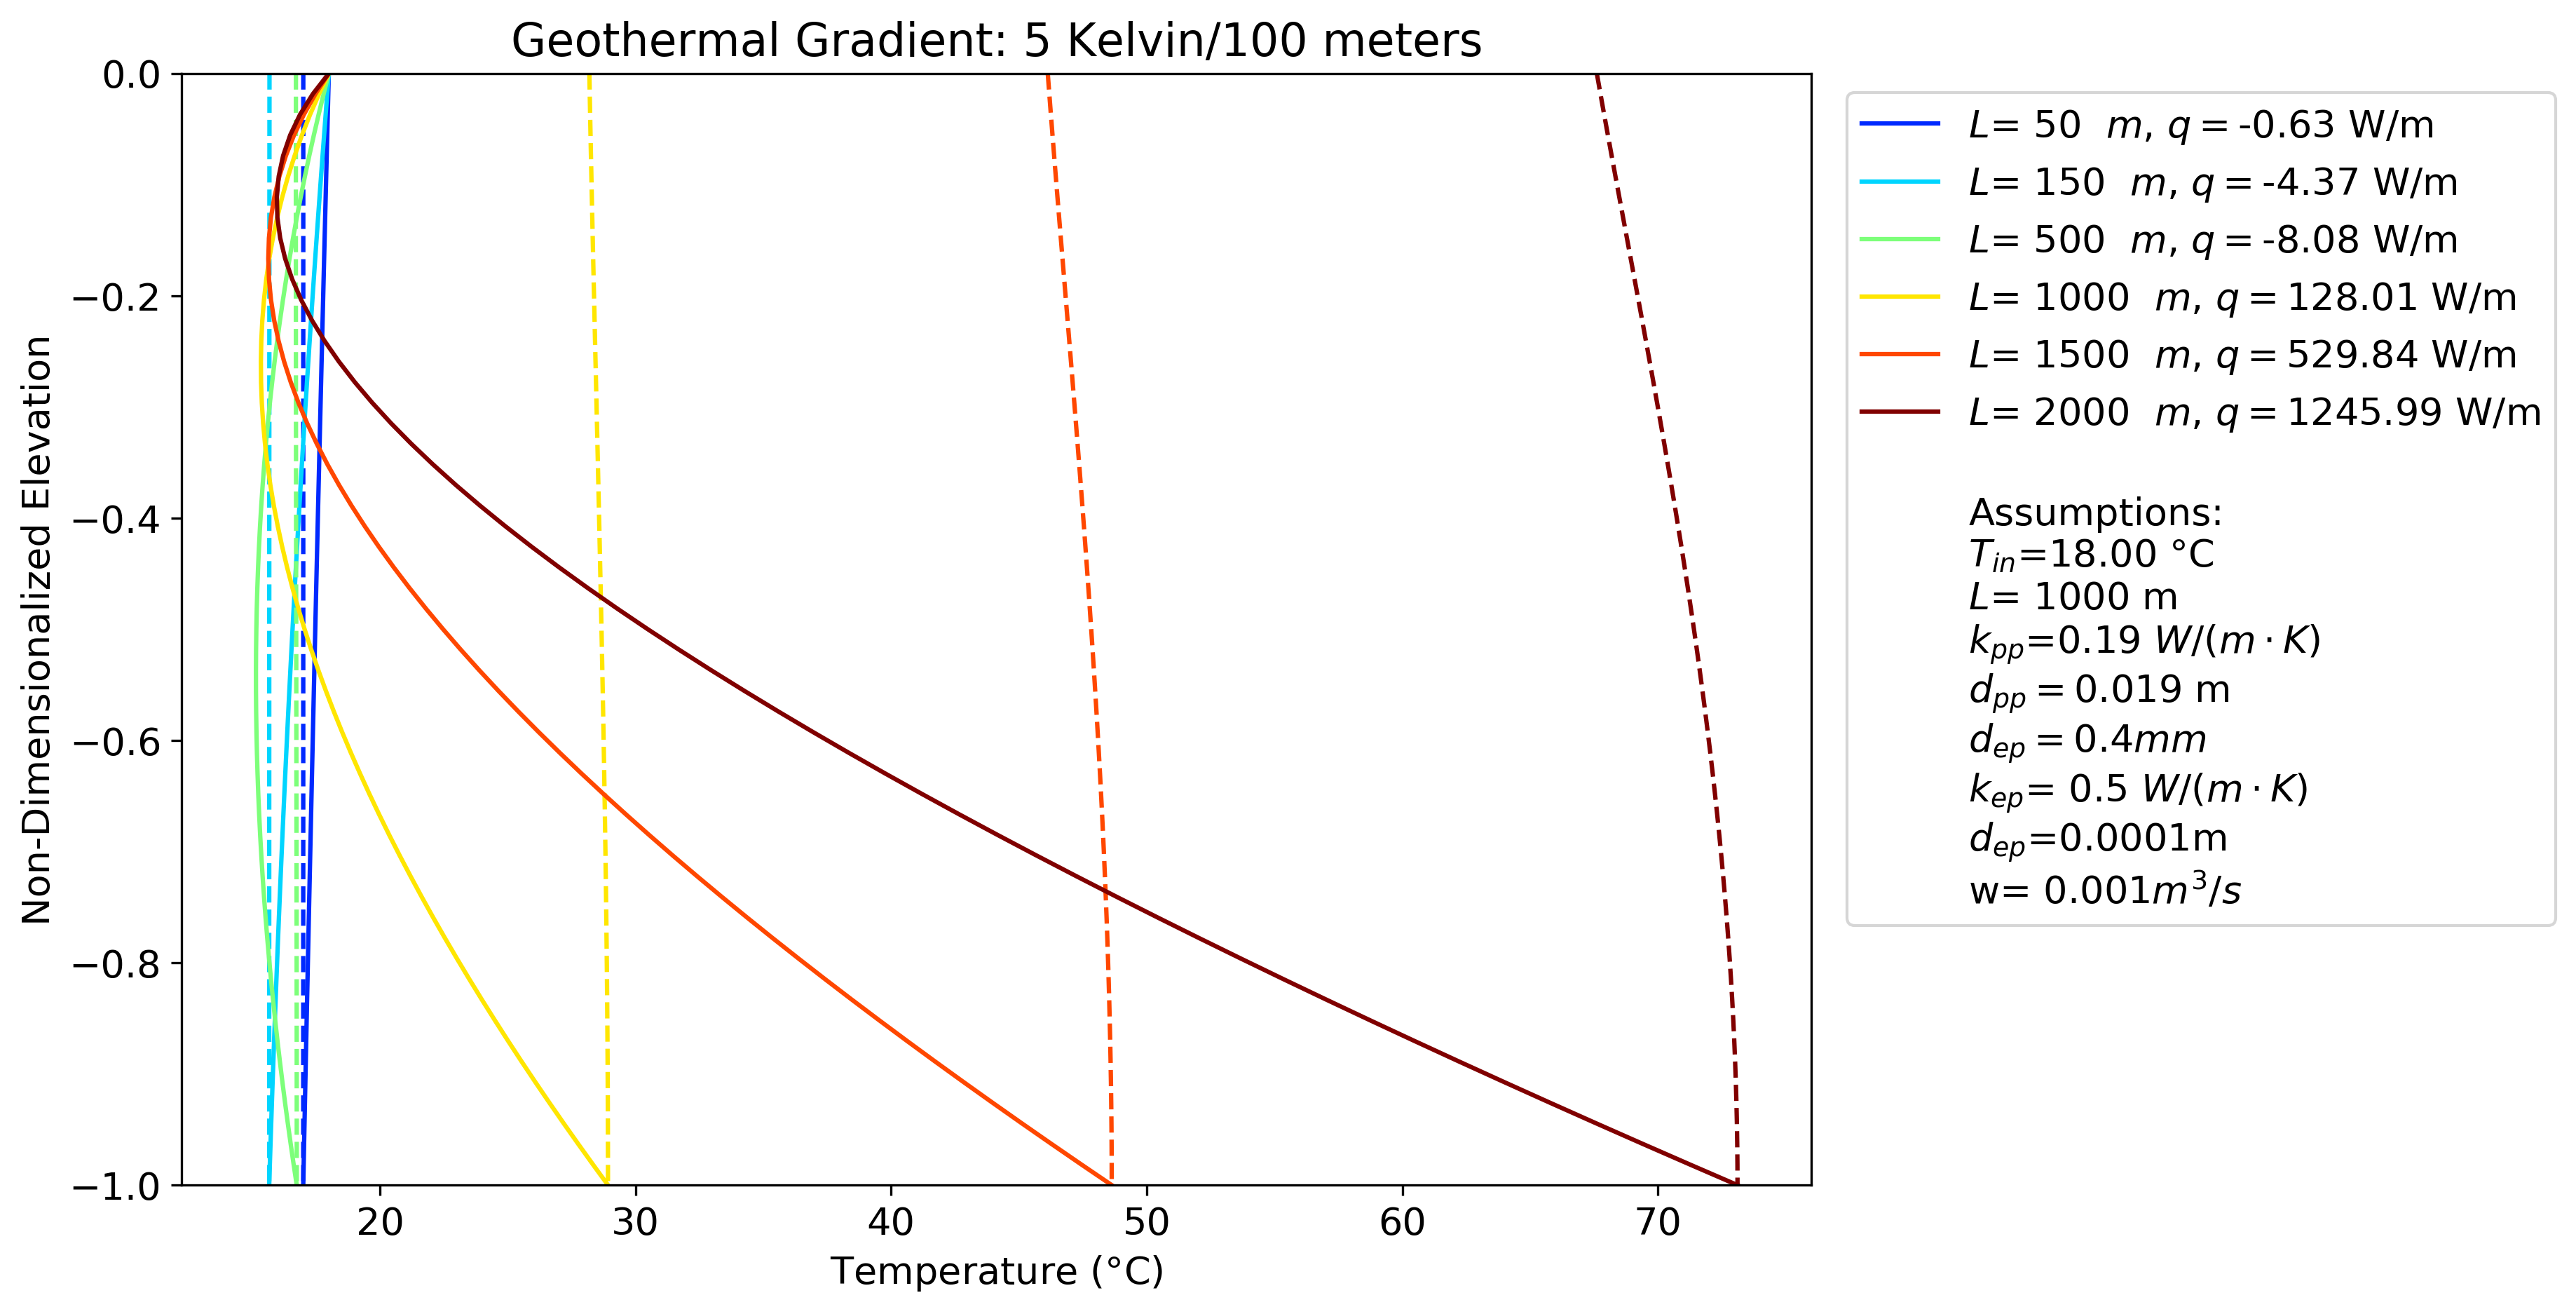
\includegraphics[width=0.75\textwidth]{depths_5_5k_Tin18_w3.png}
	        \caption{Vertical temperature distribution for the CBHE with original configuration for $T_{in} = 5\degree C$(top) and $T_{in} = 18\degree C$ (bottom) with a geothermal gradient of 5 Kelvin per hundred meters.}
	        \label{fig:5K}
	    \end{figure}
	    As can be observed from Figure~\ref{fig:5K}, the temperature out and the heat extraction rate are both much further improved for the deeper boreholes (L $\geq$ 1000m), while for shallower boreholes (L $\leq$ 500m), the benefit of insulating the inner pipe, increasing the pipe thickness or changing the flow rate did not create discernably visible differences. As the temperature at the outlet also exceeds 30 \degree C for the deeper boreholes, it is possible to use CBHEs for direct heating, but potentially with additional upper insulation where the injected water regenerates the upper part of the CBHE.    

		Similarly, for a geothermal gradient of 3 Kelvin per hundred meters, the temperature distribution inside the CBHE can be simulated at the 100th hour as Figure~\ref{fig:3K}. The resulting temperature distribution inside the borehole shows, in general, a smaller heat extraction rate when the injection temperature is 18 \degree C for boreholes that have a length L $\geq$ 1000m. The direct heating potential appears to only be available for boreholes that are deeper than 1500m according to Figure ~\ref{fig:3K} since the temperature out of L = 1000m drops to just 12.4 \degree C.
	        
	    % As can be observed from Figure~\ref{fig:5K}, the temperature out and the heat extraction rate are both much further improved for the deeper boreholes ($L\geq 1000m$), while for shallower boreholes ($L\leq 500m$), the benefit of insulating the inner pipe, increasing the pipe thickness or changing the flow rate was not obvious. As the temperature at the outlet also exceeds 30 $\degree C$ for the deeper boreholes, it is possible that CBHEs can be used for direct heating, but potentially with an additional upper insulation where the injected water regenerates the upper part of the CBHE.
	    
	    % Similarly for a geothermal gradient of 3 Kelvin per hundred meters, the temperature distribution inside the CBHE can be simulated at the 100th hour as Figure~\ref{fig:3K}. The resulting temperature distribution inside the borehole shows a in general a smaller heat extraction rate when the injection temperature is 18 $\degree C$ and can be observed for boreholes that has a length $L\geq 1000m$. The direct heating potential appears to only be available for boreholes that are deeper deeper than $1500 m$ according to Figure~\ref{fig:3K}, since the temperature out of $L=1000m$ drops to only 12.4 $\degree C$. 
	        
	    \begin{figure}[h!]
	        \centering
	        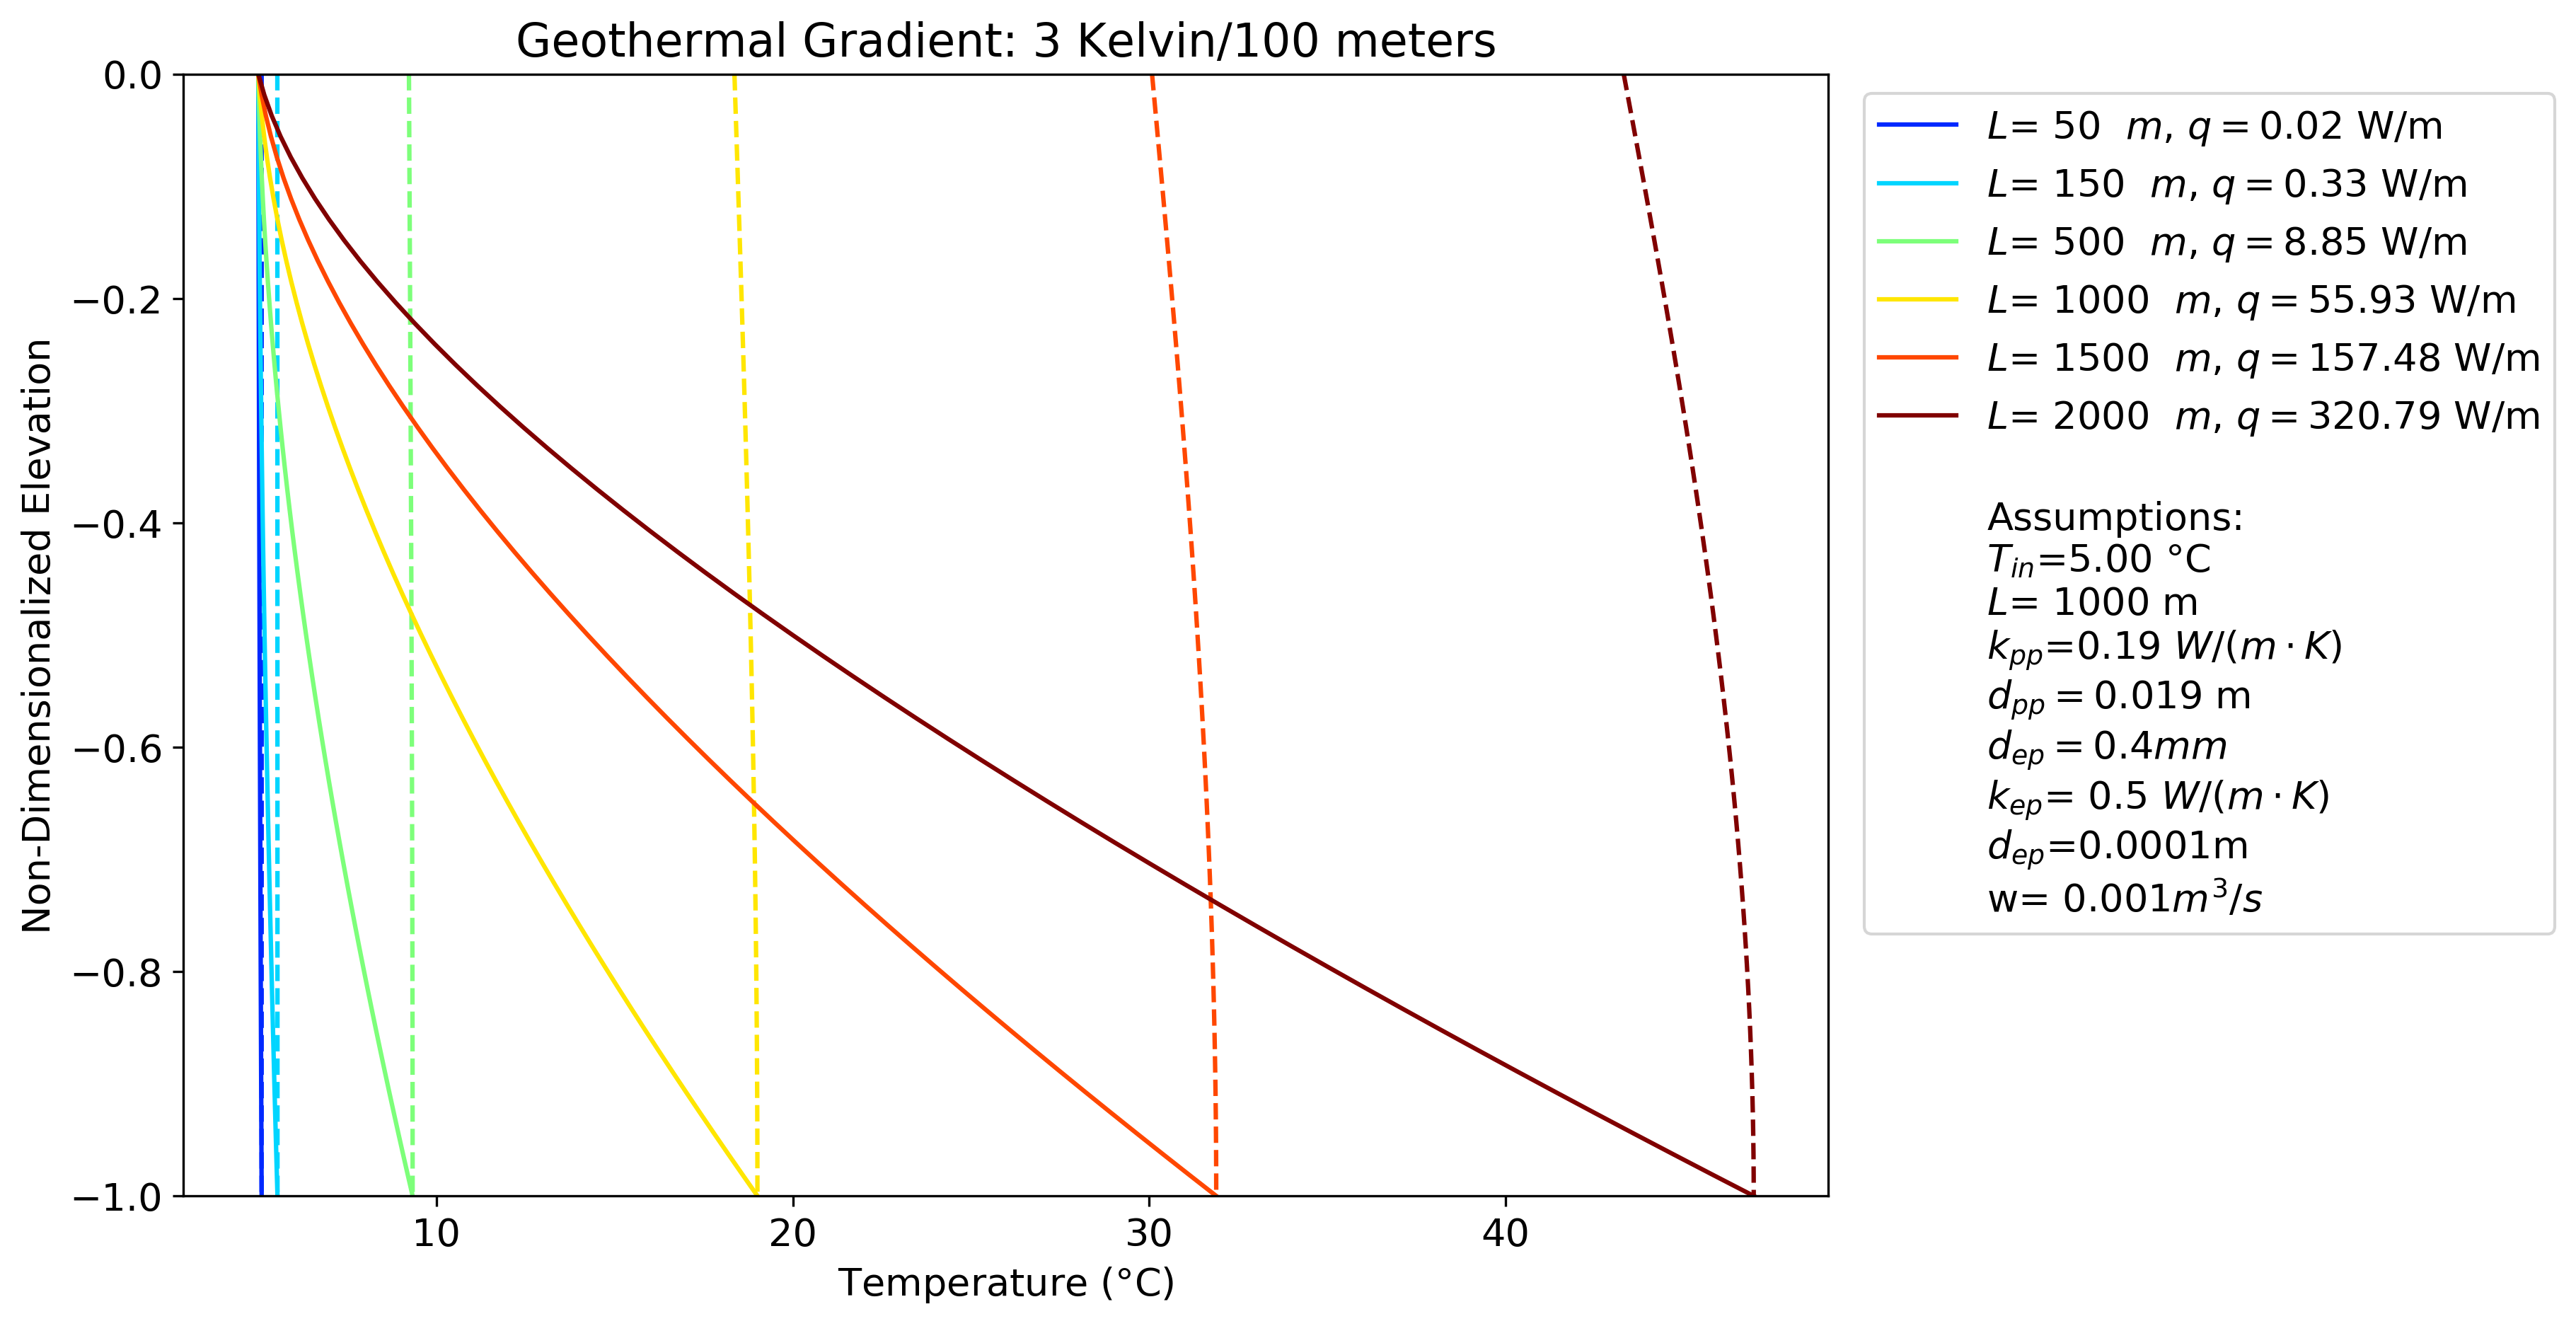
\includegraphics[width=0.75\textwidth]{depths_5_3k_Tin5_w3.png}
	        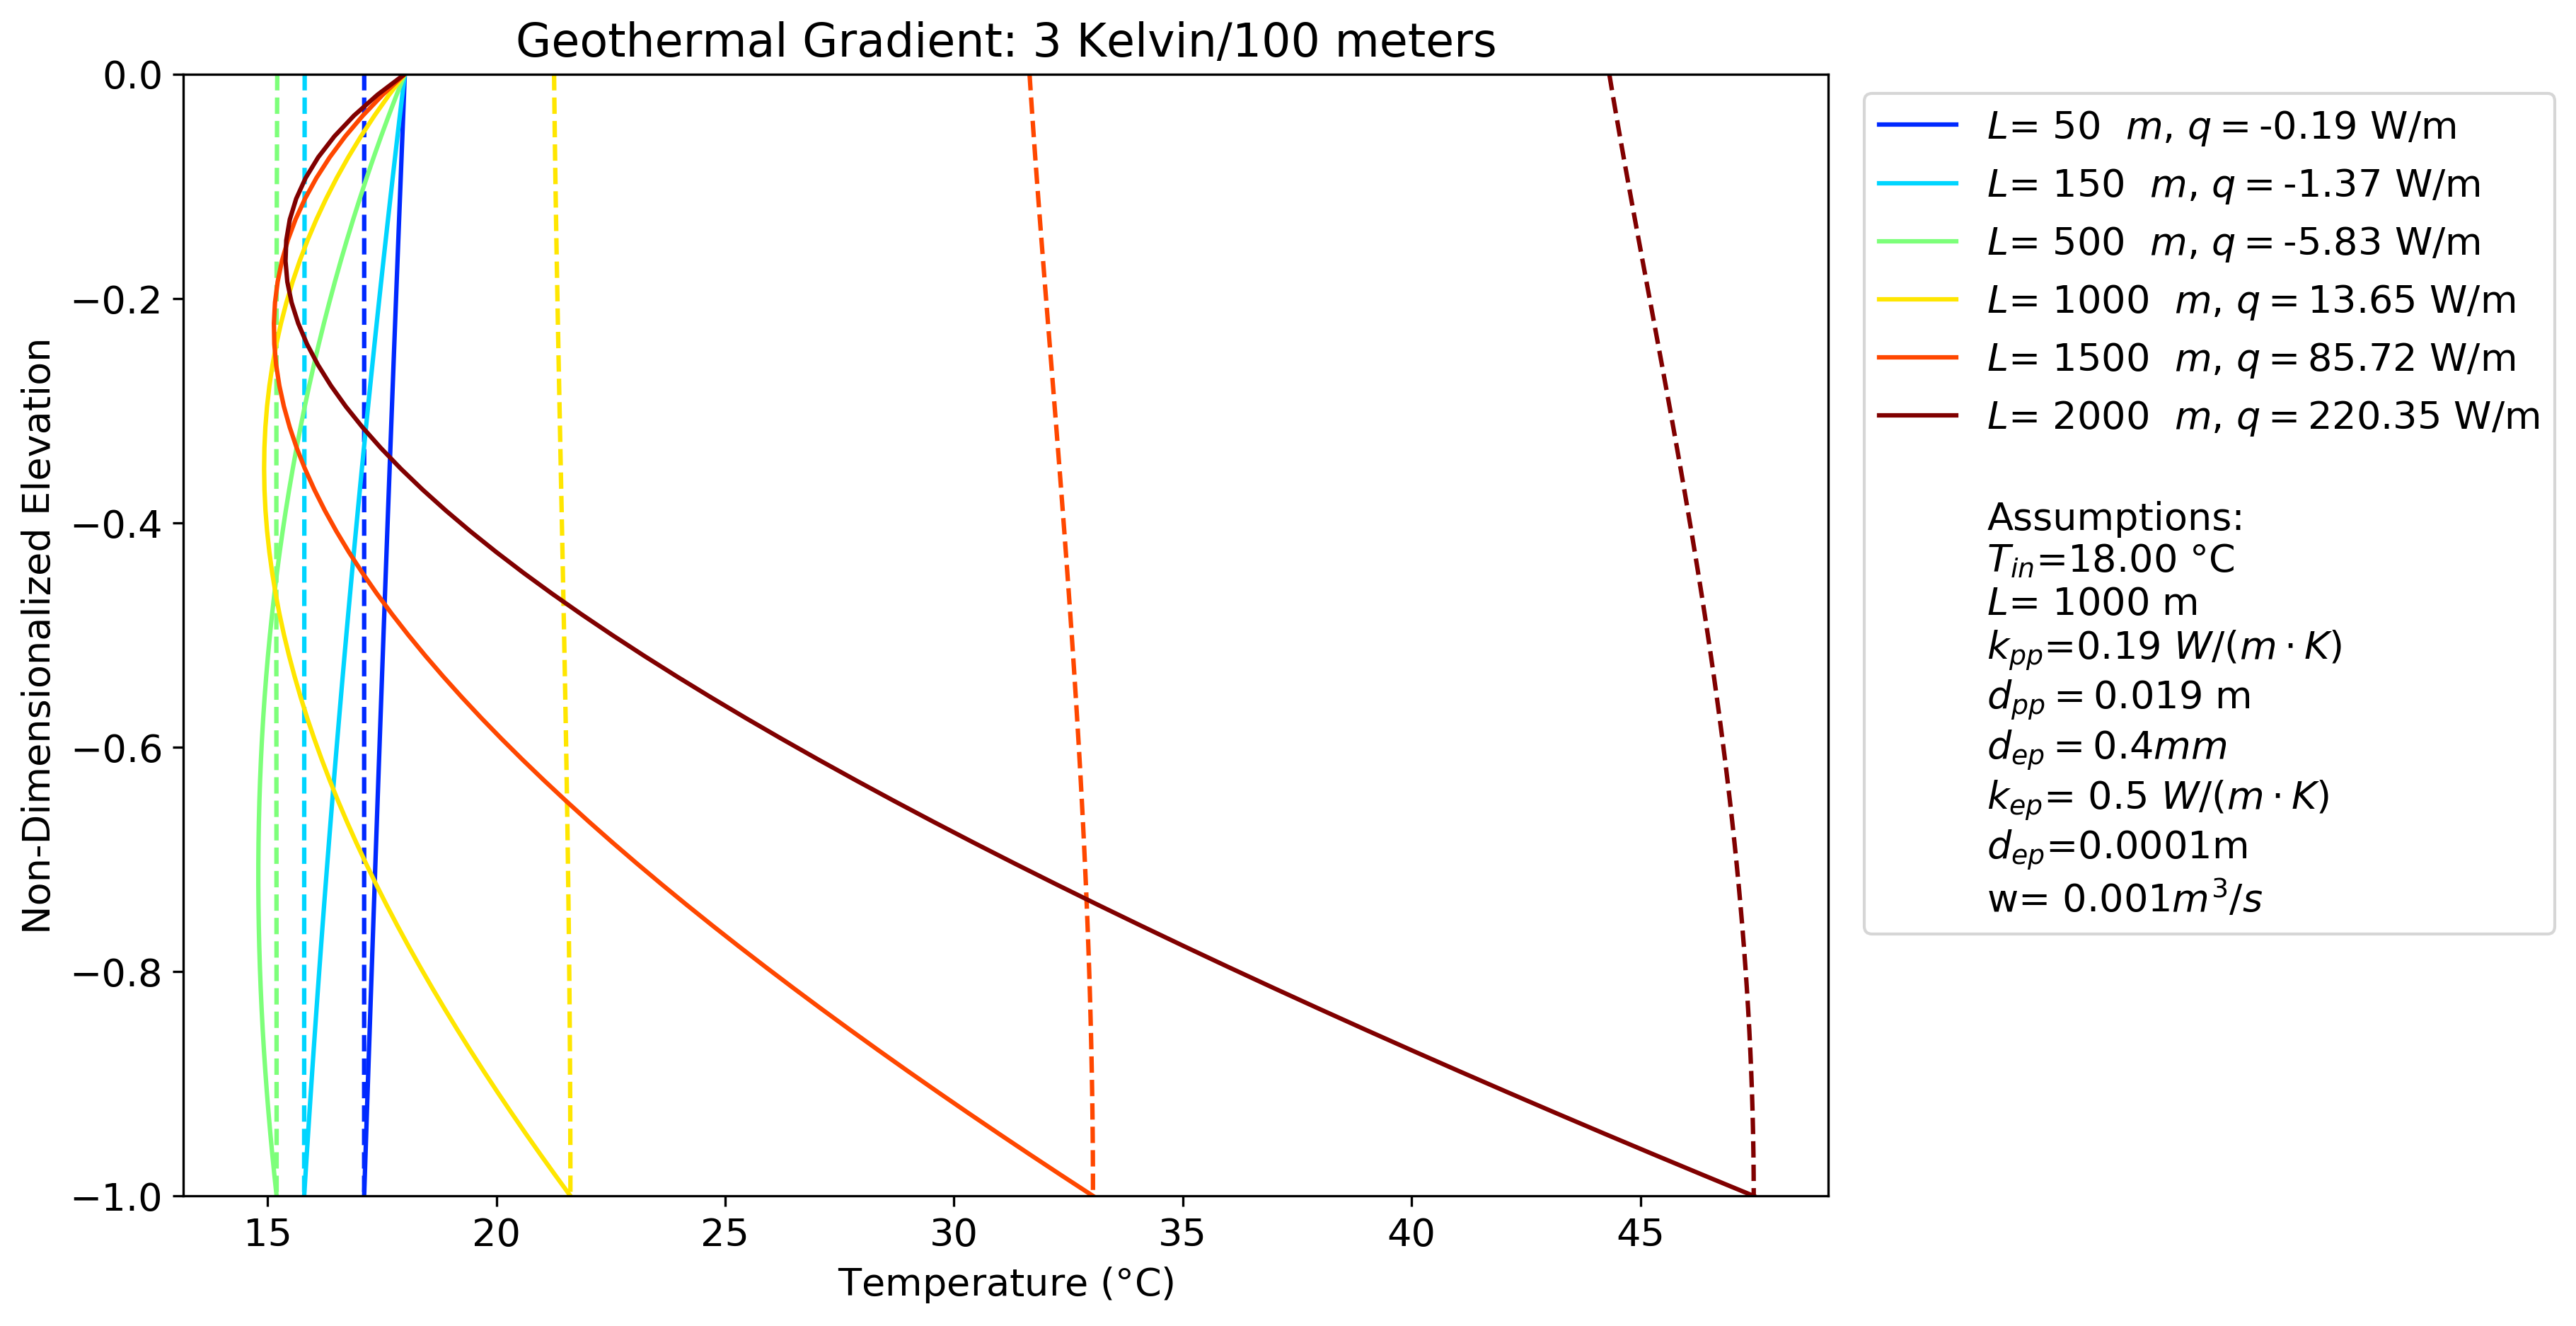
\includegraphics[width=0.75\textwidth]{depths_5_3k_Tin18_w3.png}
	        \caption{Vertical temperature distribution for the CBHE with original configuration for $T_{in} = 5\degree C$(top) and $T_{in} = 18\degree C$ (bottom) with a geothermal gradient of 3 Kelvin per hundred meters.}
	        \label{fig:3K}
	    \end{figure}
	    
		Also examining the lowest geothermal gradient of 1 Kelvin per hundred meters, the temperature distribution inside the CBHE can be simulated at the 100th hour as Figure~\ref{fig:1K}. Increasing the inlet temperature does not result in any improvement in heat extraction rate with any depth assigned. Injecting warmer water does appear to have effectively regenerated the borehole and can be seen as CBHEs being feasible for cooling when the geothermal gradient is smaller, or the well is shallower.
	        
	    \begin{figure}[h!]
	        \centering
	        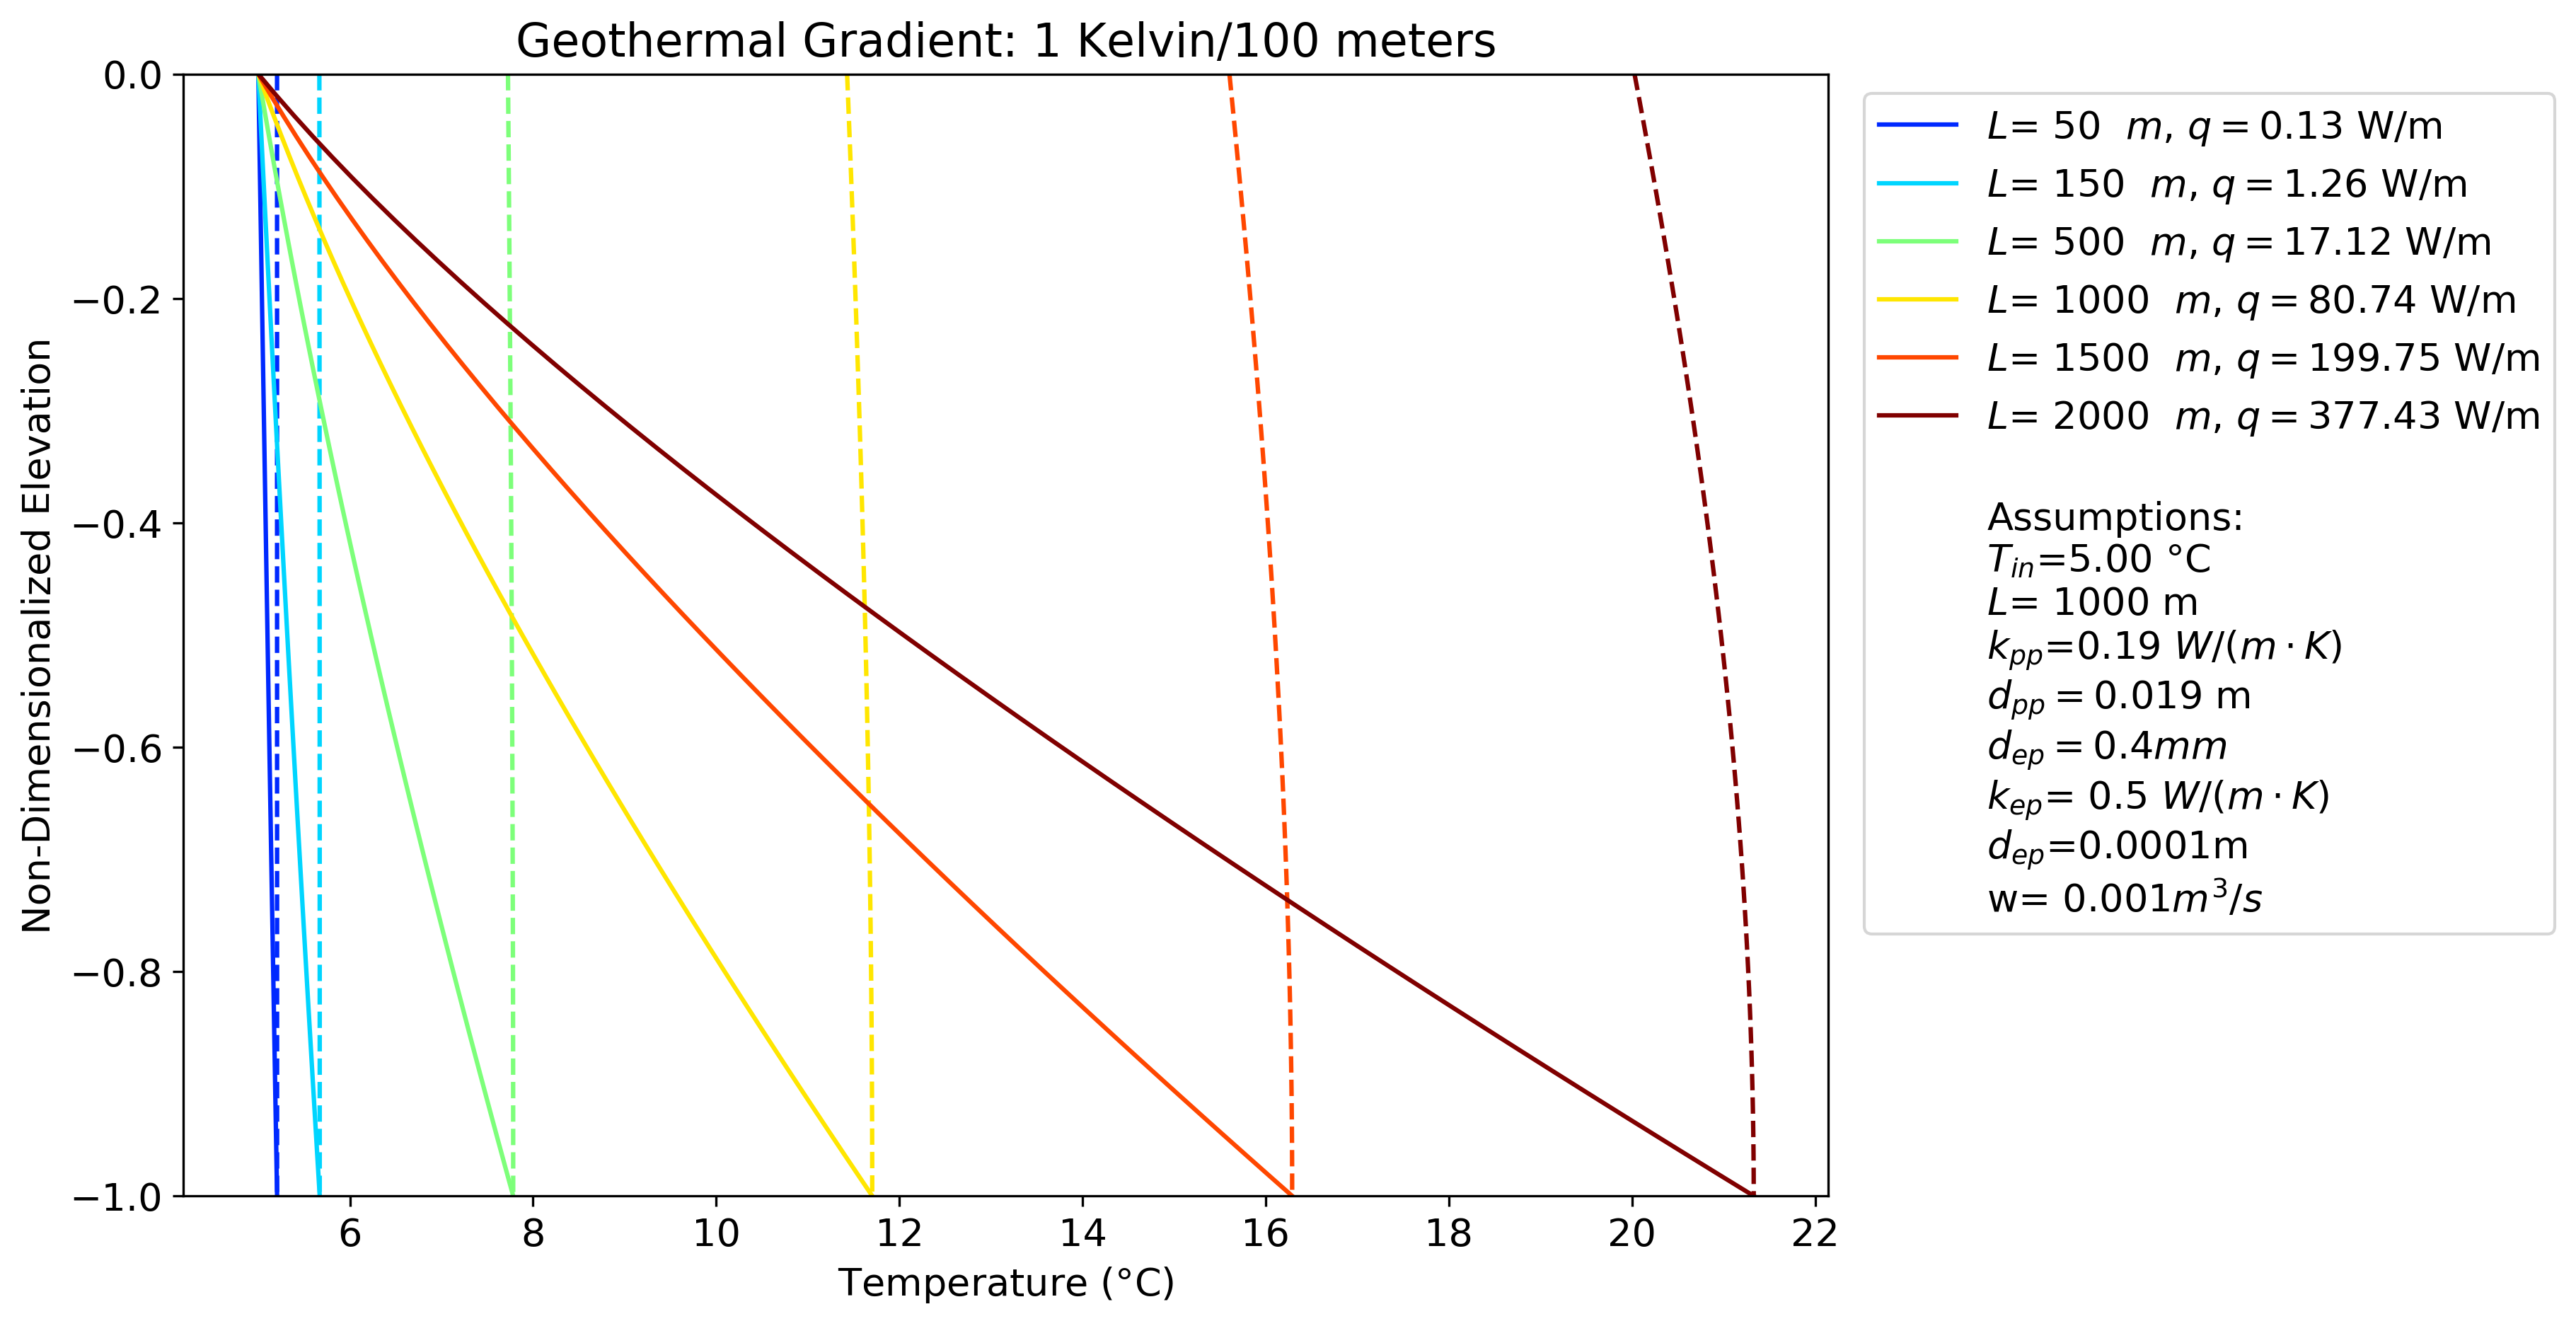
\includegraphics[width=0.75\textwidth]{depths_5_1k_Tin5_w3.png}
	        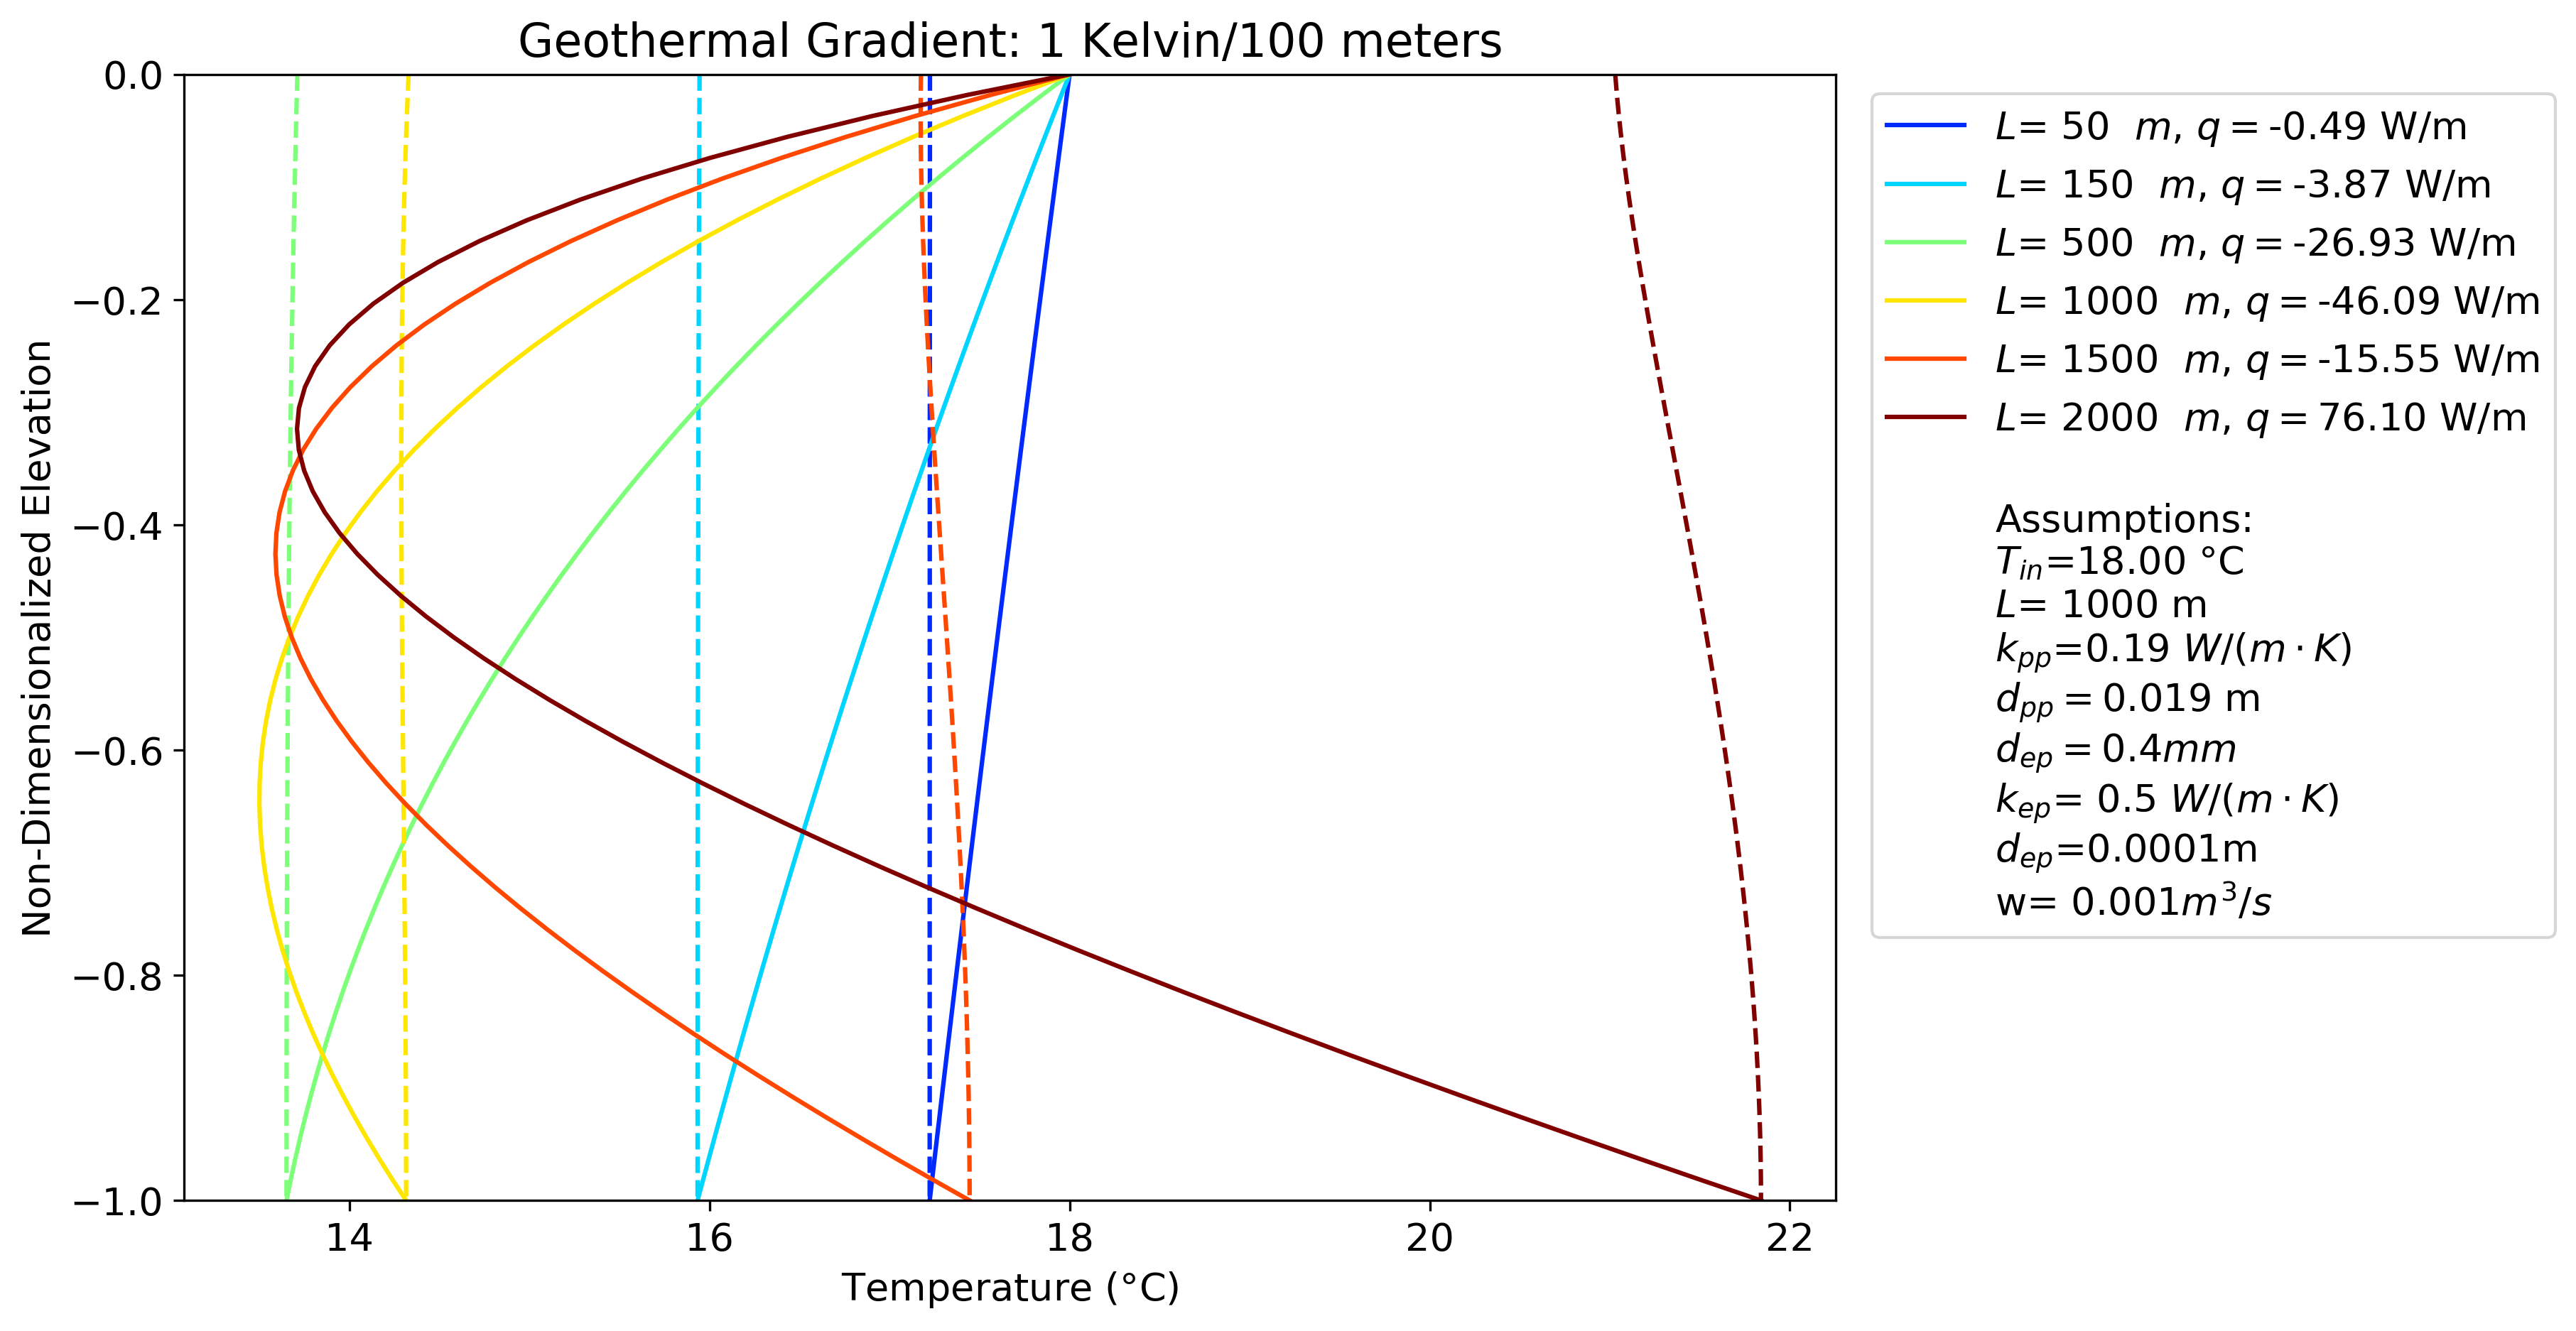
\includegraphics[width=0.75\textwidth]{depths_5_1k_Tin18_w3.png}
	        \caption{Vertical temperature distribution for the CBHE with original configuration for $T_{in} = 5\degree C$(top) and $T_{in} = 18\degree C$ (bottom) with a geothermal gradient of 1 Kelvin per hundred meters.}
	        \label{fig:1K}
	    \end{figure}
	   
	        \subsubsection{Soil thermal conductivity}
	        It is nearly impossible to determine the soil thermal conductivity before drilling and rigorous thermal response test (TRT), hence we only tested a specific range of possible thermal conductivity of soil, as shown in Figure~\ref{fig:ks}. In this scenario, the rest of the borehole parameters were held constant to test for the temperature increase along the flow path to determine the influence of the soil conductivity on the progressional heat transfer. The thermal conductivity of the ground, on the other hand, is set to vary between 2.5 to 3.5 $W/(m \cdot K)$, which led to the following results in Figure~\ref{fig:ks1000} for a 1000m-deep borehole.

	        % It is nearly impossible to determine the soil thermal conductivity before drilling and rigorous thermal response test (TRT), hence we only tested a specific range of possible thermal conductivity of soil, as shown in Figure~\ref{fig:ks}. In this scenario, the rest of the borehole parameters were hold constant to test for the temperature increase along the flow path to determine the influence of the soil conductivity on the progressional heat transfer. The thermal conductivity of the ground, on the other hand, is set to vary between 2.5 to 3.5 $W/(m\cdot K)$, which led to the following results in Figure~\ref{fig:ks1000} for a 1000m-deep borehole.
	        \begin{figure}[h!]
	            \centering
	            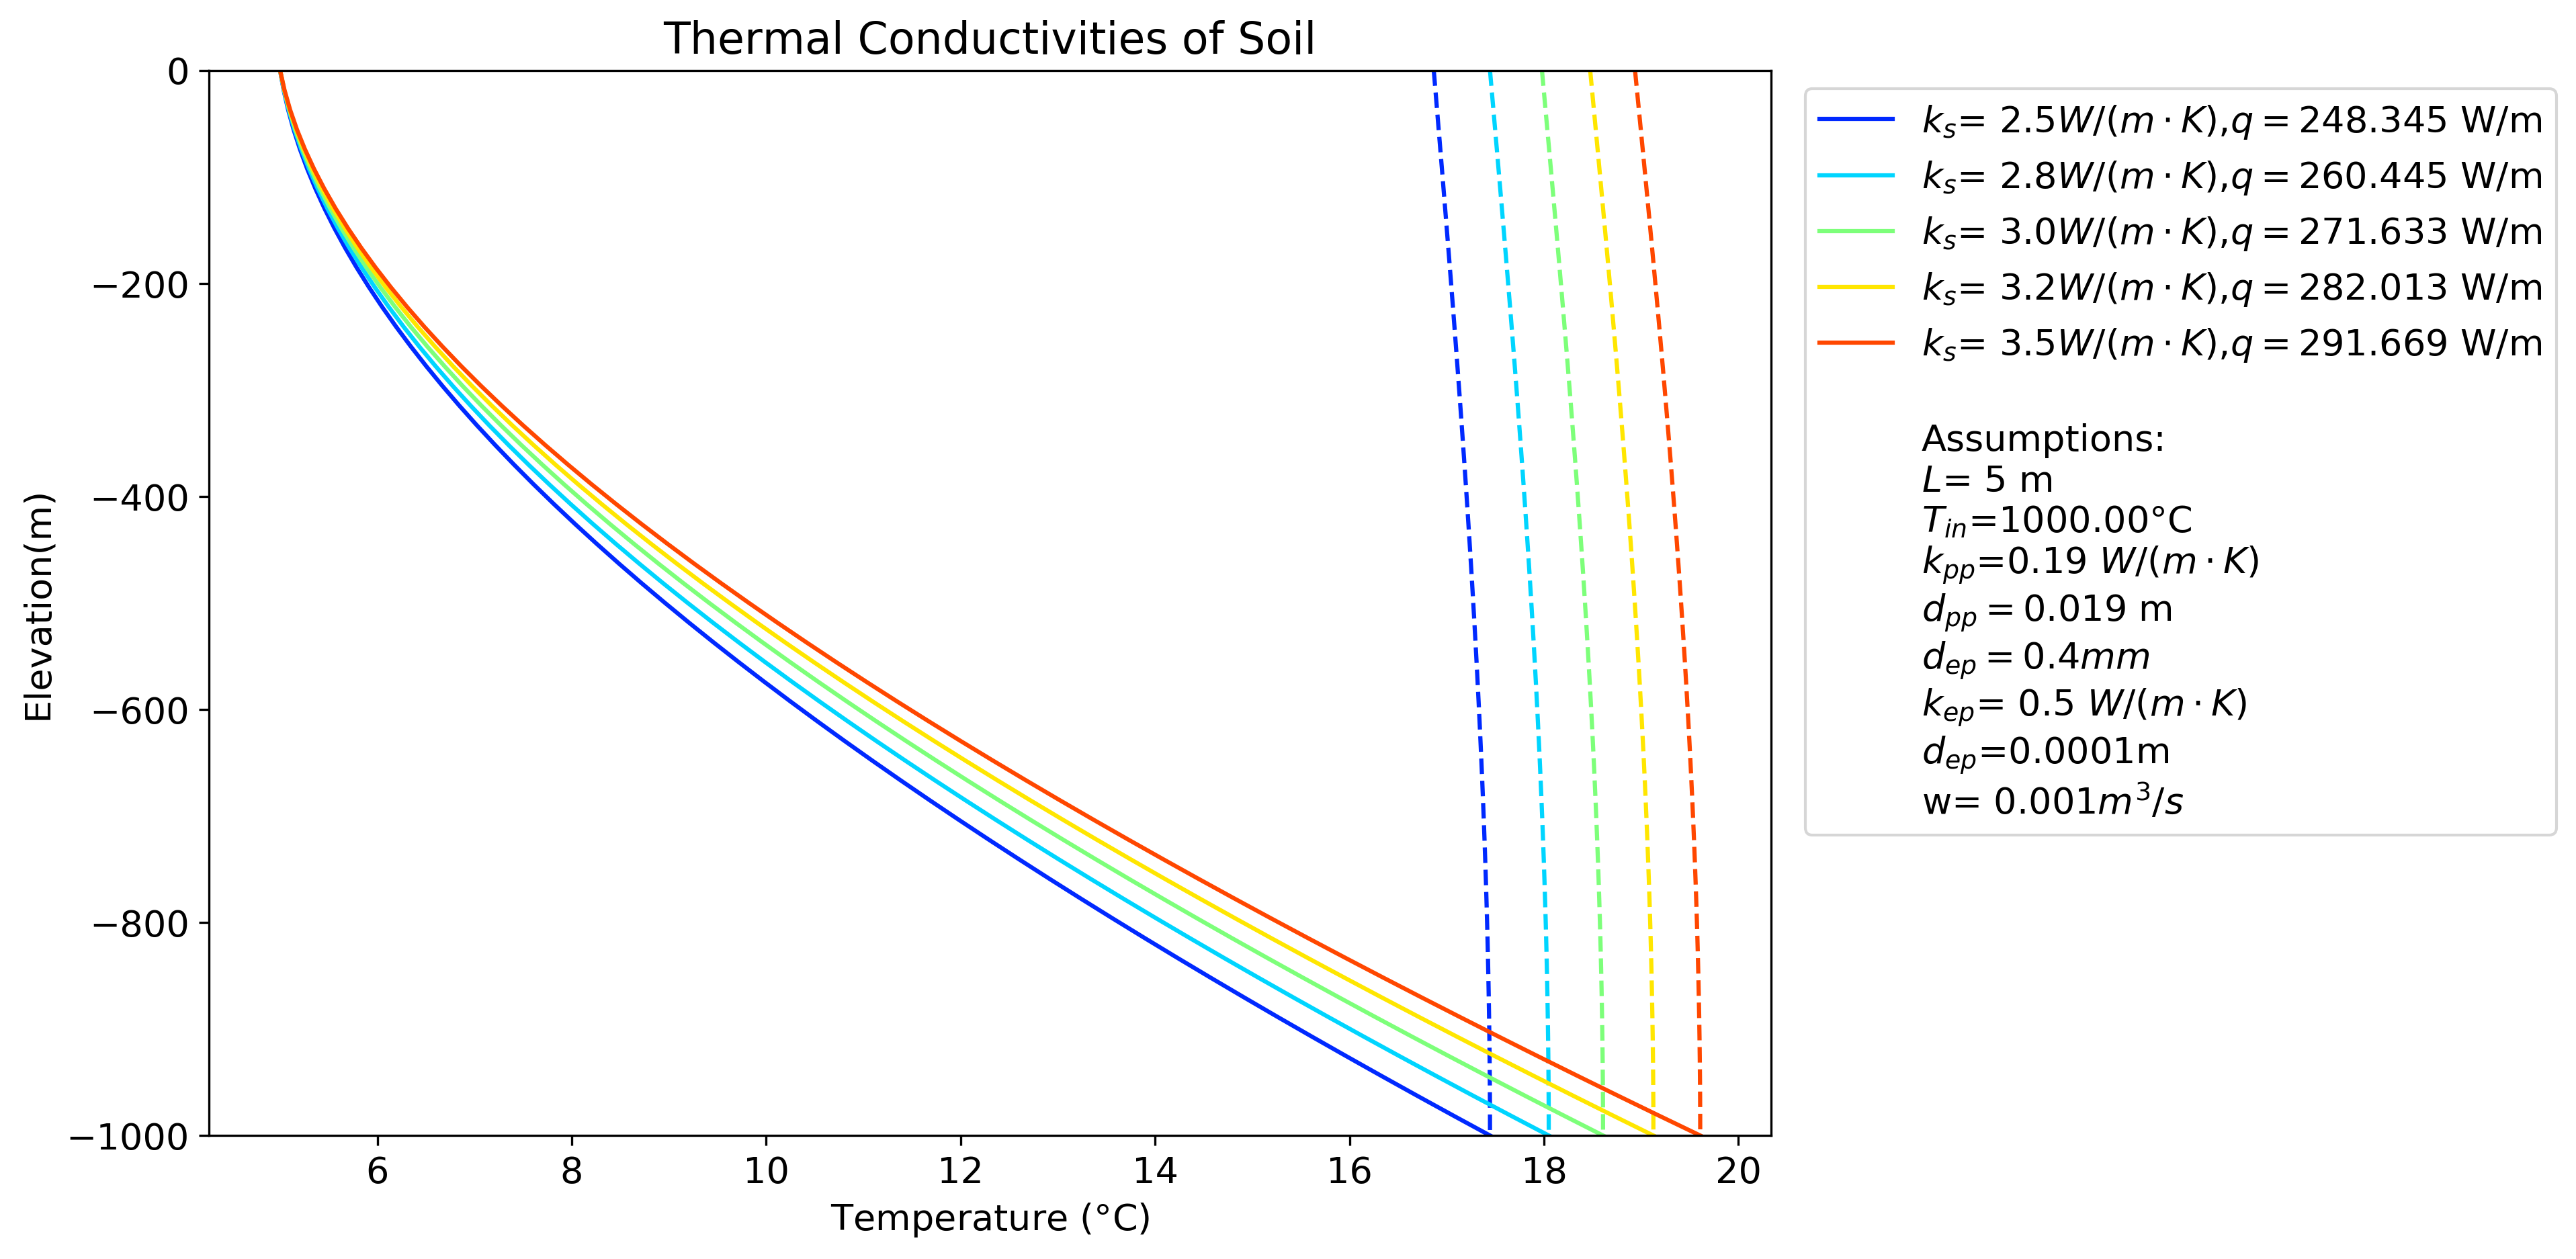
\includegraphics[width=0.75\textwidth]{ks_1000.png}
	            \caption{Influence of Soil Thermal Conductivity ($k_S$) on the thermal performance}\label{fig:ks}
	            \label{fig:ks1000}
	        \end{figure}
			The larger the soil conductivity, the more substantial amount of heat absorbed from the downward flow through the annulus, and maintains warmer through the upward inner pipe, as can be expected with consistent inner pipe thermal conductivities. This small temperature increase is slightly diminished from the temperature gradient between the downward and upward flow as is shown in Figure ~\ref{fig:ks1000}, where the outlet temperatures exhibit a smaller separation when compared to the temperature separation at the bottom of the borehole.
	    \subsubsection{Performance Implications}             
		The temperature variation along the distance travelled for a random water particle can also be tracked via the vertical temperature profile calculation as shown in Figure~\ref{fig:TempCOP} for a 1000m-deep CBHE with its key differences marked out in legends. The influence of our optimisation attempt was evident in the form of temperature at the outlet and heat extraction rate variation along the depth.  The temperature lift through the entire CBHE defines the overall performance cap through Carnot efficiency. We found varying both the flow rate and the thickness of the inner pipe may lead to a central pipe condition that is close to lossless along the outlet channel, while the thermal conductivity of the pipe does not change the resulting heating potential significant. This graph does not capture the added complexity when depth also becomes a variable for optimisation. A multivariate analysis that utilises either Monte Carlo methods or other statistical approaches could be beneficial to determine the improvement of proposed design over one another instead of the results shown here in Figure~\ref{fig:TempCOP}.
	        
		By changing the configuration and/or thermal properties of a CBHE, it is possible to either have the heat exchange along the downward (annulus) pathway increased, resulting in raised bottom of borehole temperature, as is with the case of varying the soil thermal conductivity between 2.5 and 3.5 $W/(m \cdot K)$, or changing the thickness of the borehole wall to 0.01 m. The latter also decreases the temperature along the upward (inner pipe) pathway, which can be made possible by assigning an ideal thermal conductivity of an inner pipe at a thermal conductivity of $k_{pp}$ = 0.007 $W/(m \cdot K)$ which is difficult to implement in real projects as it was the thermal conductivity of vacuum-insulated steel pipes. As was pointed out in the discussion for varying the flow rate, however, an alternative to achieve maximised COP with a minimised geothermal depletion by using a significantly increased flow rate to produce turbulence flow inside the inner pipe to harvest the increased temperature at the bottom of the CBHE. The resulting COP from the CBHE will likely not only be a function of the temperature of water at the outlet, the flow rate, but also the amount of pumping power (operational cost) that went into ensuring the functioning of the overall system, which goes beyond the scope of this current paper.
	        \begin{figure}
	            \centering
	            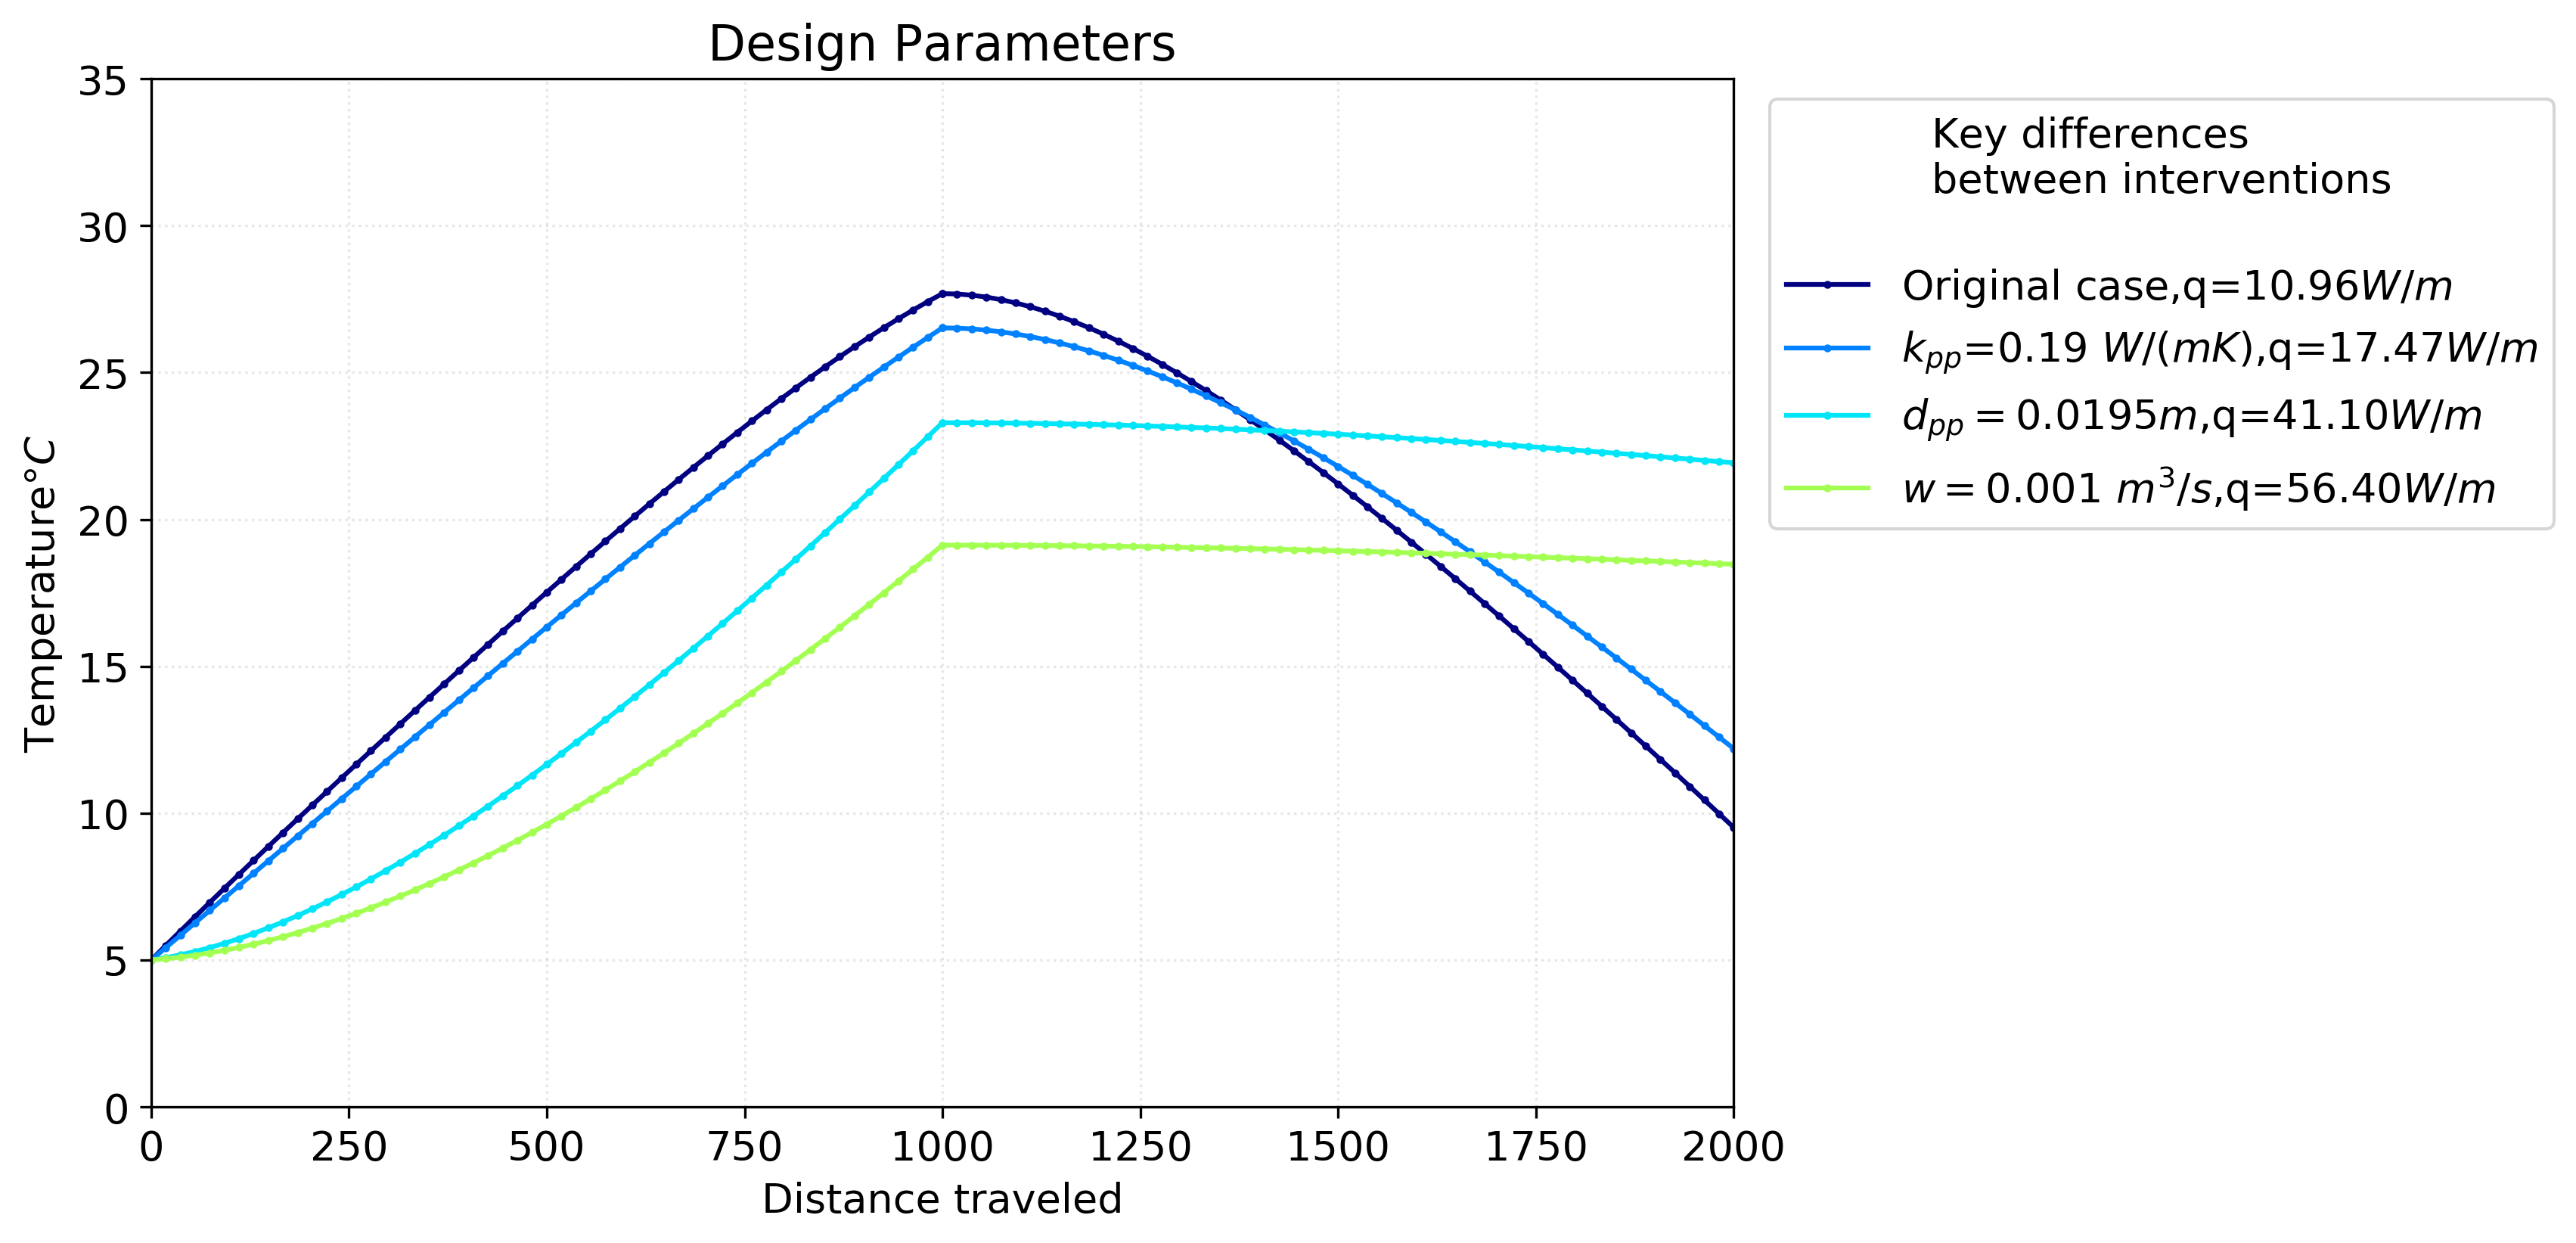
\includegraphics[width=0.75\textwidth]{DesignVars.png}
	            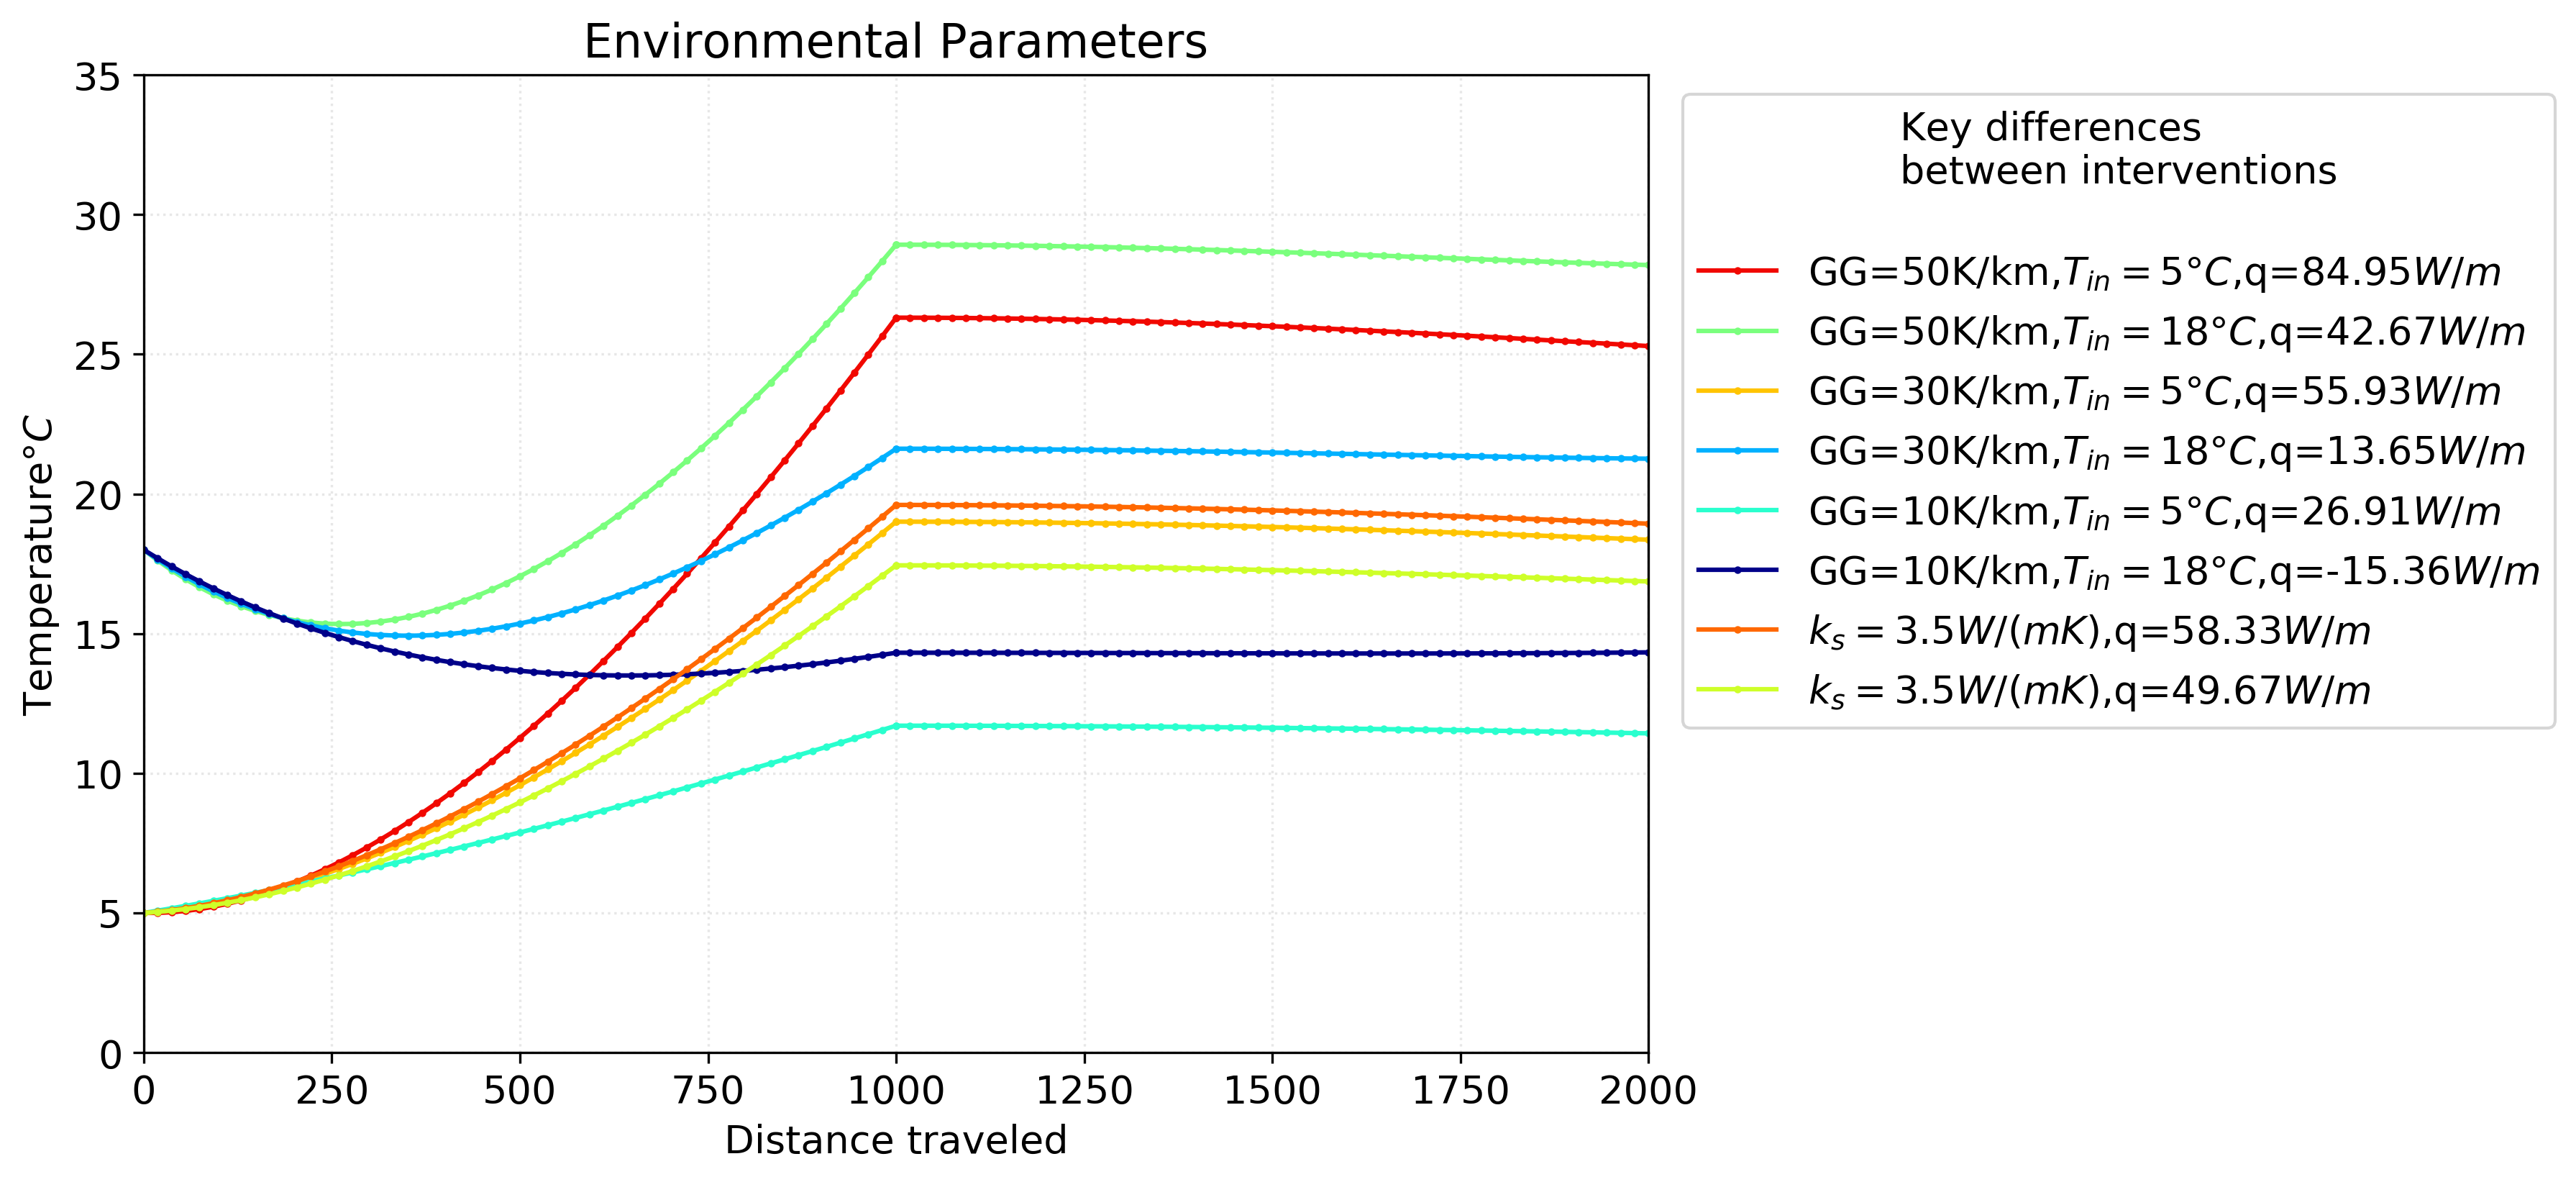
\includegraphics[width=0.75\textwidth]{EnvVars.png}
	            
	            \caption{Temperatuer variation along distance traveled for different CBHE configurations for design variables (top) and environmental parameters (bottom), $L=1000m$, $T_{in}=5\degree C$ and $w=0.058m^3/s$ as well as 30 Kelvin/km geothermal gradient before otherwise specified.}
	            \label{fig:TempCOP}
	        \end{figure}
	    As was pointed out in the discussion for varying the flow rate, however, an alternative to achieve maxmized COP with a minimized implication on geothermal depletion can also be achieved by using a significantly increased flow rate to achieve turbulence flow inside the inner pipe, so that the temperature increase at the bottom of the CBHE can be maintained at the outlet. The resulting COP from the CBHE will likely not only be a function of the temperature out, the flow rate, but also the amount of pumping power (operational cost) that went into ensuring the functioning of the overall system, which goes beyond the scope of this current paper. 
